%%%%%%%%%%%%%%%%%%%%%%%%%%%%%%%%%%%%%%%%%%%%%%%%%%
% SPECIALIZATION PROJECT REPORT
% Autonomous Video Ad-Placement and Contextual Safety Analyzer
% Department of Computer Science
% CHRIST (Deemed to be University)
%%%%%%%%%%%%%%%%%%%%%%%%%%%%%%%%%%%%%%%%%%%%%%%%%%

% CHANGED FROM THE SUPPLIED TEMPLATE: oneside, not "twoside, openright".
% The template forced every chapter onto a recto page, which inserted four
% blank pages into the front matter (they appeared as pages ii, iv, vi and
% viii, carrying nothing but a running header). oneside removes them and keeps
% the 1.5in binding margin on every page instead of alternating it, which is
% what a single-sided printed submission wants.
\documentclass[
12pt,
a4paper,
oneside
]{report}

%%%%%%%%%%%%%%%%%%%%%%%%%%%%%%%%%%%%%%%%%%%%%%%%%%
% PACKAGES
%%%%%%%%%%%%%%%%%%%%%%%%%%%%%%%%%%%%%%%%%%%%%%%%%%

\usepackage[
left=1.5in,
right=1in,
top=1in,
bottom=1in
]{geometry}

%%%%%%%%%%%%%%%%%%%%%%%%%%%%%%%%%%%%%%%%%%%%%%%%%%
% DRAFT SWITCH -- diagnostic, and a fast way to iterate
%
% Flip this to \draftmodetrue and every image becomes an empty box showing
% only its filename. The document then compiles in a couple of seconds.
%
% Use it to split a compile problem in two: if draft mode compiles and normal
% mode does not, the images are the cost and nothing else is wrong. Set it
% back to \draftmodefalse for the version you submit.
%%%%%%%%%%%%%%%%%%%%%%%%%%%%%%%%%%%%%%%%%%%%%%%%%%
\newif\ifdraftmode
\draftmodefalse

\usepackage{newtxtext,newtxmath}
\ifdraftmode
  \usepackage[draft]{graphicx}
\else
  \usepackage{graphicx}
\fi
\usepackage{setspace}
\usepackage{array}
\usepackage{longtable}
\usepackage{booktabs}
\usepackage{multirow}
\usepackage{float}
\usepackage{fancyhdr}
\usepackage{titlesec}
\usepackage{caption}
\usepackage{enumitem}
\usepackage[hidelinks]{hyperref}
\usepackage{url}
\usepackage{listings}
\usepackage{xcolor}

% REFERENCES: a plain thebibliography rather than biblatex + biber.
%
% biblatex runs biber as a separate program between LaTeX passes, which makes
% the build pdflatex -> biber -> pdflatex -> pdflatex. On a document this long
% that is a real cost, and Overleaf's free tier allows only about twenty
% seconds for the whole build. A static bibliography needs no external tool and
% one pass fewer, and with eighteen references it costs nothing to maintain.
%
% references.bib is kept in the project for reference and for anyone who wants
% to switch back; it is not read by this file.

%%%%%%%%%%%%%%%%%%%%%%%%%%%%%%%%%%%%%%%%%%%%%%%%%%
% SPACING
%%%%%%%%%%%%%%%%%%%%%%%%%%%%%%%%%%%%%%%%%%%%%%%%%%

\onehalfspacing

%%%%%%%%%%%%%%%%%%%%%%%%%%%%%%%%%%%%%%%%%%%%%%%%%%
% HEADER FOOTER
%%%%%%%%%%%%%%%%%%%%%%%%%%%%%%%%%%%%%%%%%%%%%%%%%%

\pagestyle{fancy}
\fancyhf{}
\fancyhead[L]{\small\textbf{BCA}}
\fancyhead[R]{\small\textbf{Specialization Project}}
\fancyfoot[C]{\thepage}
\renewcommand{\headrulewidth}{0.4pt}

%%%%%%%%%%%%%%%%%%%%%%%%%%%%%%%%%%%%%%%%%%%%%%%%%%
% CHAPTER STYLE
%%%%%%%%%%%%%%%%%%%%%%%%%%%%%%%%%%%%%%%%%%%%%%%%%%

\titleformat{\chapter}[display]
{\bfseries\Huge}
{\filcenter\chaptertitlename\ \thechapter}
{1ex}
{\filcenter}

%%%%%%%%%%%%%%%%%%%%%%%%%%%%%%%%%%%%%%%%%%%%%%%%%%
% CODE LISTING STYLE
%%%%%%%%%%%%%%%%%%%%%%%%%%%%%%%%%%%%%%%%%%%%%%%%%%

\definecolor{codegray}{rgb}{0.95,0.95,0.95}
\definecolor{codecomment}{rgb}{0.25,0.45,0.30}
\definecolor{codekey}{rgb}{0.00,0.19,0.38}

\lstset{
  backgroundcolor=\color{codegray},
  basicstyle=\ttfamily\scriptsize,
  keywordstyle=\color{codekey}\bfseries,
  commentstyle=\color{codecomment}\itshape,
  breaklines=true,
  captionpos=b,
  frame=single,
  showstringspaces=false,
  numbers=left,
  numberstyle=\tiny,
  xleftmargin=2em,
  framexleftmargin=1.5em
}

%%%%%%%%%%%%%%%%%%%%%%%%%%%%%%%%%%%%%%%%%%%%%%%%%%
% BEGIN DOCUMENT
%%%%%%%%%%%%%%%%%%%%%%%%%%%%%%%%%%%%%%%%%%%%%%%%%%

\begin{document}

\pagenumbering{roman}

%%%%%%%%%%%%%%%%%%%%%%%%%%%%%%%%%%%%%%%%%%%%%%%%%%
% COVER PAGE
%%%%%%%%%%%%%%%%%%%%%%%%%%%%%%%%%%%%%%%%%%%%%%%%%%

% Spacing reduced from the template's values. The template's placeholder title
% was one line; this one is four \Huge lines, and at the original spacing the
% page overflowed and the last two lines fell onto a second page. \singlespacing
% here as well -- \onehalfspacing applies to the title block otherwise and costs
% another two centimetres.
\begin{titlepage}
\begin{center}
\singlespacing

\vspace*{0.3cm}

{\Large\bfseries SPECIALIZATION PROJECT REPORT}

\vspace{0.7cm}

{\Huge\bfseries\begin{spacing}{1.12}%
\MakeUppercase{Autonomous Video Ad-Placement and Contextual Safety Analyzer}%
\end{spacing}}

\vspace{1.0cm}

A Project Report submitted in partial fulfillment of the requirements for the
award of the degree of

\vspace{0.4cm}

{\Large\bfseries BACHELOR OF COMPUTER APPLICATIONS}

\vspace{0.7cm}

by

\vspace{0.4cm}

\textbf{Andrew Shelton S}
Register No: 2441609\\[0.15cm]

\textbf{Akash Ganesh}
Register No: 2441604\\[0.15cm]

\textbf{Andrew Judah}
Register No: 2441608\\[0.15cm]

\textbf{Ramona Elisha Mary}
Register No: 2441646

\vspace{0.7cm}

Under the Guidance of

\vspace{0.25cm}

\textbf{Dr. Chanti}\\
Assistant Professor

\vspace{0.4cm}


\includegraphics[width=3.4cm]{Images/CU_logo_blue.png}

\vspace{0.4cm}

\textbf{DEPARTMENT OF COMPUTER SCIENCE}\\
School of Sciences\\
CHRIST (Deemed to be University)\\
Bengaluru, Karnataka, India

\vspace{0.4cm}

\textbf{AUGUST 2026}

\end{center}
\end{titlepage}

%%%%%%%%%%%%%%%%%%%%%%%%%%%%%%%%%%%%%%%%%%%%%%%%%%
% INNER TITLE PAGE
%%%%%%%%%%%%%%%%%%%%%%%%%%%%%%%%%%%%%%%%%%%%%%%%%%

\begin{titlepage}
\begin{center}
\singlespacing

\vspace*{1.0cm}

{\Huge\bfseries\begin{spacing}{1.12}%
\MakeUppercase{Autonomous Video Ad-Placement and Contextual Safety Analyzer}%
\end{spacing}}

\vspace{1.1cm}

A Specialization Project Report

\vspace{0.3cm}

Submitted in partial fulfillment of the requirements for the award of the
degree of

\vspace{0.4cm}

{\Large\bfseries BACHELOR OF COMPUTER APPLICATIONS}

\vspace{0.9cm}

by

\vspace{0.5cm}

\textbf{Andrew Shelton S}
Register No: 2441609

\textbf{Akash Ganesh}
Register No: 2441604

\textbf{Andrew Judah}
Register No: 2441608

\textbf{Ramona Elisha Mary}
Register No: 2441646

\vspace{1.2cm}

Under the Guidance of

\vspace{0.4cm}

\textbf{Dr. Chanti}\\
Assistant Professor

\vfill


\includegraphics[width=4cm]{Images/CU_logo_blue.png}

\vspace{0.5cm}

{\large\bfseries DEPARTMENT OF COMPUTER SCIENCE}\\
School of Sciences\\
CHRIST (Deemed to be University)\\
Bengaluru, Karnataka, India

\vspace{0.5cm}

{\bfseries AUGUST 2026}

\end{center}
\end{titlepage}

%%%%%%%%%%%%%%%%%%%%%%%%%%%%%%%%%%%%%%%%%%%%%%%%%%
% CERTIFICATE
%%%%%%%%%%%%%%%%%%%%%%%%%%%%%%%%%%%%%%%%%%%%%%%%%%

\chapter*{Certificate}
\addcontentsline{toc}{chapter}{Certificate}

This is to certify that the project report entitled ``\textbf{Autonomous Video
Ad-Placement and Contextual Safety Analyzer}'' is a bona fide record of the work
carried out by Andrew Shelton S (2441609), Akash Ganesh (2441604), Andrew Judah
(2441608) and Ramona Elisha Mary (2441646) of CHRIST (Deemed to be University),
Bangalore, in partial fulfilment of the academic requirements for the degree of
Bachelor of Computer Applications during the academic year 2026--27.

The work documented in this report includes the analysis, design, development,
implementation, testing and evaluation of the proposed Autonomous Video
Ad-Placement and Contextual Safety Analyzer. The project demonstrates the
application of the knowledge and skills acquired during the programme to address
the identified problem and develop an appropriate technological solution.

The project work has been carried out under the guidance and supervision of
Dr. Chanti, Assistant Professor, Department of Computer Science, and is
submitted in partial fulfilment of the academic requirements of the programme.

\vspace{0.6cm}

\noindent\textbf{Student Details}

\begin{enumerate}[itemsep=2pt]
\item Andrew Shelton S (2441609)
\item Akash Ganesh (2441604)
\item Andrew Judah (2441608)
\item Ramona Elisha Mary (2441646)
\end{enumerate}

\vspace{2.5cm}

\noindent
Guide Signature
\hfill
Head of Department

\vspace{1.5cm}
\noindent
Valued By: (Name and Signature)\\

%%%%%%%%%%%%%%%%%%%%%%%%%%%%%%%%%%%%%%%%%%%%%%%%%%
% DECLARATION
%%%%%%%%%%%%%%%%%%%%%%%%%%%%%%%%%%%%%%%%%%%%%%%%%%

\chapter*{Declaration}
\addcontentsline{toc}{chapter}{Declaration}

We hereby declare that the project entitled \textbf{``Autonomous Video
Ad-Placement and Contextual Safety Analyzer''} is our original academic work
carried out as part of the requirements for the degree of \textbf{Bachelor of
Computer Applications} at \textbf{CHRIST (Deemed to be University), Bangalore}.

We further declare that the work presented in this report has been undertaken by
us and that the report accurately represents the \textbf{implementation,
analysis, testing, and evaluation} carried out as part of the project.

The report clearly distinguishes between \textbf{implemented functionality,
dataset-backed analysis, modeled functionality, and proposed future work},
wherever applicable. In particular, Section~\ref{sec:accuracy} states plainly
that no accuracy figure is claimed on real creator footage, because the
labelled evidence required to support one has not been assembled.

We accept responsibility for the accuracy of the implementation details,
interpretation of project results, and academic integrity of this report.

\vspace{0.7cm}

\begin{flushleft}
\textbf{Andrew Shelton S}\\
Register No.: 2441609\\
Signature: \hspace{3cm} Date: \\[.5cm]

\textbf{Akash Ganesh}\\
Register No.: 2441604\\
Signature: \hspace{3cm} Date: \\[.5cm]

\textbf{Andrew Judah}\\
Register No.: 2441608\\
Signature: \hspace{3cm} Date: \\[.5cm]

\textbf{Ramona Elisha Mary}\\
Register No.: 2441646\\
Signature: \hspace{3cm} Date:
\end{flushleft}

%%%%%%%%%%%%%%%%%%%%%%%%%%%%%%%%%%%%%%%%%%%%%%%%%%
% ACKNOWLEDGEMENT
%%%%%%%%%%%%%%%%%%%%%%%%%%%%%%%%%%%%%%%%%%%%%%%%%%

\chapter*{Acknowledgement}
\addcontentsline{toc}{chapter}{Acknowledgement}

We express our sincere thanks to all faculty members and staff of the
\textbf{Department of Computer Science, CHRIST (Deemed to be University),
Bangalore}, for their valuable suggestions, support, and encouragement
throughout the course of this project.

First of all, we thank \textbf{God Almighty} for His immense grace and blessings
showered upon us at every stage of this work.

We are grateful to our respected \textbf{Head of the Department, Department of
Computer Science, CHRIST (Deemed to be University)}, for providing us with the
opportunity to undertake this project as part of our curriculum. We also express
our sincere gratitude to the \textbf{Associate Head of the Department,
Department of Computer Science}, for the continuous support and encouragement
provided throughout the project.

We would also like to express our gratitude to the \textbf{Coordinator,
Department of Computer Science, CHRIST (Deemed to be University)}, for the
valuable guidance and support extended during the various stages of the project.

We are deeply grateful to our \textbf{Project In-charge and Guide, Dr. Chanti,
Assistant Professor, Department of Computer Science}, for the continuous
guidance, valuable suggestions, constructive feedback, and encouragement
provided throughout the project. The guidance and support received during every
stage of the project greatly contributed to its successful completion.

We would also like to thank our \textbf{Alumni Evaluator} for the valuable
feedback, suggestions, and industry-oriented insights that helped us improve the
project and make the necessary changes in accordance with professional and
industry standards.

Finally, we would like to express our sincere gratitude to everyone who
contributed to this project, directly or indirectly, and supported us in
successfully completing this work.

\vspace{0.5cm}
\noindent
Name of the Student(s): Andrew Shelton S, Akash Ganesh, Andrew Judah,
Ramona Elisha Mary \\
Reg No.: 2441609, 2441604, 2441608, 2441646 \\
Date:

%%%%%%%%%%%%%%%%%%%%%%%%%%%%%%%%%%%%%%%%%%%%%%%%%%
% ABSTRACT
%%%%%%%%%%%%%%%%%%%%%%%%%%%%%%%%%%%%%%%%%%%%%%%%%%

\chapter*{Abstract}
\addcontentsline{toc}{chapter}{Abstract}

Video platforms decide whether a video may carry advertising by classifying it
automatically, at scale, after publication. The creator learns the outcome only
once the video is live and its first hours of traffic --- the most valuable
hours --- have already passed. The verdict arrives as a label with no reasoning
attached, and appeals are slow. There is no equivalent of a compiler warning: no
way to ask, before publishing, what in a video is likely to cause trouble and
where in the runtime it occurs.

This project builds that missing pre-publication check. \textbf{AdSafe Studio} is
an offline desktop application that audits a video file on the creator's own
machine and reports, against a timeline, every finding that bears on
advertiser suitability, together with the surfaces in the frame where an
advertisement could reasonably be placed.

The system has four analysis engines that run in sequence. An audio and language
engine extracts the audio track, transcribes it with faster-whisper at
word-level granularity, and matches each word against a configurable restricted
vocabulary. A vision engine samples frames and runs object detection at two
resolutions, merging the results, using a YOLOv8 model fine-tuned by the team on
an Open Images V7 subset because no freely available pretrained model covers the
required risk classes. An advertisement-placement engine locates the largest
unoccupied rectangle in each frame and keeps only those surfaces that persist
for five seconds or more. An overlay-context engine measures per-pixel temporal
variance to detect persistent on-screen graphics, which allows a weapon rendered
inside a game to be weighed differently from one filmed in reality. A
three-state verdict --- Monetizable, Review or Restricted --- is then computed,
and the reasoning that produced it is printed alongside it.

The implementation comprises approximately 6{,}100 lines of Python and
JavaScript across a FastAPI backend, a SQLite data layer and a React interface
of seven screens, covered by 175 automated tests. Analysis is performed entirely
on local hardware; the application makes no external network request of any
kind, a property verified by an automated check that severs all non-local
traffic and confirms the interface still renders correctly.

Evaluation was conducted on real video rather than on validation metrics alone,
and that decision proved decisive: a second fine-tuning run that improved every
headline validation metric was rejected after it detected a real firearm zero
times where the accepted model detected it thirteen times. Four separate real
clips each exposed a defect that synthetic testing had not. No precision figure
is claimed on creator footage, because the labelled benchmark corpus required to
support such a claim has not been assembled; the benchmark harness is built and
refuses, by design, to publish a figure from insufficient evidence.

Future work centres on completing that labelled corpus, extending the risk
taxonomy to classes that the current dataset cannot supply, and suppressing
advertisement surfaces that fall inside detected overlay regions.

\vspace{0.4cm}
\noindent\textbf{Keywords:} brand safety, object detection, speech recognition,
advertisement placement, offline processing, YOLOv8, faster-whisper.

\newpage
\tableofcontents

\newpage
\listoffigures

\newpage
\listoftables

\newpage

\chapter*{List of Abbreviations}
\addcontentsline{toc}{chapter}{List of Abbreviations}

\begin{longtable}{p{4cm}p{9cm}}
AGPL & Affero General Public License \\
AI & Artificial Intelligence \\
API & Application Programming Interface \\
COCO & Common Objects in Context (dataset) \\
COCOMO & Constructive Cost Model \\
CSV & Comma-Separated Values \\
DBMS & Database Management System \\
DFD & Data Flow Diagram \\
ERD & Entity Relationship Diagram \\
FPS & Frames Per Second \\
GPU & Graphics Processing Unit \\
HUD & Heads-Up Display \\
IoU & Intersection over Union \\
JSON & JavaScript Object Notation \\
KLOC & Thousand Lines of Code \\
mAP & Mean Average Precision \\
ML & Machine Learning \\
ORM & Object Relational Mapping \\
REST & Representational State Transfer \\
SPA & Single Page Application \\
SQL & Structured Query Language \\
SRS & Software Requirements Specification \\
UI & User Interface \\
UML & Unified Modeling Language \\
WAL & Write-Ahead Logging \\
YOLO & You Only Look Once (detection architecture) \\
\end{longtable}

\newpage

\pagenumbering{arabic}

%%%%%%%%%%%%%%%%%%%%%%%%%%%%%%%%%%%%%%%%%%%%%%%%%%
\chapter{Introduction}
%%%%%%%%%%%%%%%%%%%%%%%%%%%%%%%%%%%%%%%%%%%%%%%%%%

\section{Introduction}

A video creator who depends on advertising revenue works without a compiler.
Software is checked before it ships; a video is checked after it publishes. The
platform's classifier examines the file once it is live, applies a label, and
the creator discovers the outcome from a dashboard --- typically after the first
hours of traffic, which carry the highest revenue per view, are already gone.

The label arrives without reasoning. A video is marked as unsuitable for most
advertisers, but not which second of it, not which word, not which object. The
creator is left to guess, re-edit and re-upload, or to appeal through a process
measured in days.

This project addresses that gap directly. It builds a tool that performs the
check \emph{before} publication, on the creator's own machine, and reports its
findings against the video's timeline so that each one can be located, watched
and judged. Where the platform gives a verdict, this system gives a verdict
\emph{and} the evidence for it.

A second and less obvious opportunity sits alongside the first. The same frame
analysis that locates a risk can also locate its opposite: regions of the frame
that stay visually empty for long enough to carry an overlay advertisement
without obscuring the content. Detecting risk and detecting inventory are the
same scan performed with opposite intent.

\section{Objectives}

\begin{enumerate}[itemsep=3pt]
\item To ingest a video file, extract its technical metadata, and store both the
file and its metadata in a local database.
\item To transcribe the spoken audio of a video with word-level timestamps and
identify occurrences of a configurable restricted vocabulary.
\item To detect visually sensitive objects in sampled frames using an object
detection model trained for the project's risk taxonomy.
\item To identify continuous regions of the frame that remain unoccupied for a
sustained period and are therefore suitable for advertisement placement.
\item To distinguish rendered on-screen content, such as game overlays, from
filmed content, so that a rendered object is not treated as a real hazard.
\item To produce a three-state advertiser-suitability verdict accompanied by the
explicit reasoning that produced it.
\item To present all findings on a navigable timeline and export them as PDF,
CSV and JSON audit reports.
\item To perform the entire analysis on local hardware, with no dependence on
any external service.
\end{enumerate}

\section{Identification of Need}

The need arises from three properties of the current arrangement.

\textbf{The decision is post-hoc.} Classification happens after publication.
Whatever revenue is lost during the review-and-appeal window is not recoverable,
and that window overlaps precisely with the period in which a video earns most
of its lifetime revenue.

\textbf{The decision is unexplained.} Platform guidelines describe categories of
unsuitable content \cite{YouTubeAdFriendly} but the classifier does not report
which part of a given video triggered which category. A creator cannot fix what
is not localised.

\textbf{The decision cannot distinguish depiction from context.} A firearm on
screen is a firearm to a detector, whether it is held by a person in a
documentary or rendered by a game engine in a first-person shooter. Gaming is
among the largest content categories on video platforms, so a system that cannot
make this distinction is of limited use to a very large group of creators. This
observation drives one of the project's more distinctive components, described
in Section~\ref{sec:overlay}.

There is a further need specific to the creator's position: \textbf{privacy}.
Unpublished video is commercially sensitive. A tool that requires uploading
draft footage to a third-party service to check it is unattractive, and for
footage under embargo it is unusable. Local processing is not merely a technical
preference here; it is a precondition for the tool being adopted at all.

\section{Scope of the Project}

\textbf{Within scope.} Local ingestion of MP4, MOV and AVI files; speech
transcription and restricted-vocabulary matching with per-word timestamps;
object detection across a defined risk taxonomy; free-space advertisement
surface detection with a persistence threshold; persistent-overlay detection;
three-state verdict determination with printed reasoning; a seven-screen web
interface served locally; and export of audit reports in PDF, CSV and JSON.

\textbf{Outside scope.} The system does not upload to, or integrate with, any
video platform. It does not replicate any platform's proprietary classifier and
makes no claim to predict a specific platform's decision. It does not support
multiple user accounts, and it performs no authentication --- the reasoning for
that decision, and its consequences, are set out in Chapter~\ref{ch:security}.
It does not detect smoking or narcotics visually, because the source dataset
used for training does not supply usable classes for them; these are covered in
the audio vocabulary instead. It does not edit or re-encode video.

\section{Organization of the Report}

Chapter~2 examines how advertiser-suitability decisions are currently made and
establishes the feasibility of the proposed alternative. Chapter~3 documents the
project plan, schedule and risks. Chapter~4 identifies the software process
model and justifies it. Chapter~5 presents the system models. Chapter~6
describes the architecture, database and interface design. Chapter~7 documents
the implementation. Chapter~8 reports testing, including the results that
changed the design. Chapter~\ref{ch:security} sets out the security posture.
Chapter~10 estimates cost. Chapter~11 presents the system's reports and output
screens. Chapter~12 concludes and identifies future work. The appendices carry
source extracts, the user manual, database scripts and supporting material.

%%%%%%%%%%%%%%%%%%%%%%%%%%%%%%%%%%%%%%%%%%%%%%%%%%
\chapter{System Analysis}
%%%%%%%%%%%%%%%%%%%%%%%%%%%%%%%%%%%%%%%%%%%%%%%%%%

\section{Preliminary Investigation}

The investigation began by establishing how advertiser-suitability decisions are
actually made today, and what tooling a creator can obtain to anticipate them.

Platforms publish guidelines describing categories of content that limit or
remove advertising: violence, adult themes, controversial issues, harmful
substances, inappropriate language and similar \cite{YouTubeAdFriendly}. The
classification itself is automated and applied to essentially all uploads.
Manual review exists but functions as an appeal path rather than a first pass.

The investigation then examined what a creator can do in advance. The available
options fall into three groups: reading the guidelines and self-assessing;
uploading privately and reading the resulting label before going public; or
using third-party services that estimate brand-safety risk. Each is examined
below.

Finally, the investigation examined whether the technical components required
for a local tool were available. Speech recognition of sufficient quality can
now run on a laptop CPU \cite{Radford2023, CTranslate2}. General-purpose object
detection is mature and fast \cite{Redmon2016, Jocher2023}. The gap --- and this
proved to be the project's central technical problem --- is that no widely
available pretrained detector covers the specific risk classes required. This is
examined in Section~\ref{sec:taxonomy}.

\section{Existing System}

Three approaches are in current use.

\textbf{Platform-side automated classification.} The platform inspects the video
after upload and assigns a monetisation state. It is comprehensive and free, and
it is the decision that actually matters commercially. It is also opaque, late,
and offers no localisation of the cause.

\textbf{Manual self-review against published guidelines.} The creator reads the
guidelines and judges their own footage. This is available before publication
and costs nothing, but it does not scale to long-form content, it is
inconsistent between people, and it depends on the creator remembering every
moment of a multi-hour recording.

\textbf{Third-party brand-safety services.} Commercial services analyse video
and report risk scores. These are designed for advertisers and agencies
assessing inventory at scale rather than for individual creators checking a
draft. They are priced accordingly, and they require the footage to be uploaded
to the vendor.

\section{Limitations of Existing System}

\begin{enumerate}[itemsep=3pt]
\item \textbf{The verdict arrives after publication.} The revenue lost in the
review window is not recoverable.
\item \textbf{The verdict is not explained.} No timestamp, word or object is
identified, so the creator cannot act on it precisely.
\item \textbf{Rendered content is not distinguished from filmed content.} A
weapon in gameplay footage and a weapon in a news report are the same signal to
a detector operating on frames alone.
\item \textbf{Draft footage must leave the creator's machine.} Both the
upload-privately approach and third-party services require transferring
unpublished material to a third party.
\item \textbf{Nothing identifies advertisement inventory.} Existing tools assess
risk only. None report where in the frame an overlay could be placed without
obscuring the content.
\end{enumerate}

\section{Proposed System}

The proposed system is a locally installed application that a creator runs
against a video file before publishing it. It produces four categories of
output.

\textbf{Audio findings.} Each occurrence of a restricted term, with its
timestamp, the surrounding transcript for context, an assigned severity, and the
name of the engine that produced it.

\textbf{Visual findings.} Each detected object of interest, with its frame
timestamp, bounding box, confidence, risk category, and again the producing
engine. Findings are reported by grouped term --- ``Handheld weapon'' rather
than ``Handgun'' --- with the model's own class retained alongside, because the
category is reliable in a way the specific class is not.

\textbf{Advertisement surfaces.} Each region of the frame that remains
unoccupied for at least five seconds, with its bounding box, area and a
suitability score.

\textbf{A verdict with reasoning.} One of Monetizable, Review or Restricted,
accompanied by the sentences that justify it, including any overlay evidence
that moderated the outcome.

Every one of these is computed on the local machine. No data leaves it. This is
verified rather than asserted: an automated check severs all non-local network
traffic and confirms the interface still functions, described in
Section~\ref{sec:offlinecheck}.

\section{Feasibility Study}

\subsection{Technical Feasibility}

The technical question was never whether the components existed, but whether
they could be made to work on the required content at acceptable speed on
ordinary hardware.

Speech recognition is feasible. faster-whisper, a CTranslate2 reimplementation
of Whisper, runs the \texttt{base.en} model on a laptop CPU at usable speed and
supplies word-level timestamps natively, which the data model requires
\cite{CTranslate2, Radford2023}.

Object detection is feasible but required work. Stock YOLOv8 is trained on the
COCO classes \cite{Lin2014, Jocher2023}, which contain no firearm, no cigarette
and no narcotic; only adjacent classes such as \texttt{knife} and
\texttt{bottle}. The project therefore trained its own model on an Open Images
V7 subset \cite{Kuznetsova2020}. This is documented in
Section~\ref{sec:taxonomy} and Chapter~8.

Advertisement-surface detection is feasible with a classical algorithm rather
than a learned one. Locating the largest empty rectangle is a maximal-rectangle
problem over a binary occupancy matrix, and is solved deterministically and
quickly.

\subsection{Economic Feasibility}

Direct cost is zero. Every component is open-source and every computation runs
on hardware the team already owns. The licensing position is stated explicitly
in Section~\ref{sec:licensing}, since Ultralytics YOLOv8 is AGPL-3.0 and that
licence extends to trained weights.

\subsection{Operational Feasibility}

The system is operated through a browser interface that deliberately follows the
conventions of existing video-management tools, so that the interaction model is
already familiar \cite{Nielsen2012}. A creator uploads a video, starts the
analysis and reads the findings on a timeline. No knowledge of machine learning
is required at any point.

\subsection{Schedule Feasibility}

The project was completed within the academic semester using an incremental
process in which each milestone replaced one stand-in component with a working
implementation while the remainder of the pipeline continued to operate. There
was therefore no phase during which the system did not run, and no integration
phase at the end.

\section{Chapter Summary}

This chapter examined how advertiser-suitability decisions are currently made
and identified their common weakness: a verdict issued without context and
without explanation, after publication rather than before. The proposed system
addresses this by auditing video locally before release, distinguishing rendered
content from filmed content, and reporting the reasoning behind every verdict.
The feasibility study confirms the approach is technically achievable,
economically practical and deliverable within the project timeline.

%%%%%%%%%%%%%%%%%%%%%%%%%%%%%%%%%%%%%%%%%%%%%%%%%%
\chapter{Project Planning}
%%%%%%%%%%%%%%%%%%%%%%%%%%%%%%%%%%%%%%%%%%%%%%%%%%

% NOTE: the supplied template contained this chapter twice, verbatim. Only one
% copy is retained here.

\section{Introduction}

Project planning identifies the tasks to be performed, allocates responsibility,
estimates duration and provides a basis for monitoring progress
\cite{Sommerville2016}. For this project, planning was organised around a
sequence of milestones, each replacing one stand-in component with a working
implementation. Because the pipeline remained operable throughout, each
milestone was independently demonstrable.

\section{Work Breakdown Structure}

The project was divided into four phases containing twelve work packages.

\begin{figure}[H]
\centering
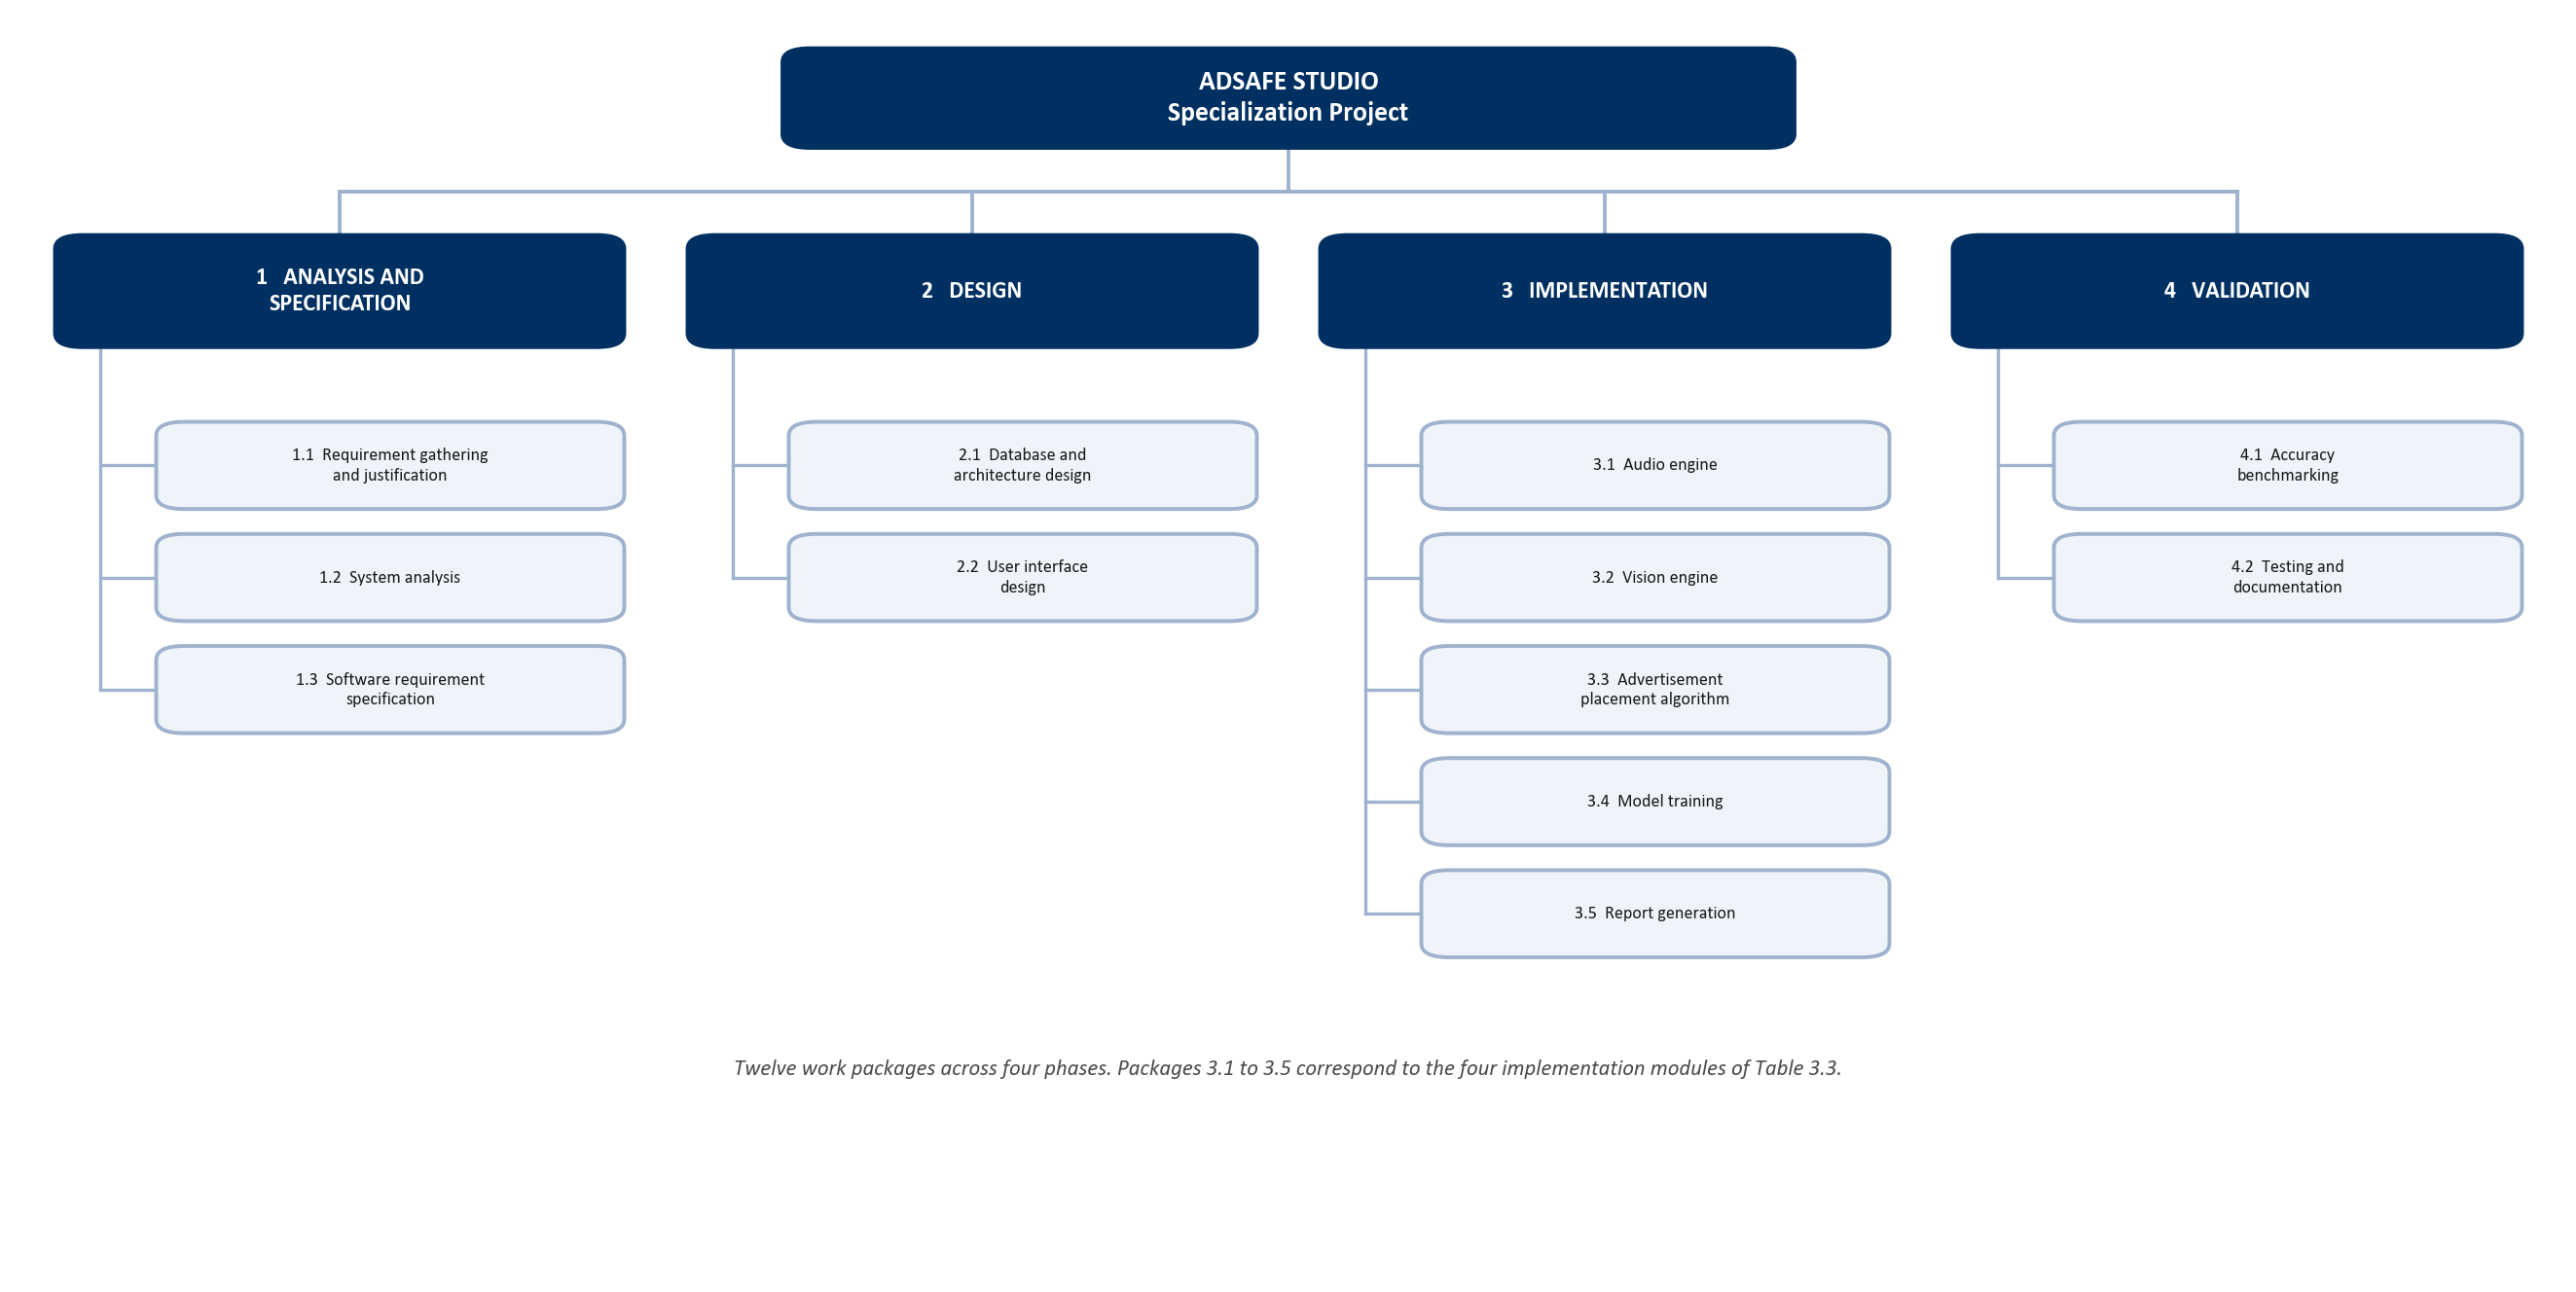
\includegraphics[width=0.95\textwidth]{Images/wbs.png}
\caption{Work Breakdown Structure}
\end{figure}

\section{Resource Planning}

The project is divided into four modules, each owned by one team member.

\begin{table}[H]
\centering
\begin{tabular}{|c|p{4.6cm}|p{5.4cm}|}
\hline
\textbf{Module} & \textbf{Scope} & \textbf{Implementation} \\
\hline
1 & Audio and natural language engine & Audio extraction, transcription,
keyword matching, severity assignment \\
\hline
2 & Vision and advertisement placement & Frame sampling, object detection,
model fine-tuning, free-space algorithm, overlay detection \\
\hline
3 & Orchestration, database and API & Pipeline sequencing, data layer,
migrations, REST endpoints, reporting \\
\hline
4 & Web user interface & React application, seven screens, timeline, reporting
views, responsive layout \\
\hline
\end{tabular}
\caption{Module Allocation}
\end{table}

Beyond people, the project required a laptop-class development machine per team
member, approximately 5\,GB of local storage for model weights and analysis
data, and one session of donated GPU time on Google Colab for the second
fine-tuning run.

\section{Risk Analysis}

\begin{table}[H]
\centering
\begin{tabular}{|p{4.8cm}|c|p{5.6cm}|}
\hline
\textbf{Risk} & \textbf{Severity} & \textbf{Mitigation} \\
\hline
No pretrained model covers the required risk classes & High & Train a model
specifically for the project on an openly licensed dataset \\
\hline
Validation accuracy does not predict behaviour on real video & High & Evaluate
every candidate model on real footage before accepting it \\
\hline
Accuracy claim unsupported by measurement & High & Build a benchmark harness
that refuses to publish a figure from insufficient evidence \\
\hline
Detection of rendered objects treated as real hazards & Medium & Detect
persistent overlays and weigh them against visual findings \\
\hline
Model inference too slow on laptop hardware & Medium & Sample frames rather
than process every frame; cap analysis resolution \\
\hline
Demonstration output mistaken for measured output & Medium & Record the
producing engine against every finding and display it \\
\hline
\end{tabular}
\caption{Risk Analysis}
\end{table}

The first two risks materialised, and both mitigations were exercised. They are
reported in Chapter~8.

\section{Project Scheduling}

The project activities are scheduled across a period of 14 weeks.

\begin{table}[H]
\centering
\begin{tabular}{|c|p{8cm}|c|}
\hline
\textbf{Task ID} & \textbf{Activity} & \textbf{Duration (Weeks)}\\
\hline
T1 & Requirement Gathering and Justification & 1\\
\hline
T2 & System Analysis & 1\\
\hline
T3 & SRS Preparation & 1\\
\hline
T4 & Database and Architecture Design & 1\\
\hline
T5 & User Interface Design and Implementation & 2\\
\hline
T6 & Audio Engine Implementation & 1\\
\hline
T7 & Vision Engine Implementation & 2\\
\hline
T8 & Advertisement Placement Algorithm & 1\\
\hline
T9 & Model Training and Evaluation & 1\\
\hline
T10 & Report Generation & 1\\
\hline
T11 & Accuracy Benchmarking & 1\\
\hline
T12 & Testing and Documentation & 1\\
\hline
\end{tabular}
\caption{Project Schedule}
\end{table}

\section{PERT Chart}

The database and architecture design must be complete before any engine can
store its findings, so tasks T6 through T8 all depend on T4. The audio and
vision engines are independent of one another. Benchmarking depends on every
engine being complete, which places T11 on the critical path.

\begin{figure}[H]
\centering
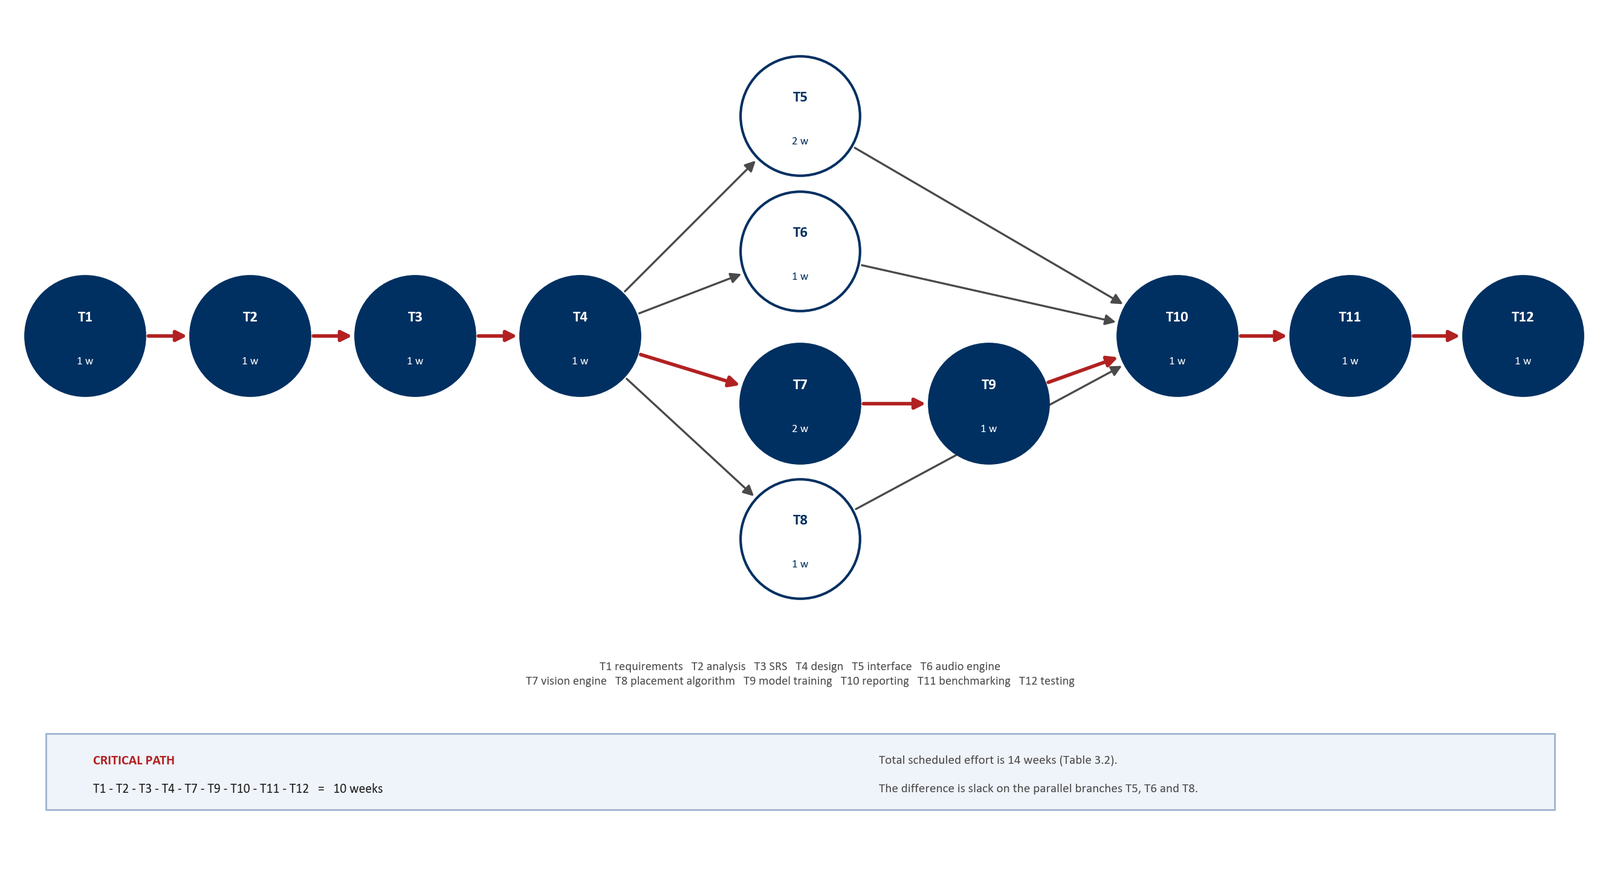
\includegraphics[width=0.95\textwidth]{Images/pert.png}
\caption{PERT Chart}
\end{figure}

The critical path is T1--T2--T3--T4--T7--T9--T10--T11--T12, a length of ten
weeks. The schedule in Table~3.2 allocates fourteen weeks in total; the
difference is slack carried on the parallel branches T5, T6 and T8.

\section{Gantt Chart}

\begin{figure}[H]
\centering
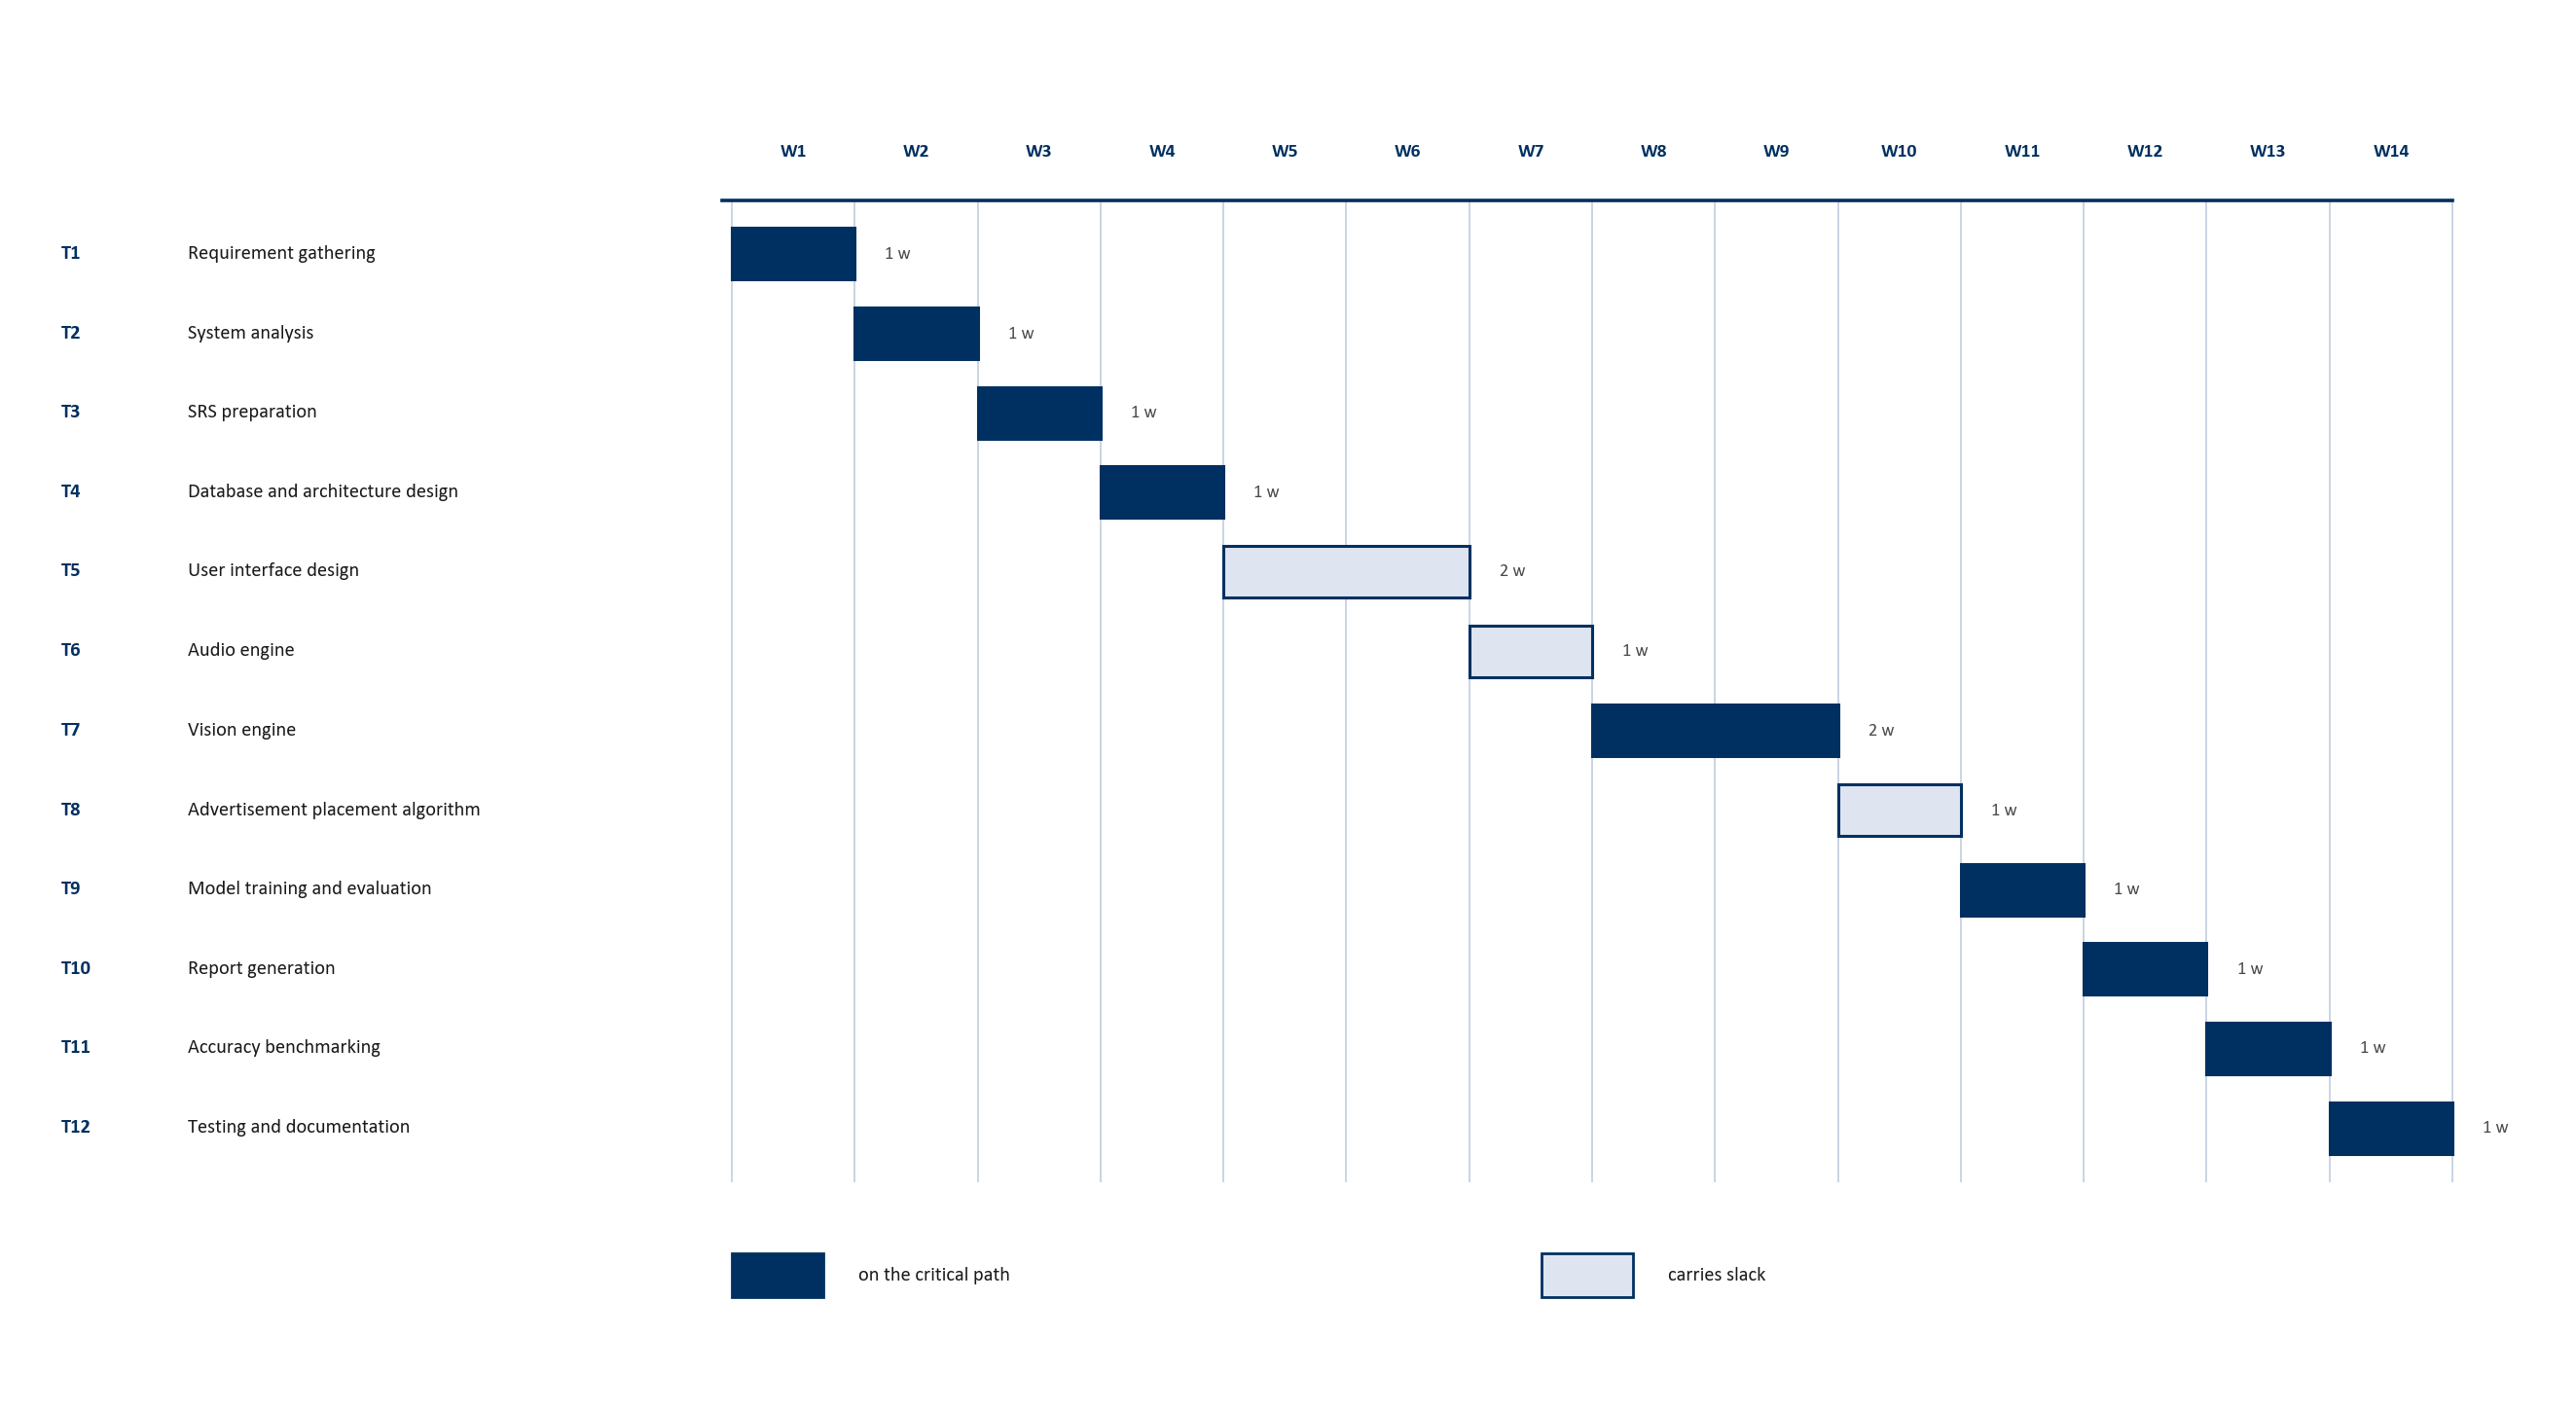
\includegraphics[width=0.95\textwidth]{Images/gantt.png}
\caption{Gantt Chart}
\end{figure}

%%%%%%%%%%%%%%%%%%%%%%%%%%%%%%%%%%%%%%%%%%%%%%%%%%
\chapter{Software Engineering Paradigm}
%%%%%%%%%%%%%%%%%%%%%%%%%%%%%%%%%%%%%%%%%%%%%%%%%%

\section{Introduction}

The choice of a software process model determines how requirements, design,
implementation and testing are sequenced \cite{Pressman2015}. This chapter
identifies the model adopted and the reasoning behind that selection.

\section{Selected Development Model}

The project follows the \textbf{Incremental Model}. A core skeleton is built
first, and each subsequent increment adds one working capability to a system
that already runs. The phases within each increment are requirement analysis,
design, implementation, testing and integration, and evaluation before
proceeding.

\begin{figure}[H]
\centering
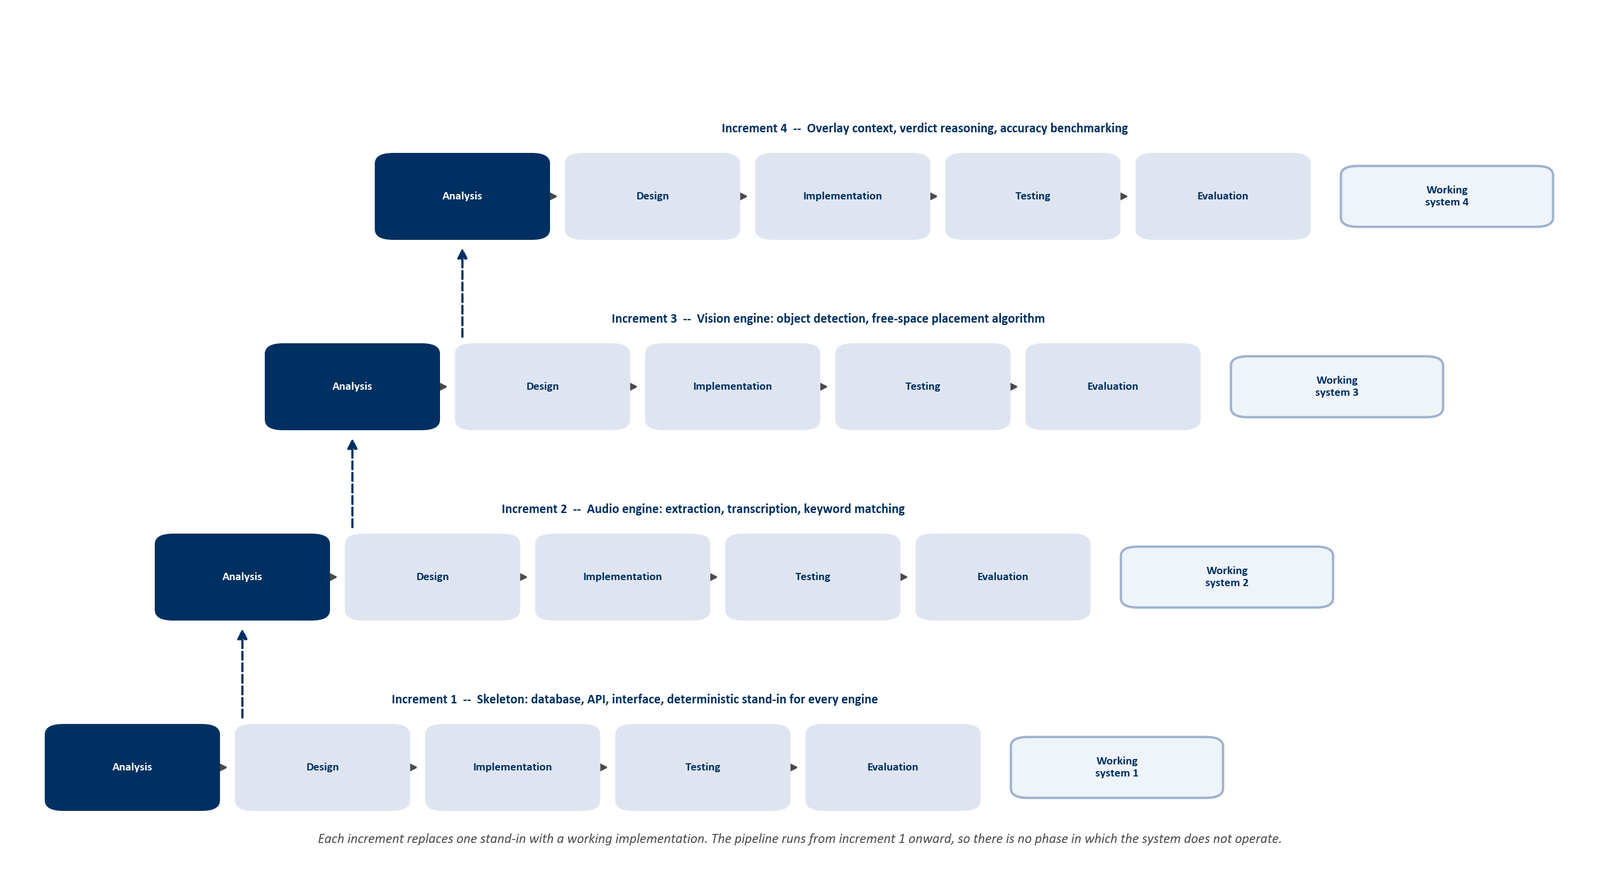
\includegraphics[width=0.95\textwidth]{Images/incremental.png}
\caption{Incremental Development Model}
\end{figure}

\section{Justification}

\begin{itemize}[itemsep=4pt]
\item \textbf{The system had to remain demonstrable throughout.} Deterministic
stand-in components were written for each engine at the outset, so the full
pipeline operated from the first week. Each increment replaced one stand-in
without interrupting the rest.

\item \textbf{Component feasibility could not be established in advance.}
Whether a freely available model could detect the required risk classes was
unknown until it was tested. A model requiring the design to be fixed before
implementation begins cannot accommodate that.

\item \textbf{Measurement changed the design.} Several decisions were reversed
on evidence produced during implementation, including the choice to train a
model rather than adopt an existing one, and the rejection of a fine-tuning run
that scored better on every validation metric. An incremental process allows a
decision to be revisited when measurement contradicts it.

\item \textbf{The academic timeline is fixed.} If an increment overruns, the
system remains functional without it, and the increment can be reduced in scope
rather than jeopardising delivery.
\end{itemize}

\section{Development Methodology}

Work proceeded in four increments.

\begin{table}[H]
\centering
\begin{tabular}{|c|p{4.2cm}|p{6cm}|}
\hline
\textbf{Increment} & \textbf{Capability added} & \textbf{Outcome} \\
\hline
1 & Skeleton: database, API, interface, deterministic stand-ins & A running
end-to-end pipeline in week one, usable for demonstration \\
\hline
2 & Audio engine & Real transcription and vocabulary matching with word-level
timestamps \\
\hline
3 & Vision engine and placement & Real object detection, a fine-tuned risk
model, and free-space surface detection \\
\hline
4 & Overlay context, verdict reasoning, benchmarking & Rendered content
distinguished from filmed; three-state verdict with printed reasoning \\
\hline
\end{tabular}
\caption{Development Methodology}
\end{table}

Version control was used throughout, with each change recorded as a separate
commit carrying a message that states what changed and why. The repository
history therefore functions as the project's engineering record and is cited in
several places in this report.

%%%%%%%%%%%%%%%%%%%%%%%%%%%%%%%%%%%%%%%%%%%%%%%%%%
\chapter{System Modeling}
%%%%%%%%%%%%%%%%%%%%%%%%%%%%%%%%%%%%%%%%%%%%%%%%%%

\section{Introduction}

This chapter presents the models describing the structure and behaviour of the
system: data flow, use cases, activity, sequence, state, class structure, the
entity relationship model and control flow.

\section{Data Flow Diagram Level 0}

The Level 0 diagram provides a context view. The system interacts with two
external entities: the Creator, who supplies video and receives audit findings;
and the Local Model Store, which supplies the transcription and detection
weights.

\begin{figure}[H]
\centering
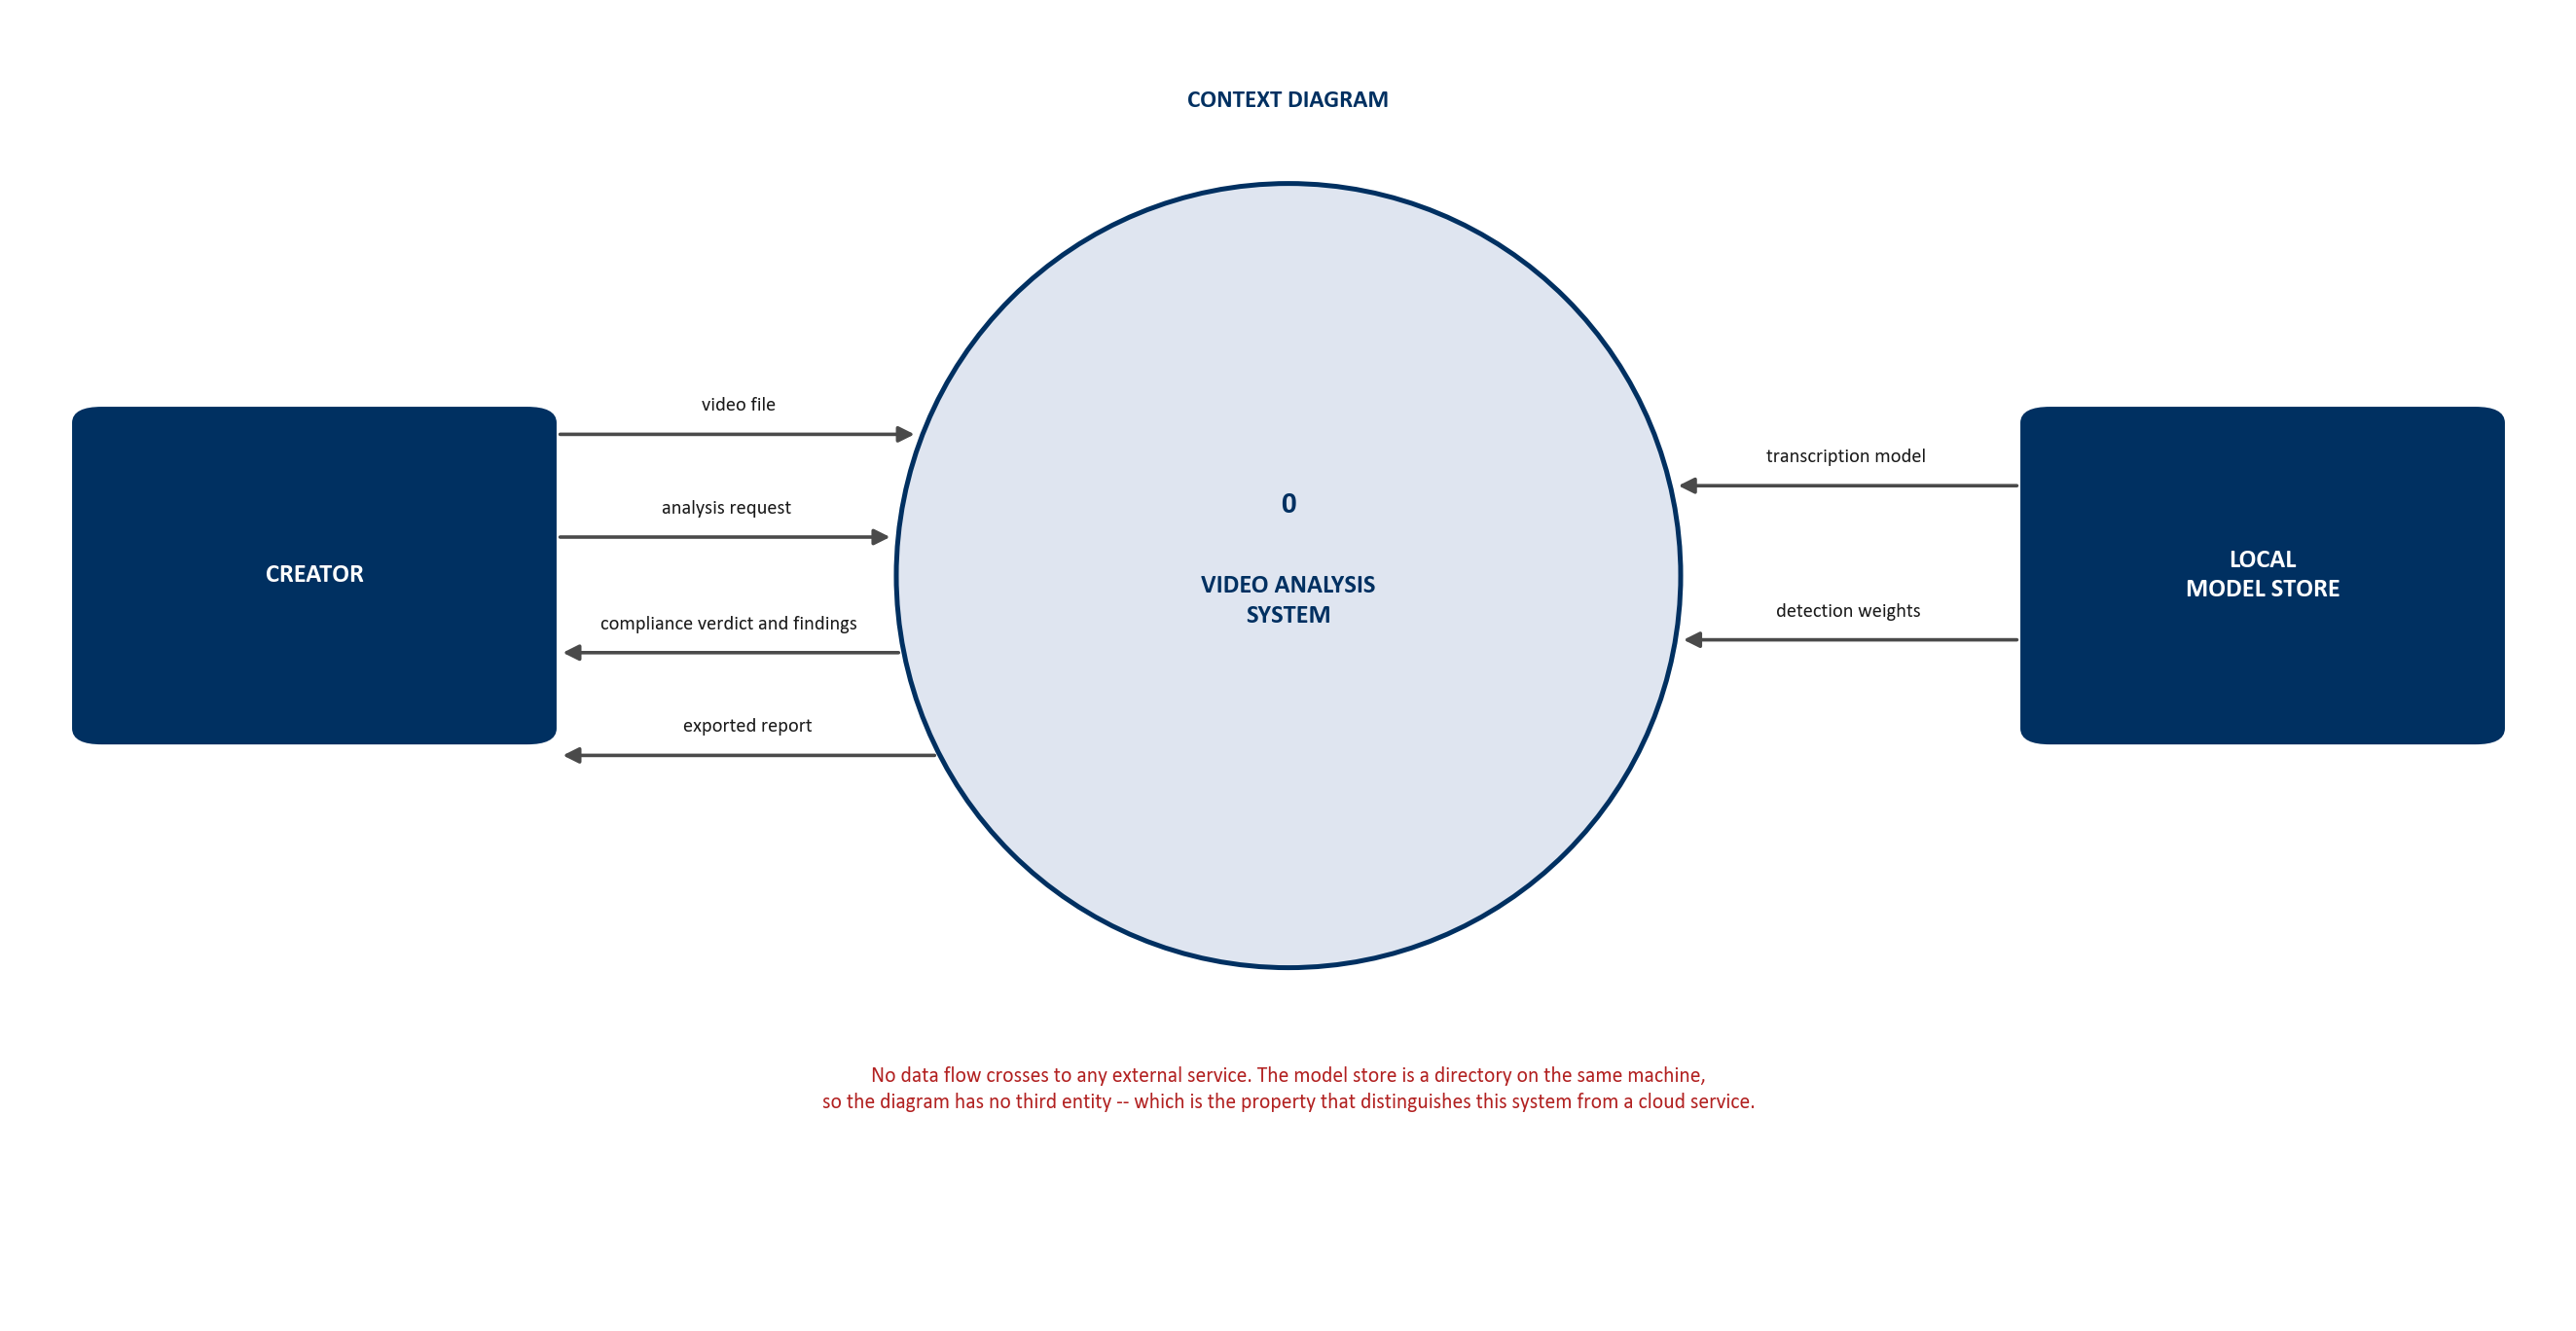
\includegraphics[width=0.92\textwidth]{Images/dfd_level0.png}
\caption{DFD Level 0}
\end{figure}

The creator supplies a video file and receives a compliance verdict, a set of
findings and an exported report. The model store supplies locally held weights.
No data flows to any external entity, which is the property that distinguishes
this system from a cloud service.

\section{Data Flow Diagram Level 1}

The Level 1 diagram decomposes the analysis system into its constituent
processes and the data stores they write to.

\begin{figure}[H]
\centering
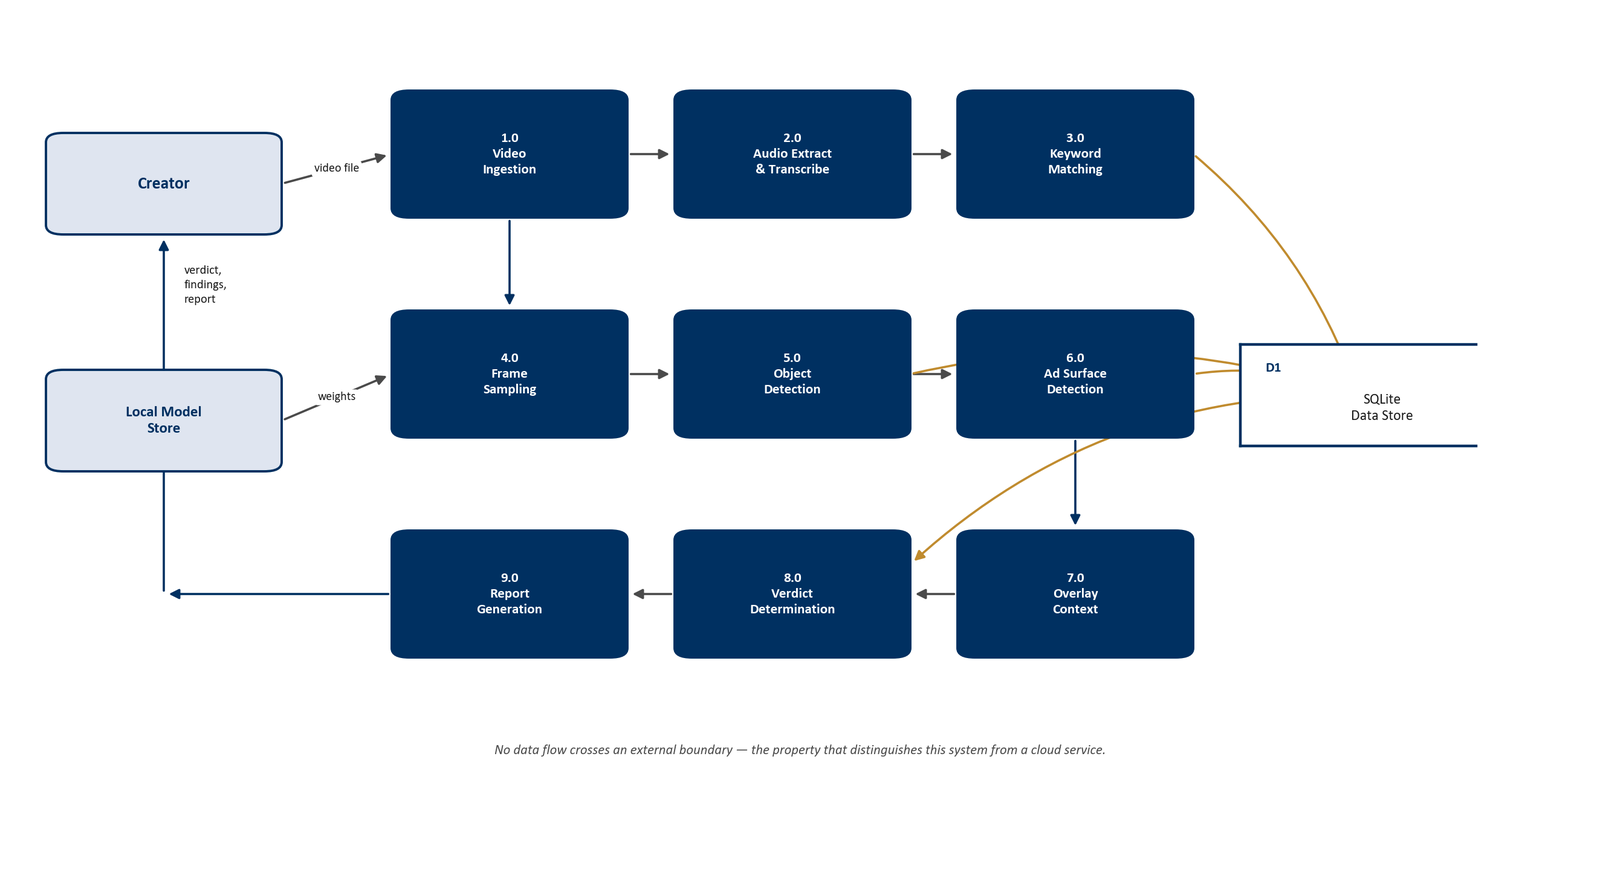
\includegraphics[width=0.95\textwidth]{Images/dfd_level1.png}
\caption{DFD Level 1}
\end{figure}

\section{Use Case Diagram}

\begin{figure}[H]
\centering
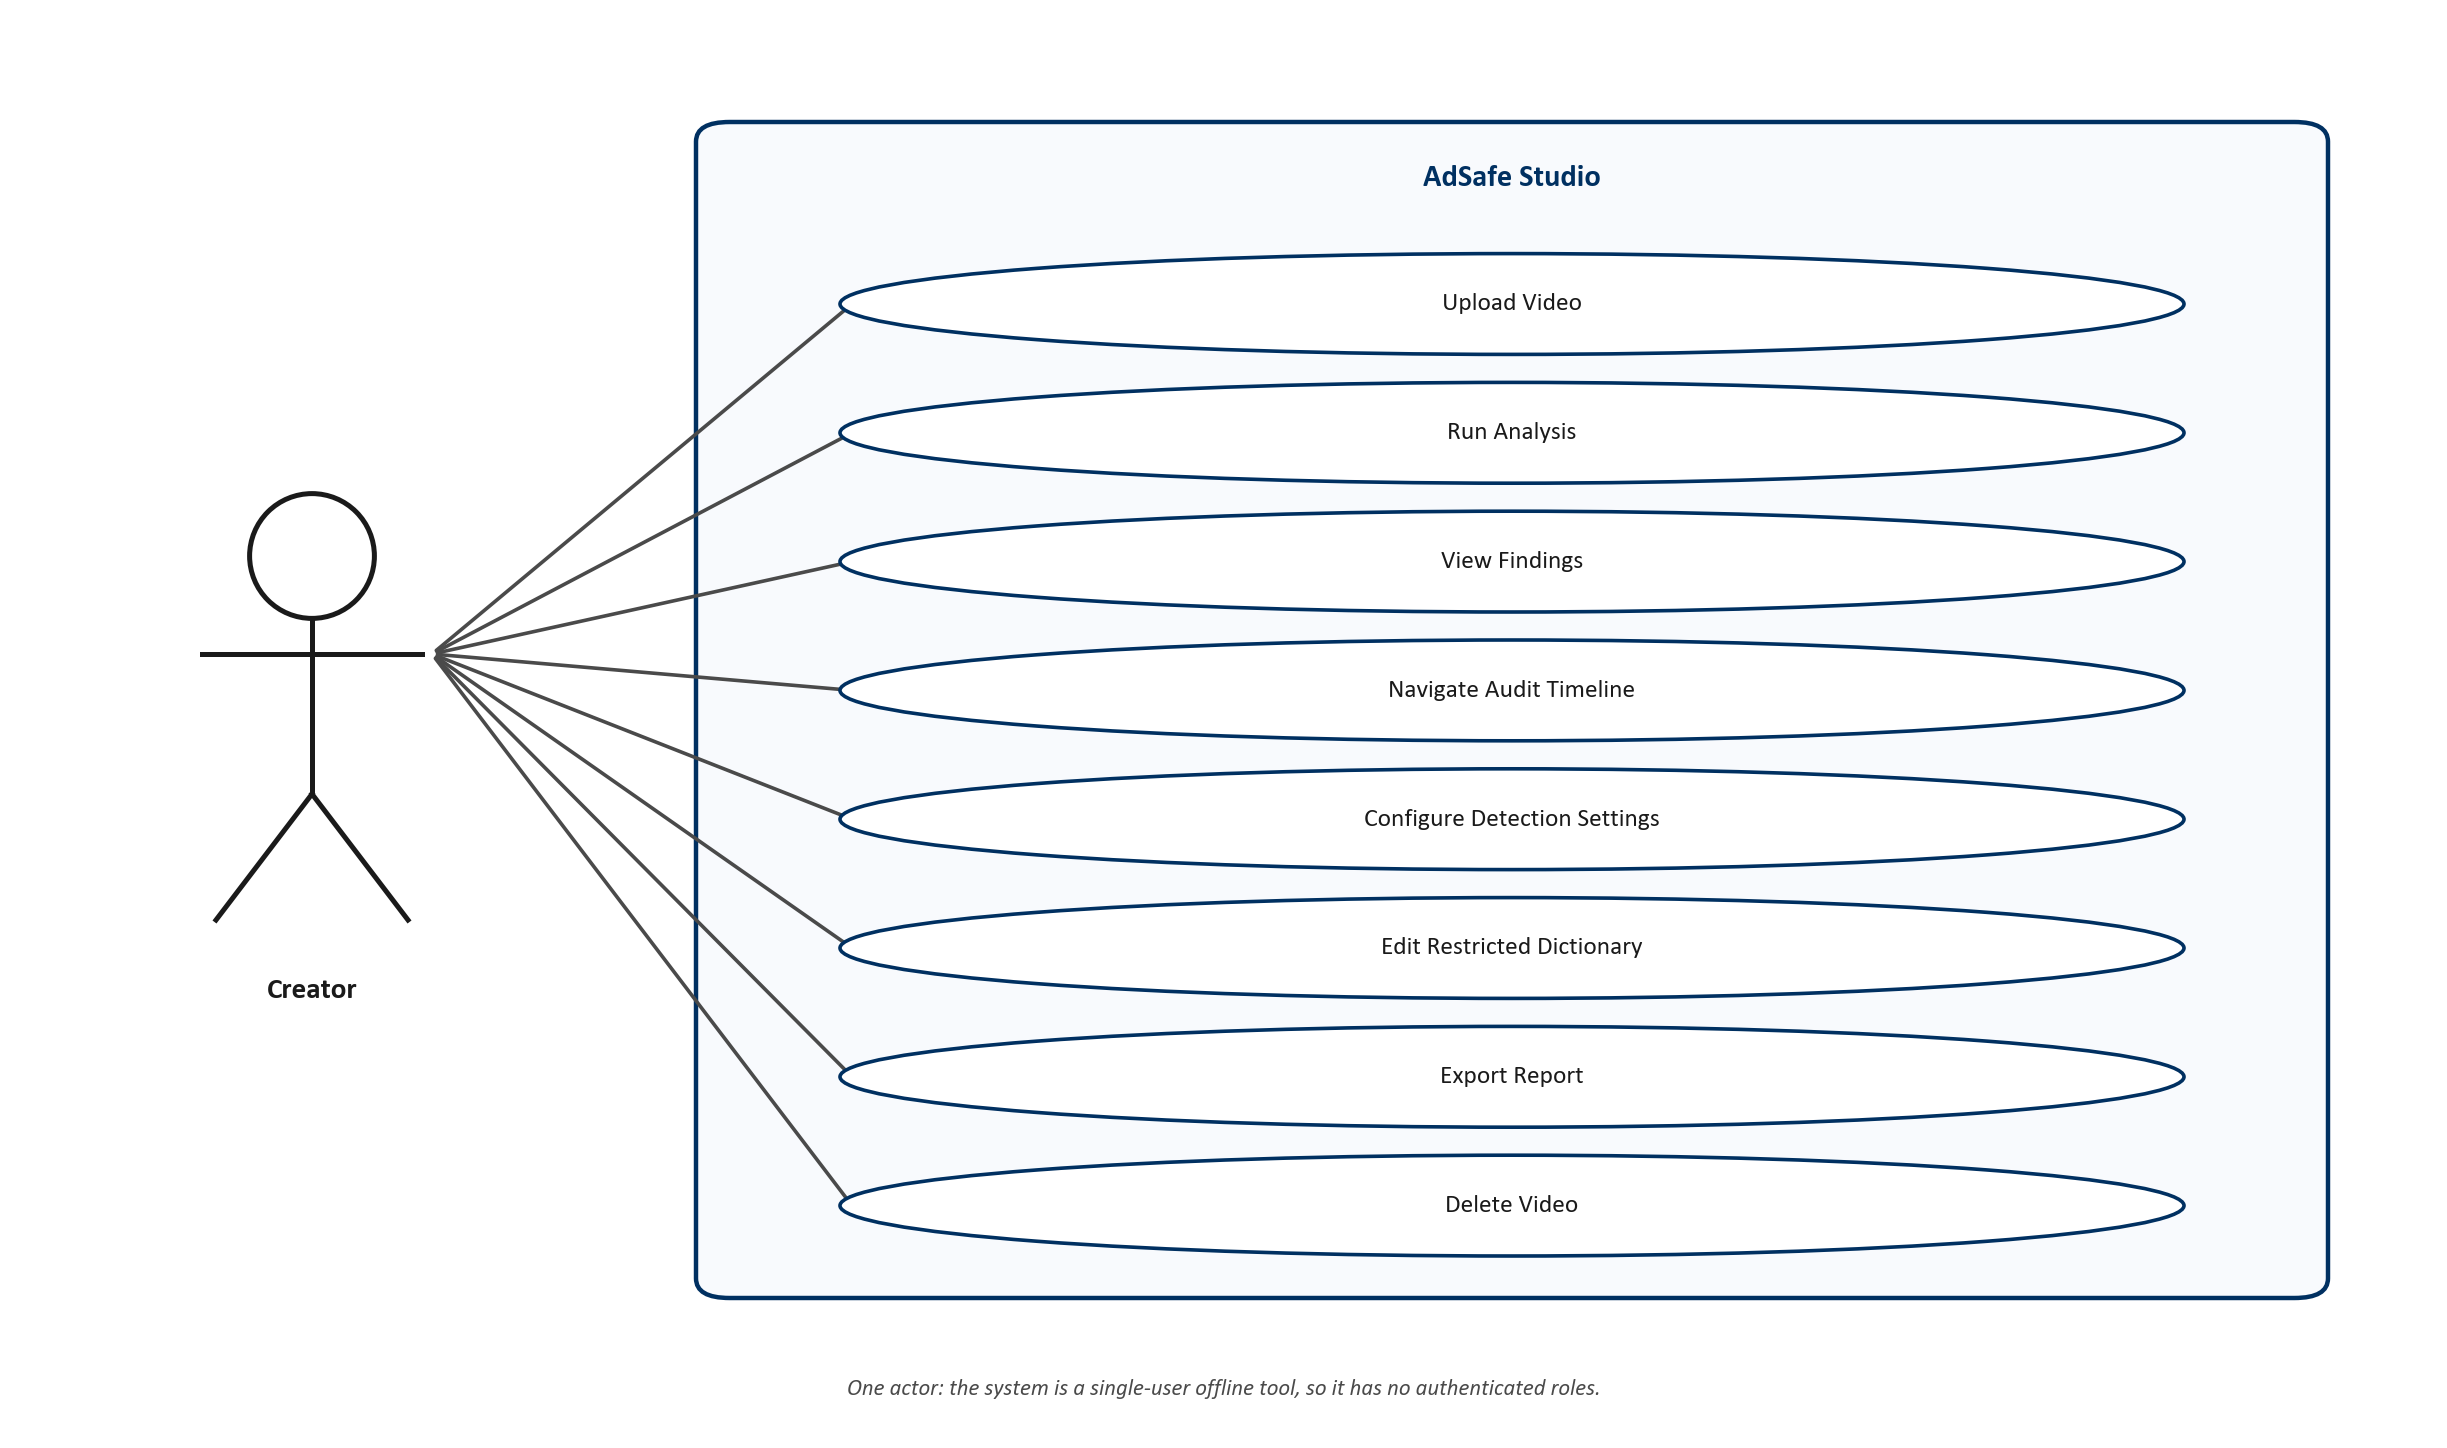
\includegraphics[width=0.92\textwidth]{Images/use_case.png}
\caption{Use Case Diagram}
\end{figure}

\section{Activity Diagram}

\begin{figure}[H]
\centering
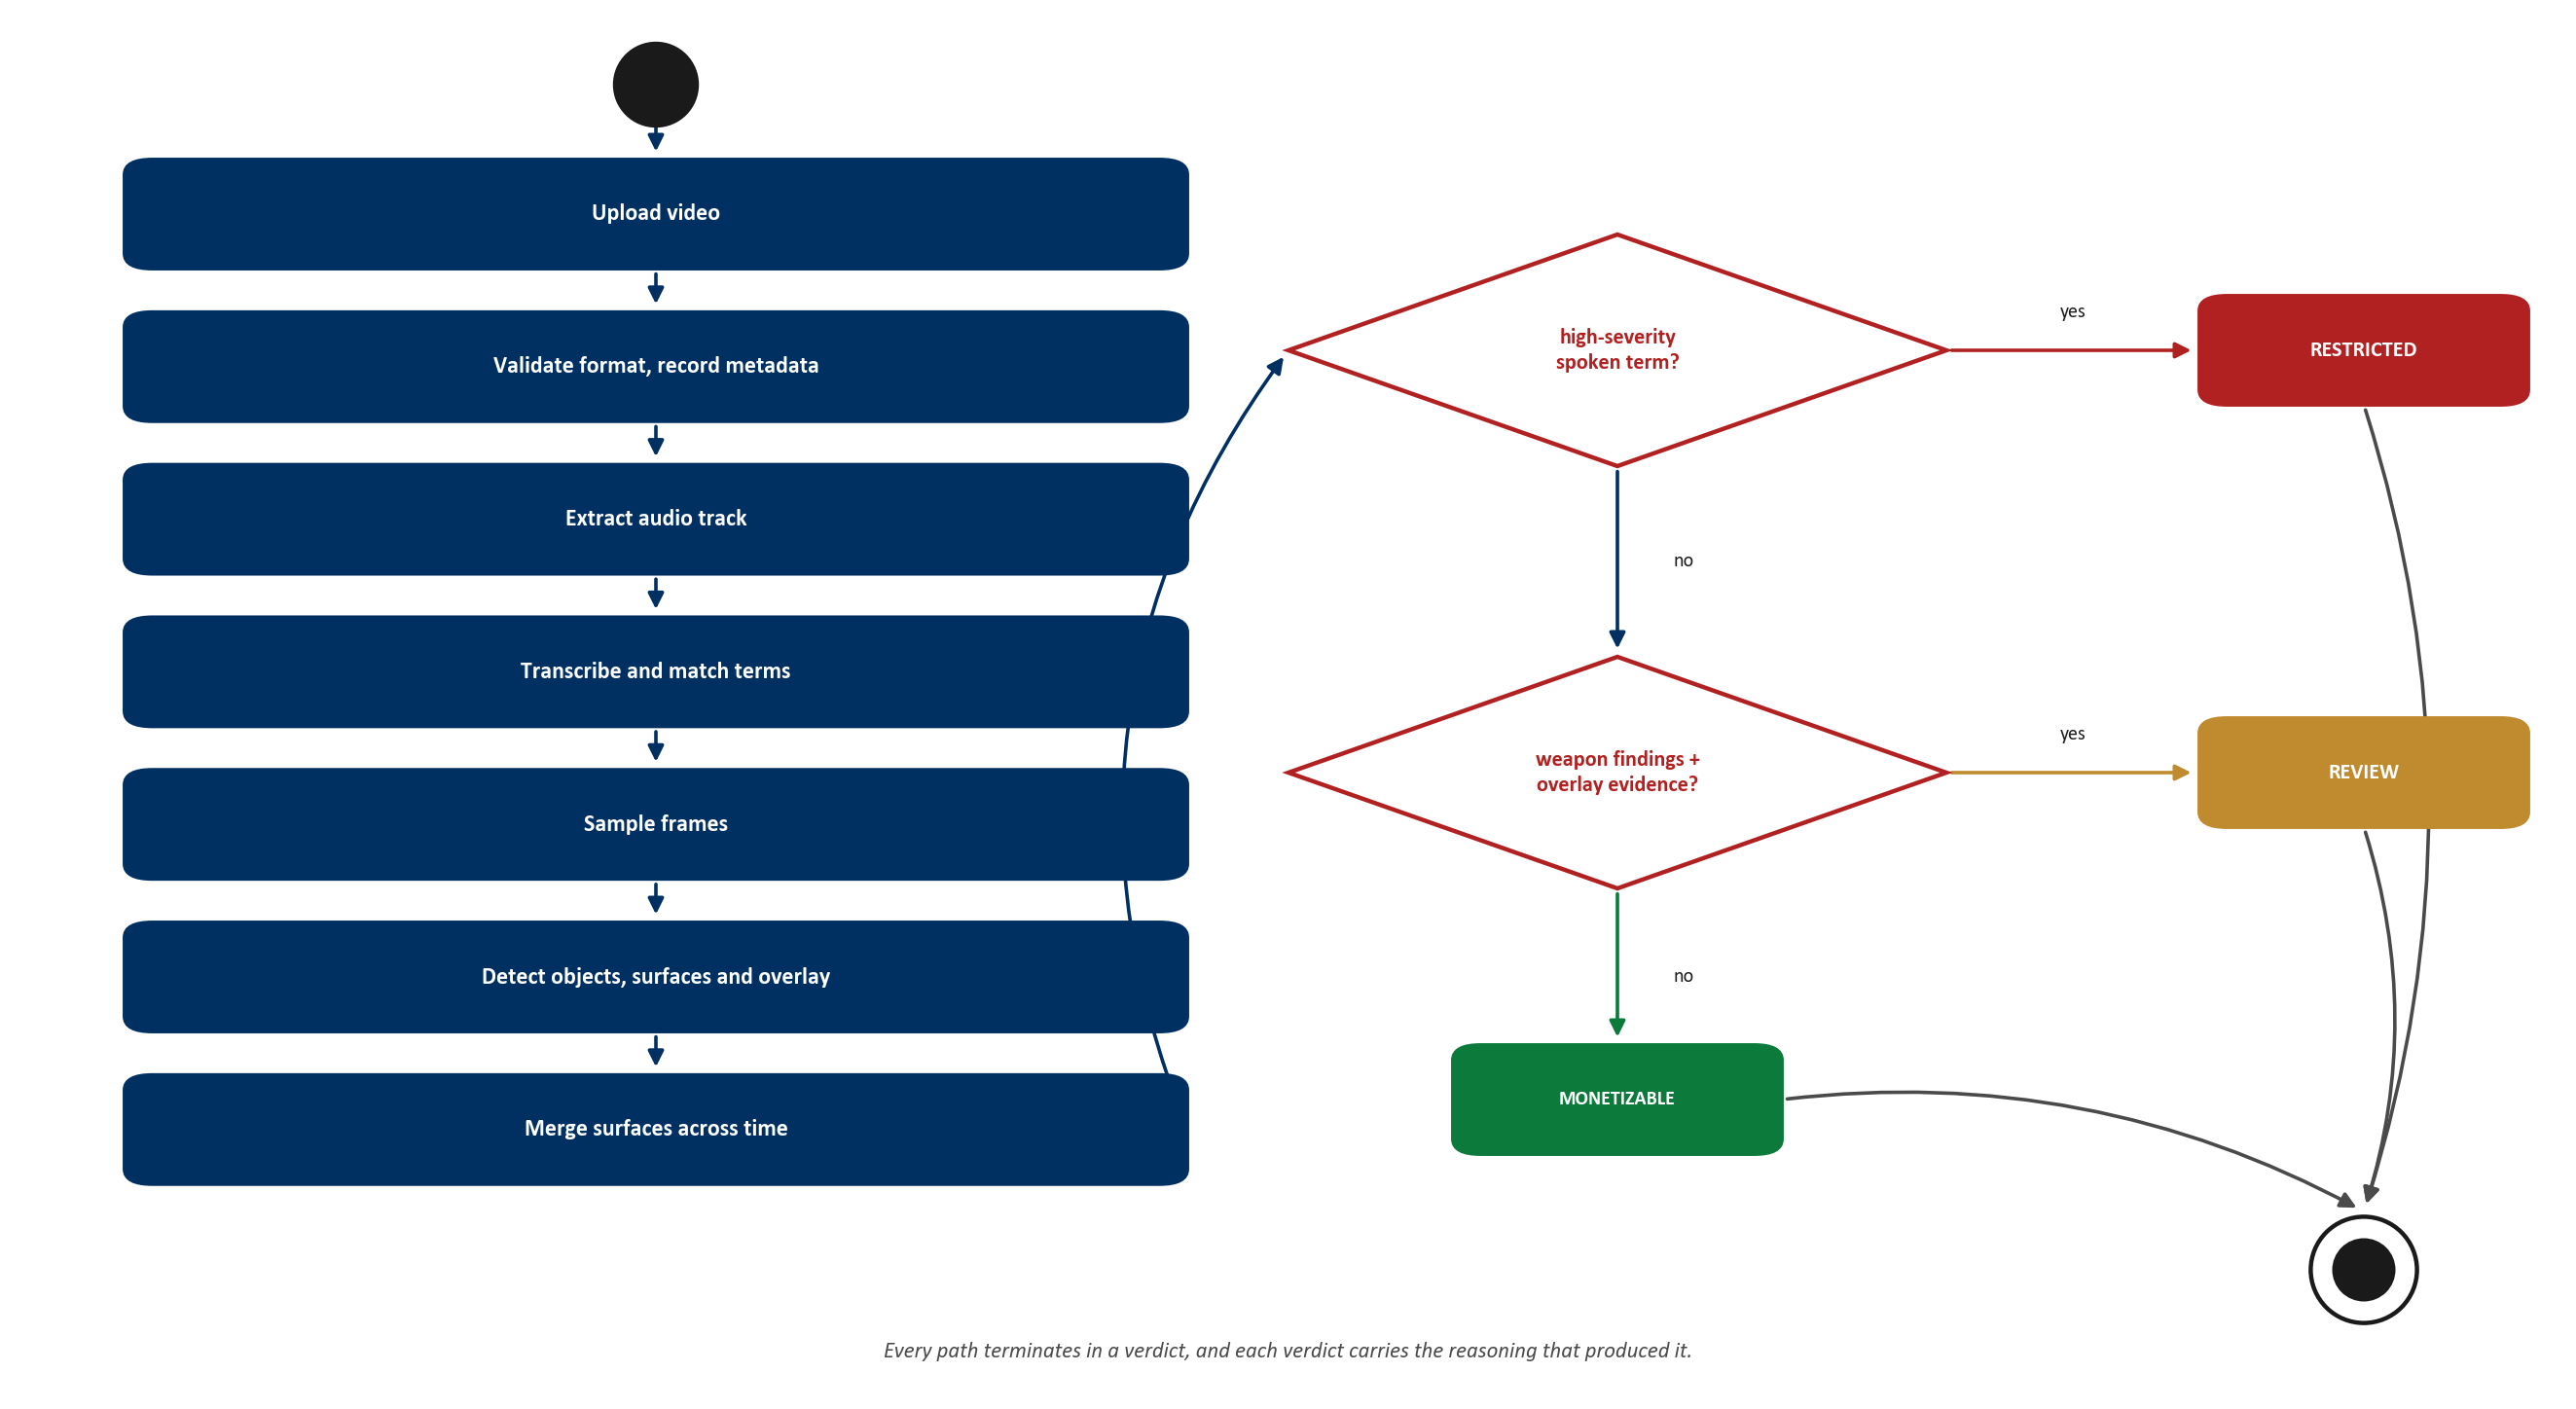
\includegraphics[width=0.88\textwidth]{Images/activity.png}
\caption{Activity Diagram}
\end{figure}

\section{Sequence Diagram}

The interface issues an analysis request to the API, which queues the work in
the background and returns immediately so the interface remains responsive. The
orchestrator invokes each engine in turn, writing findings to the database, and
reports progress that the interface polls until completion.

\begin{figure}[H]
\centering
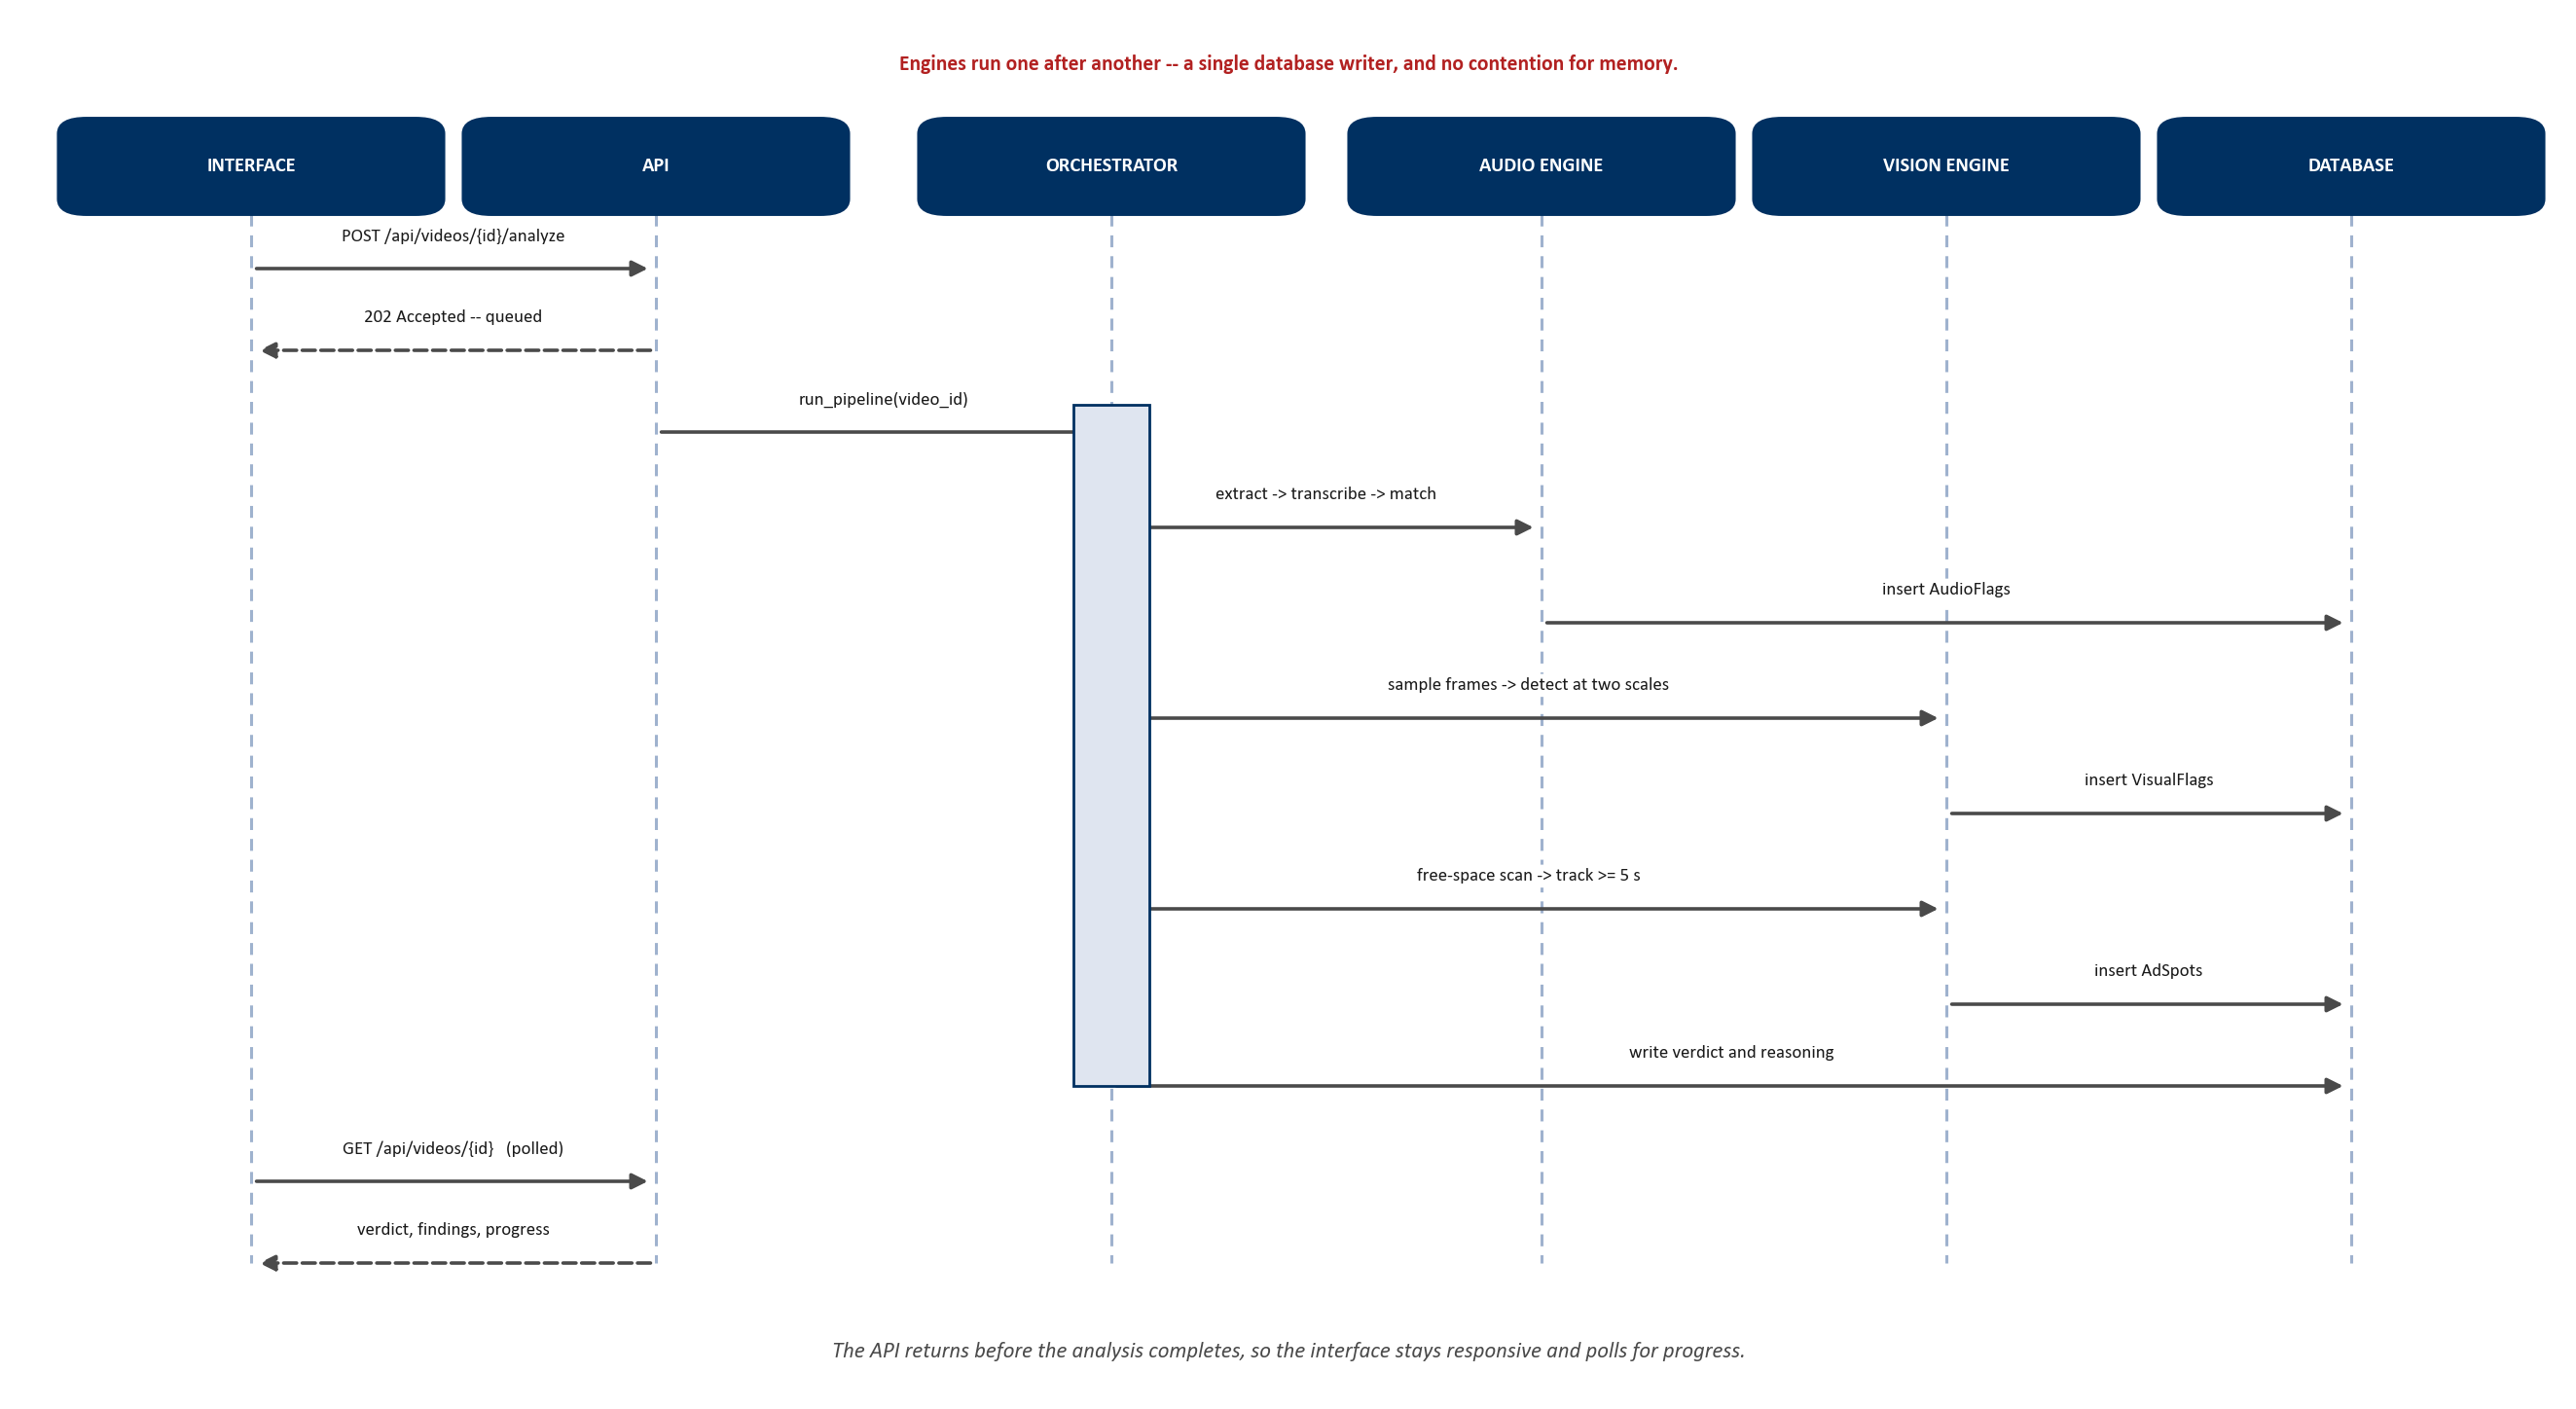
\includegraphics[width=0.95\textwidth]{Images/sequence.png}
\caption{Sequence Diagram}
\end{figure}

\section{State Diagram}

A video record moves through exactly four states, constrained by a database
check constraint rather than by convention alone.

\begin{figure}[H]
\centering
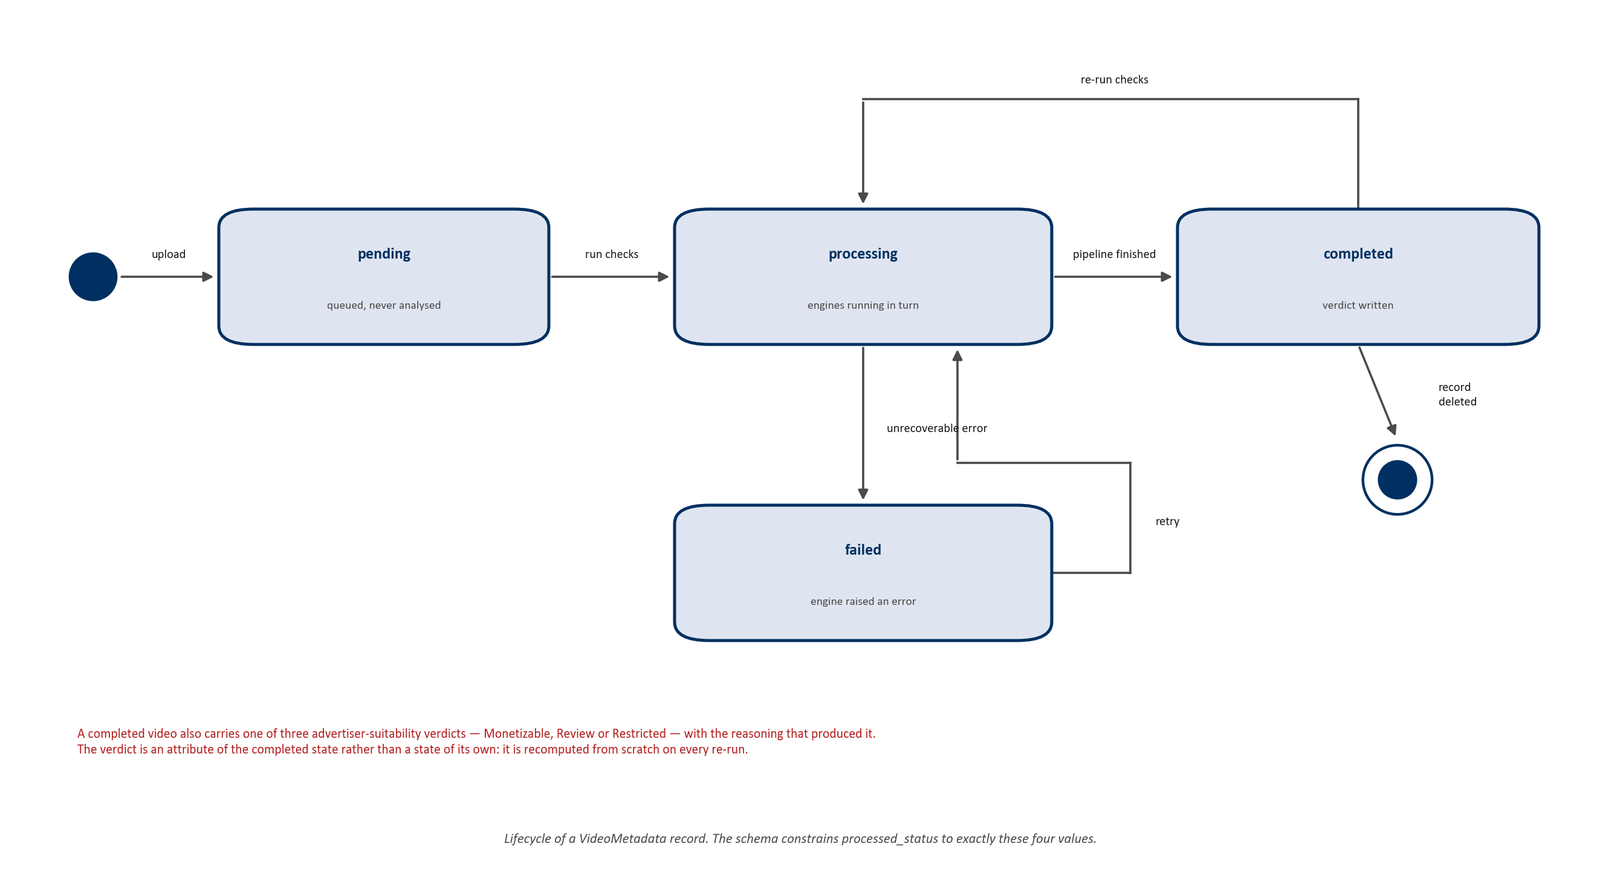
\includegraphics[width=0.95\textwidth]{Images/state_diagram.png}
\caption{State Diagram}
\end{figure}

\section{Class Diagram}

\begin{figure}[H]
\centering
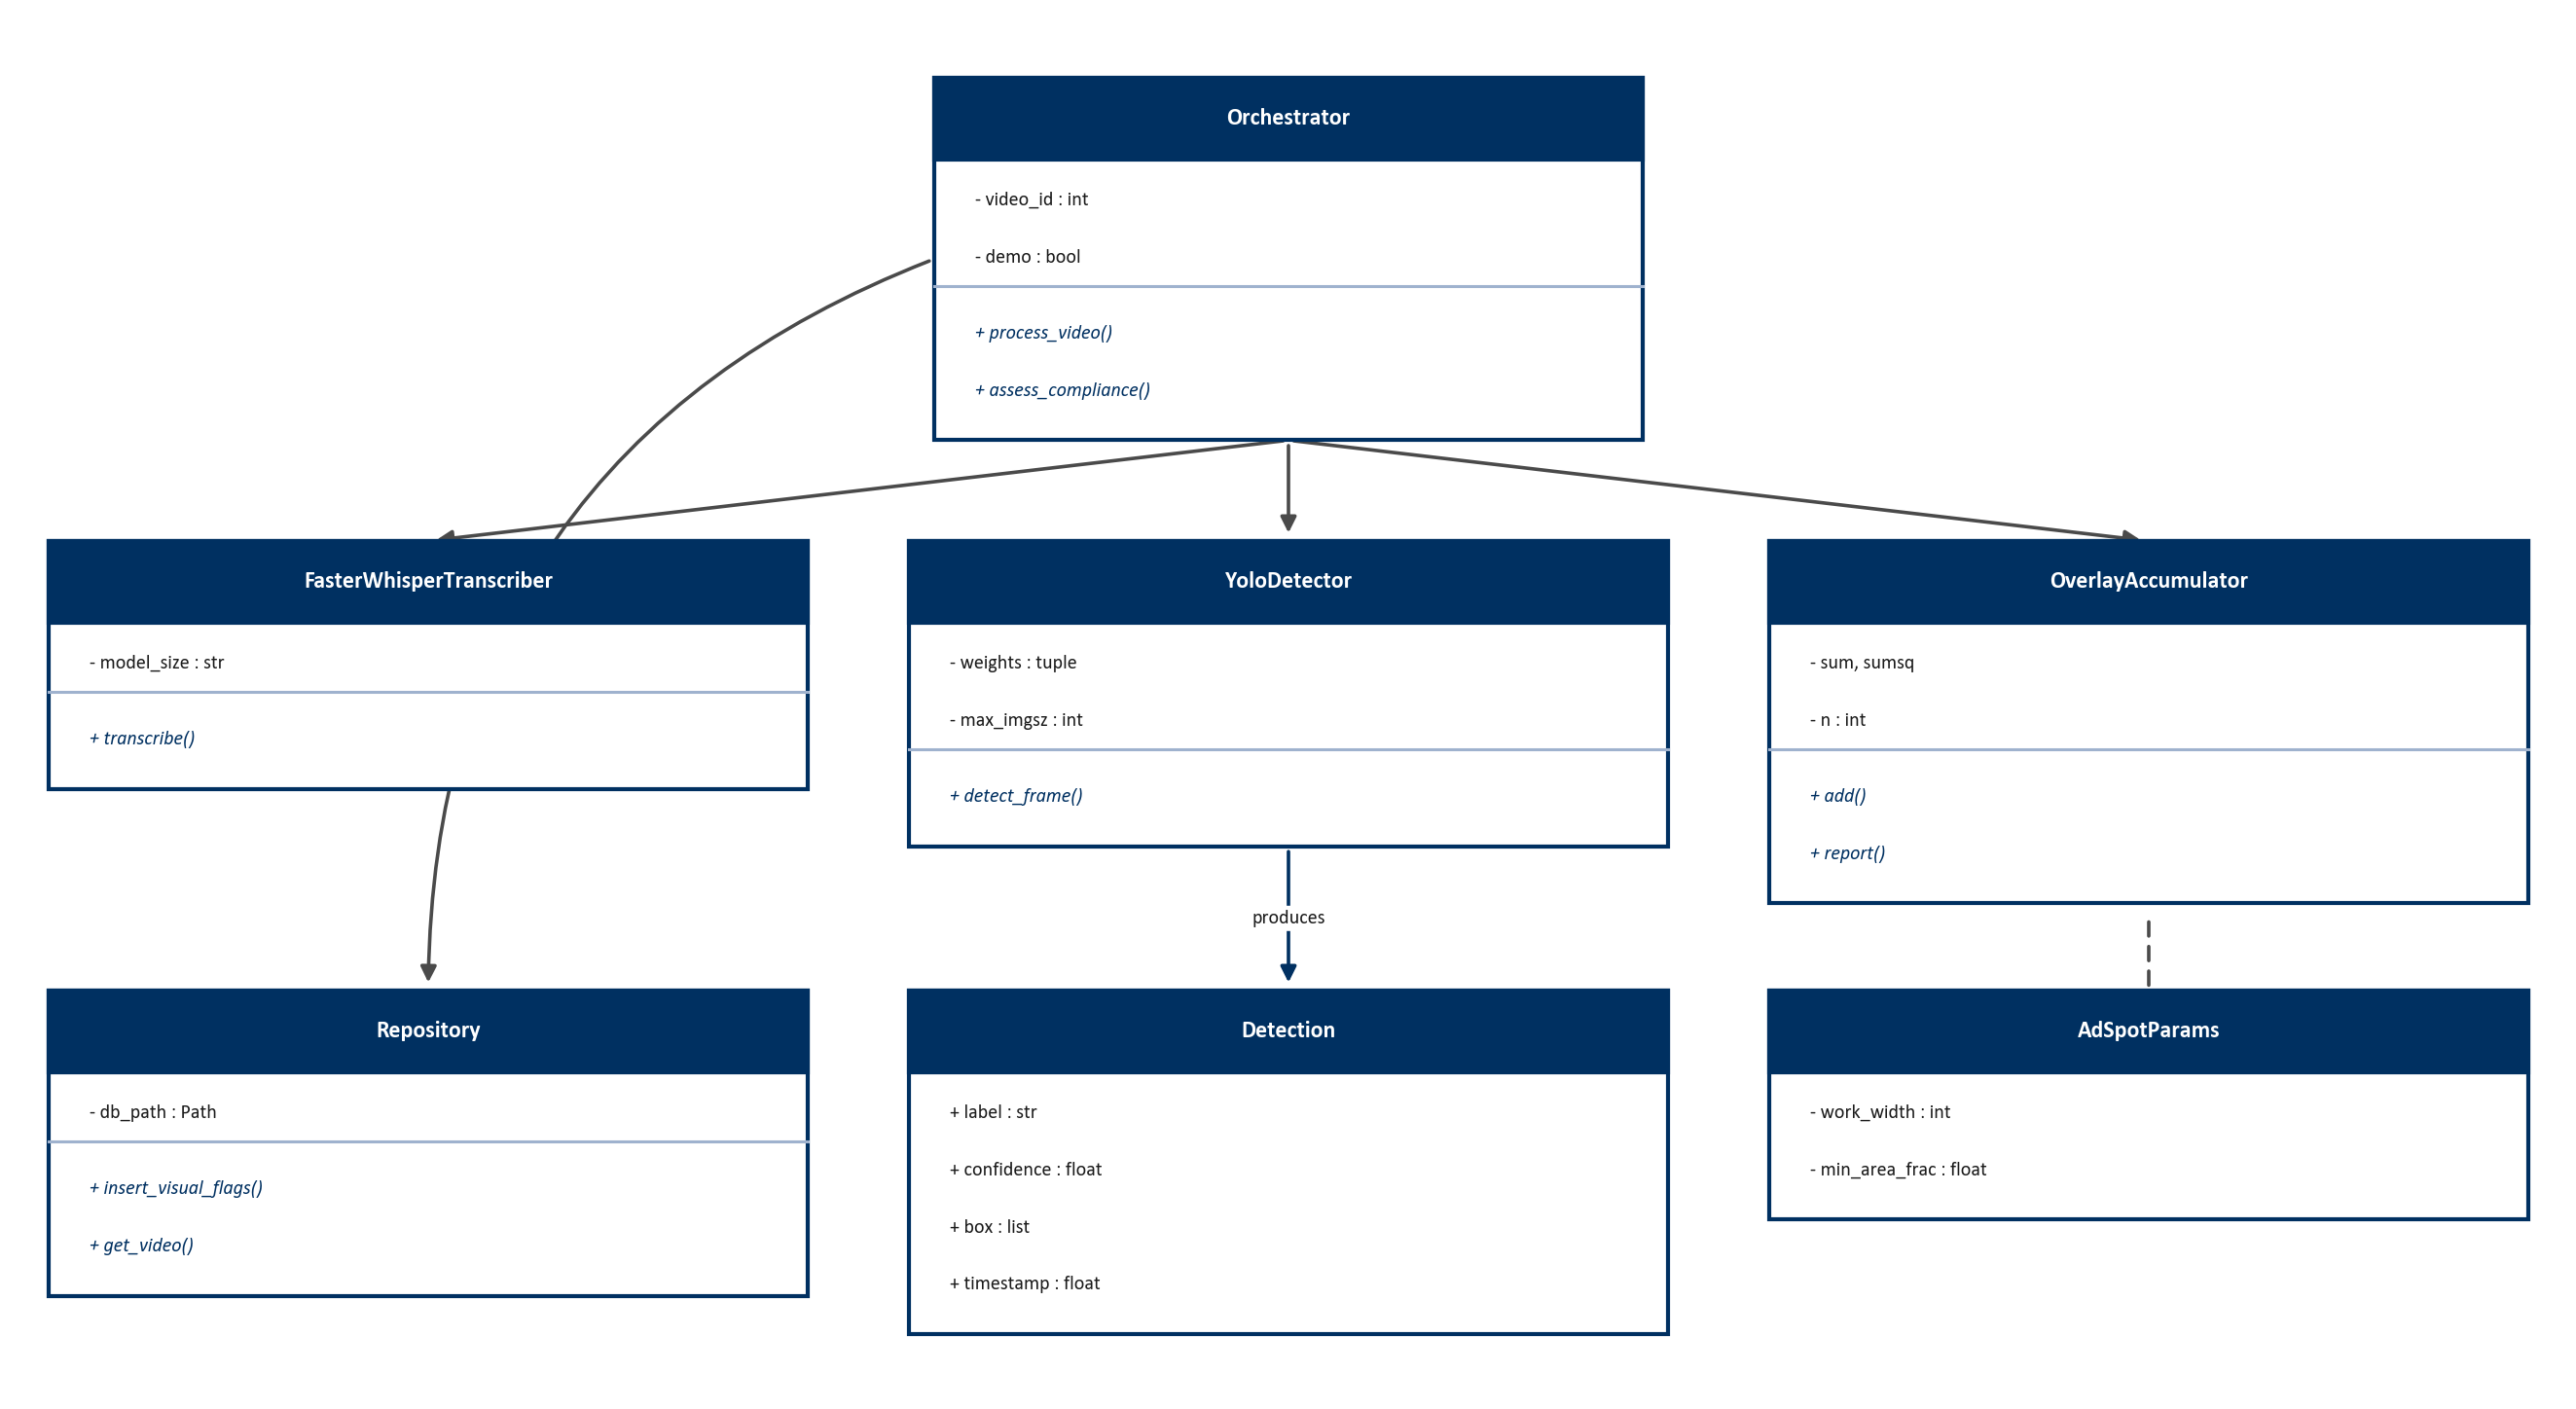
\includegraphics[width=0.95\textwidth]{Images/class_diagram.png}
\caption{Class Diagram}
\end{figure}

\section{Entity Relationship Diagram}

\begin{figure}[H]
\centering
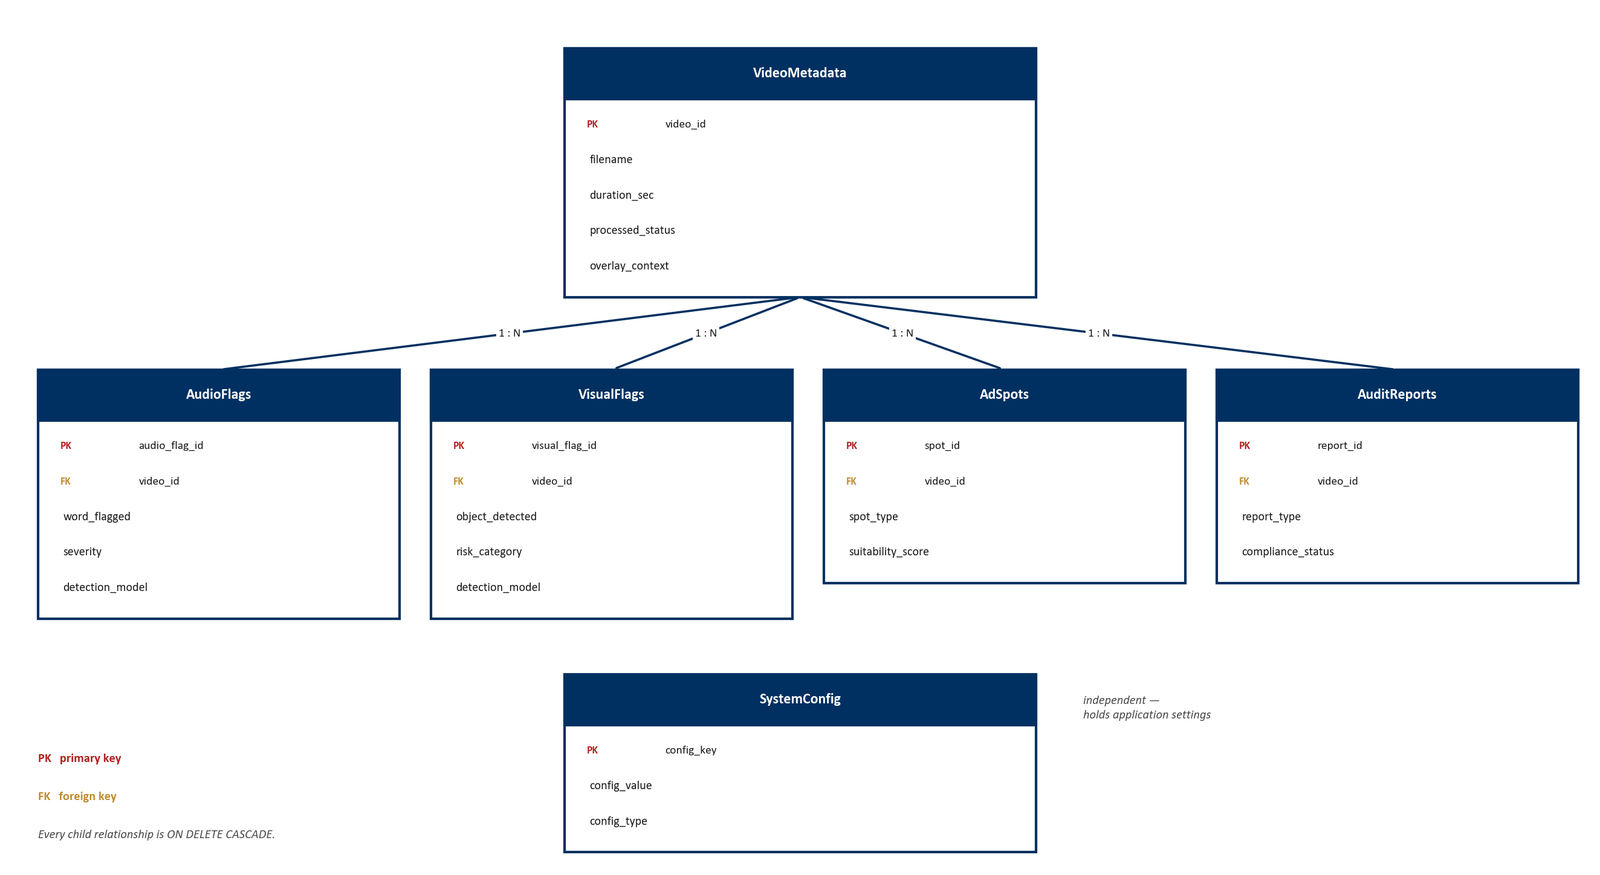
\includegraphics[width=0.95\textwidth]{Images/er_diagram.png}
\caption{Entity Relationship Diagram}
\end{figure}

\section{Control Flow Diagram}

The control flow diagram shows the order in which the engines execute within a
single analysis, including the branch taken when a video carries no audio track.

\begin{figure}[H]
\centering
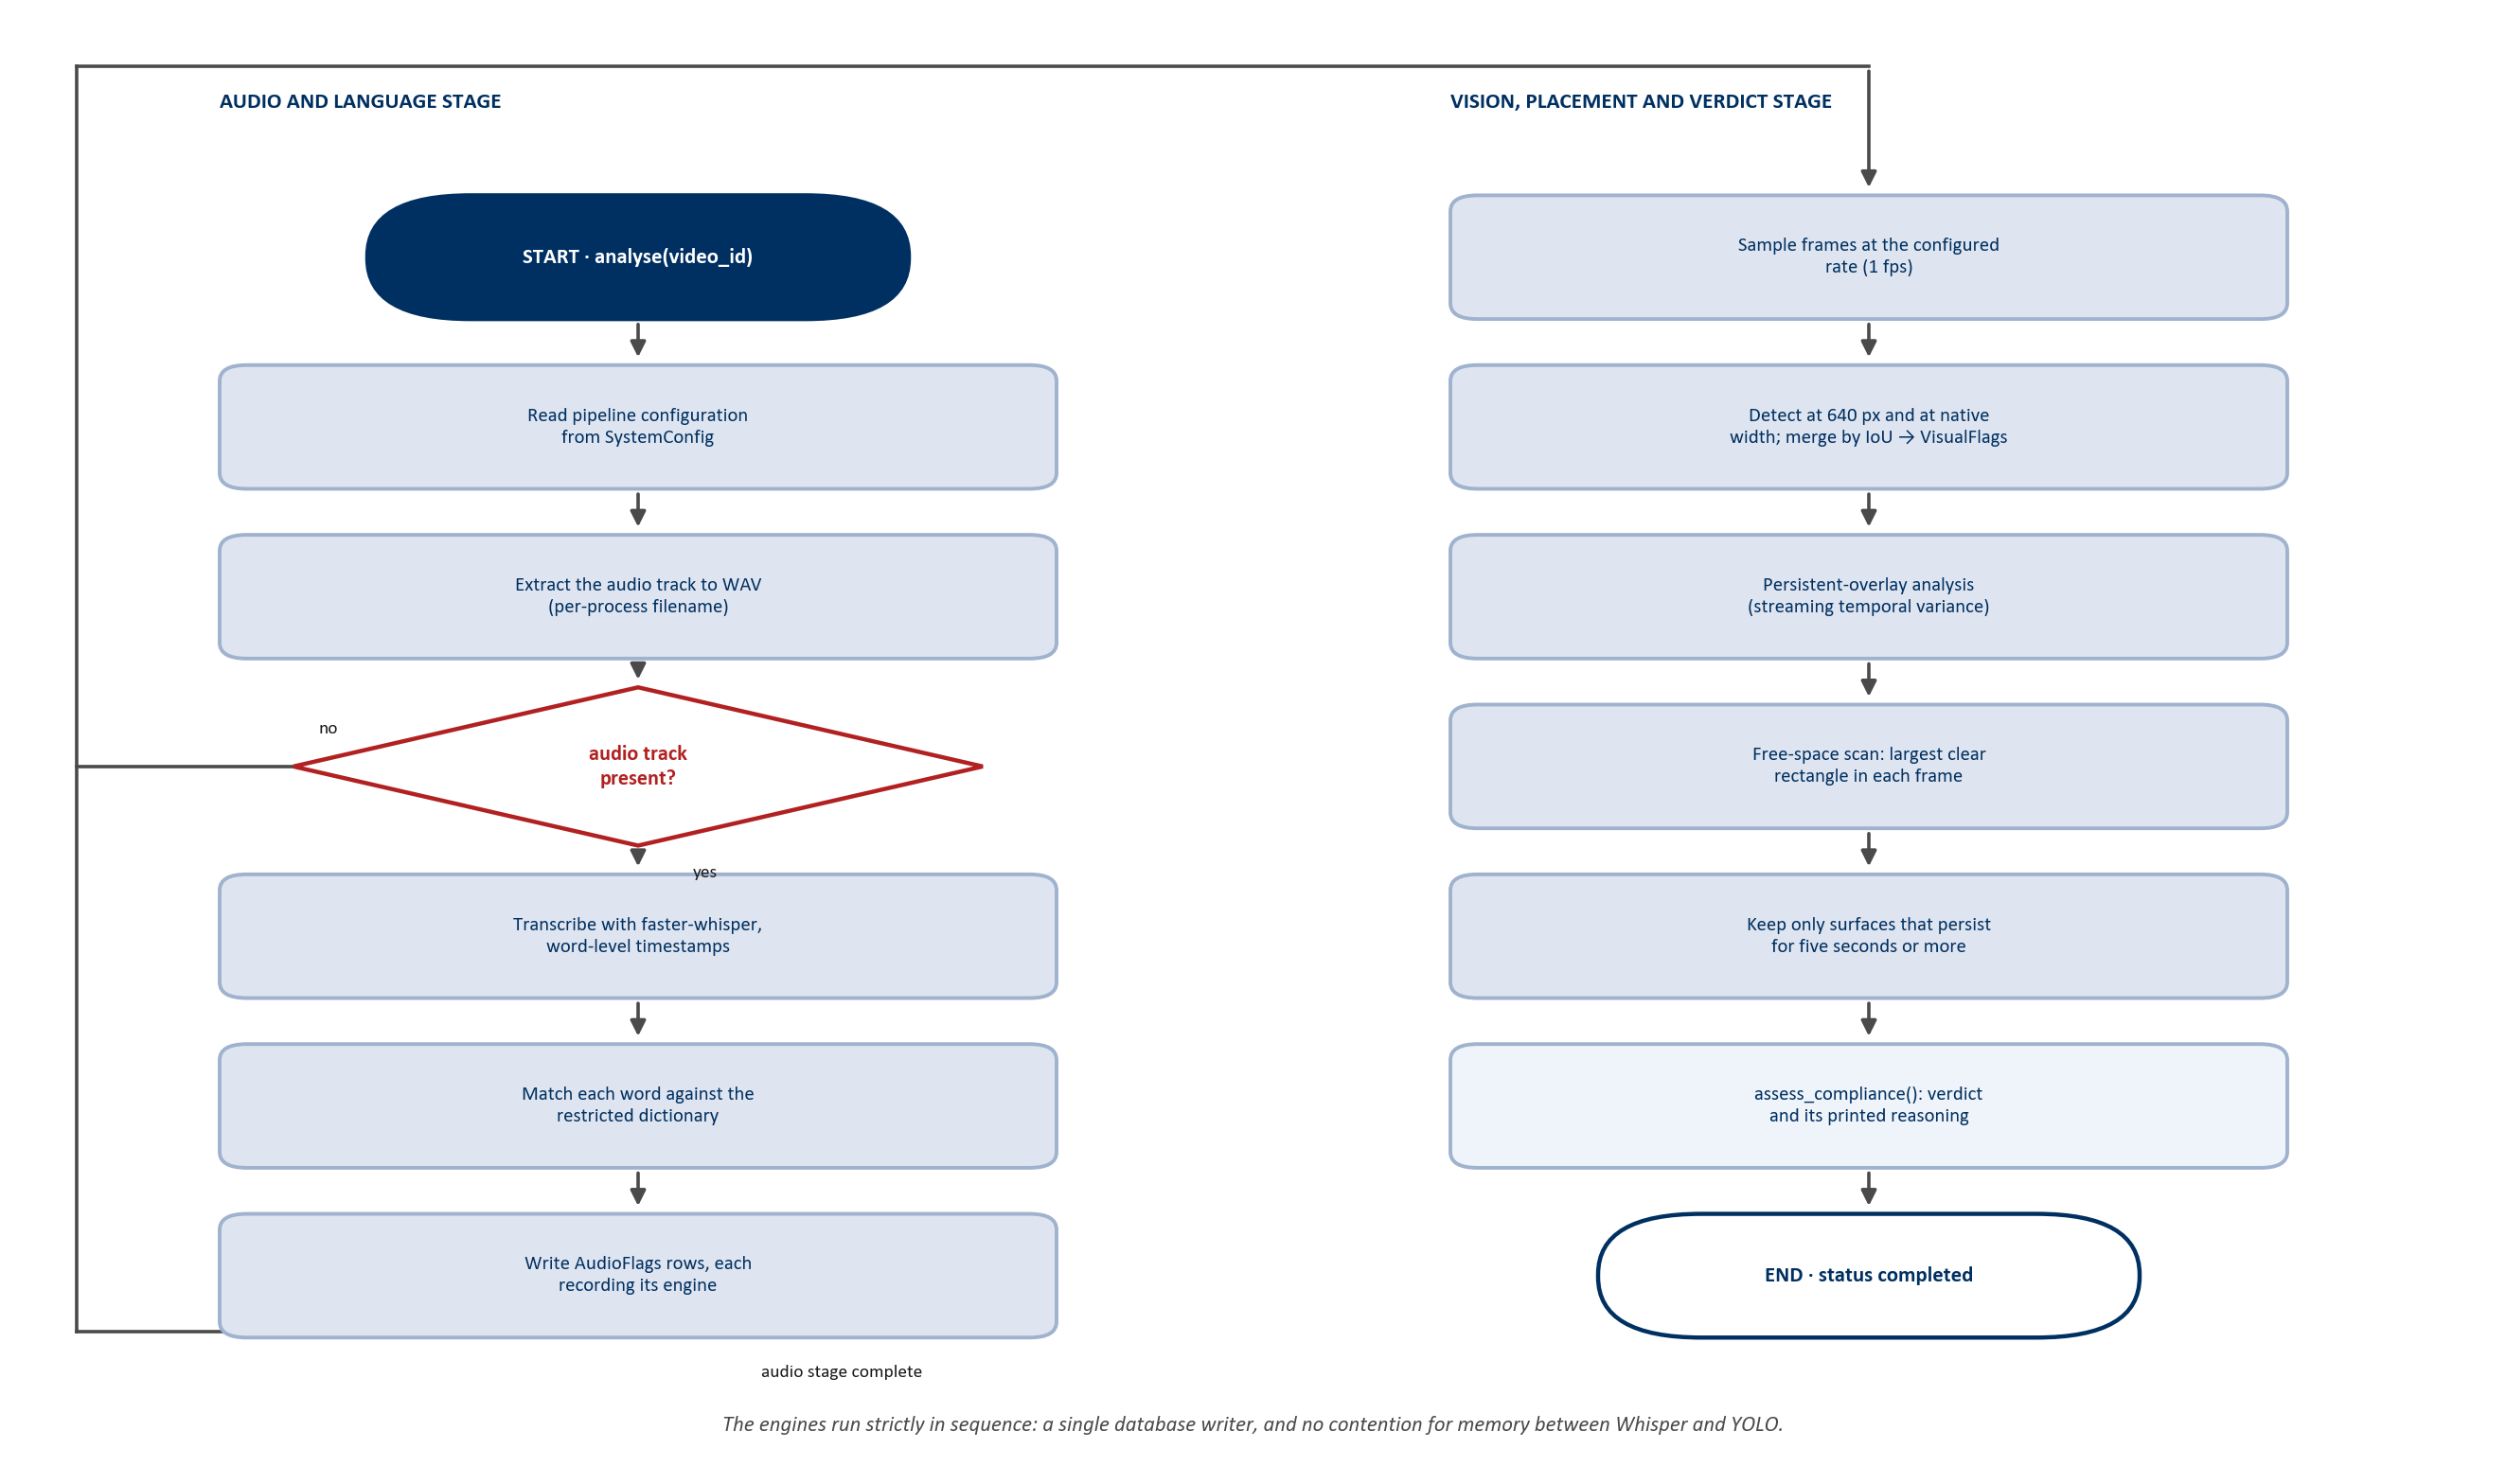
\includegraphics[width=0.95\textwidth]{Images/control_flow.png}
\caption{Control Flow Diagram}
\end{figure}

%%%%%%%%%%%%%%%%%%%%%%%%%%%%%%%%%%%%%%%%%%%%%%%%%%
\chapter{System Design}
%%%%%%%%%%%%%%%%%%%%%%%%%%%%%%%%%%%%%%%%%%%%%%%%%%

\section{Introduction}

This chapter describes the architecture of the system, the decomposition into
modules, the database design and its constraints, and the design of the user
interface.

\section{System Architecture}

The system follows a four-layer architecture: presentation, controller, AI
engine and data \cite{Martin2017}.

\begin{figure}[H]
\centering
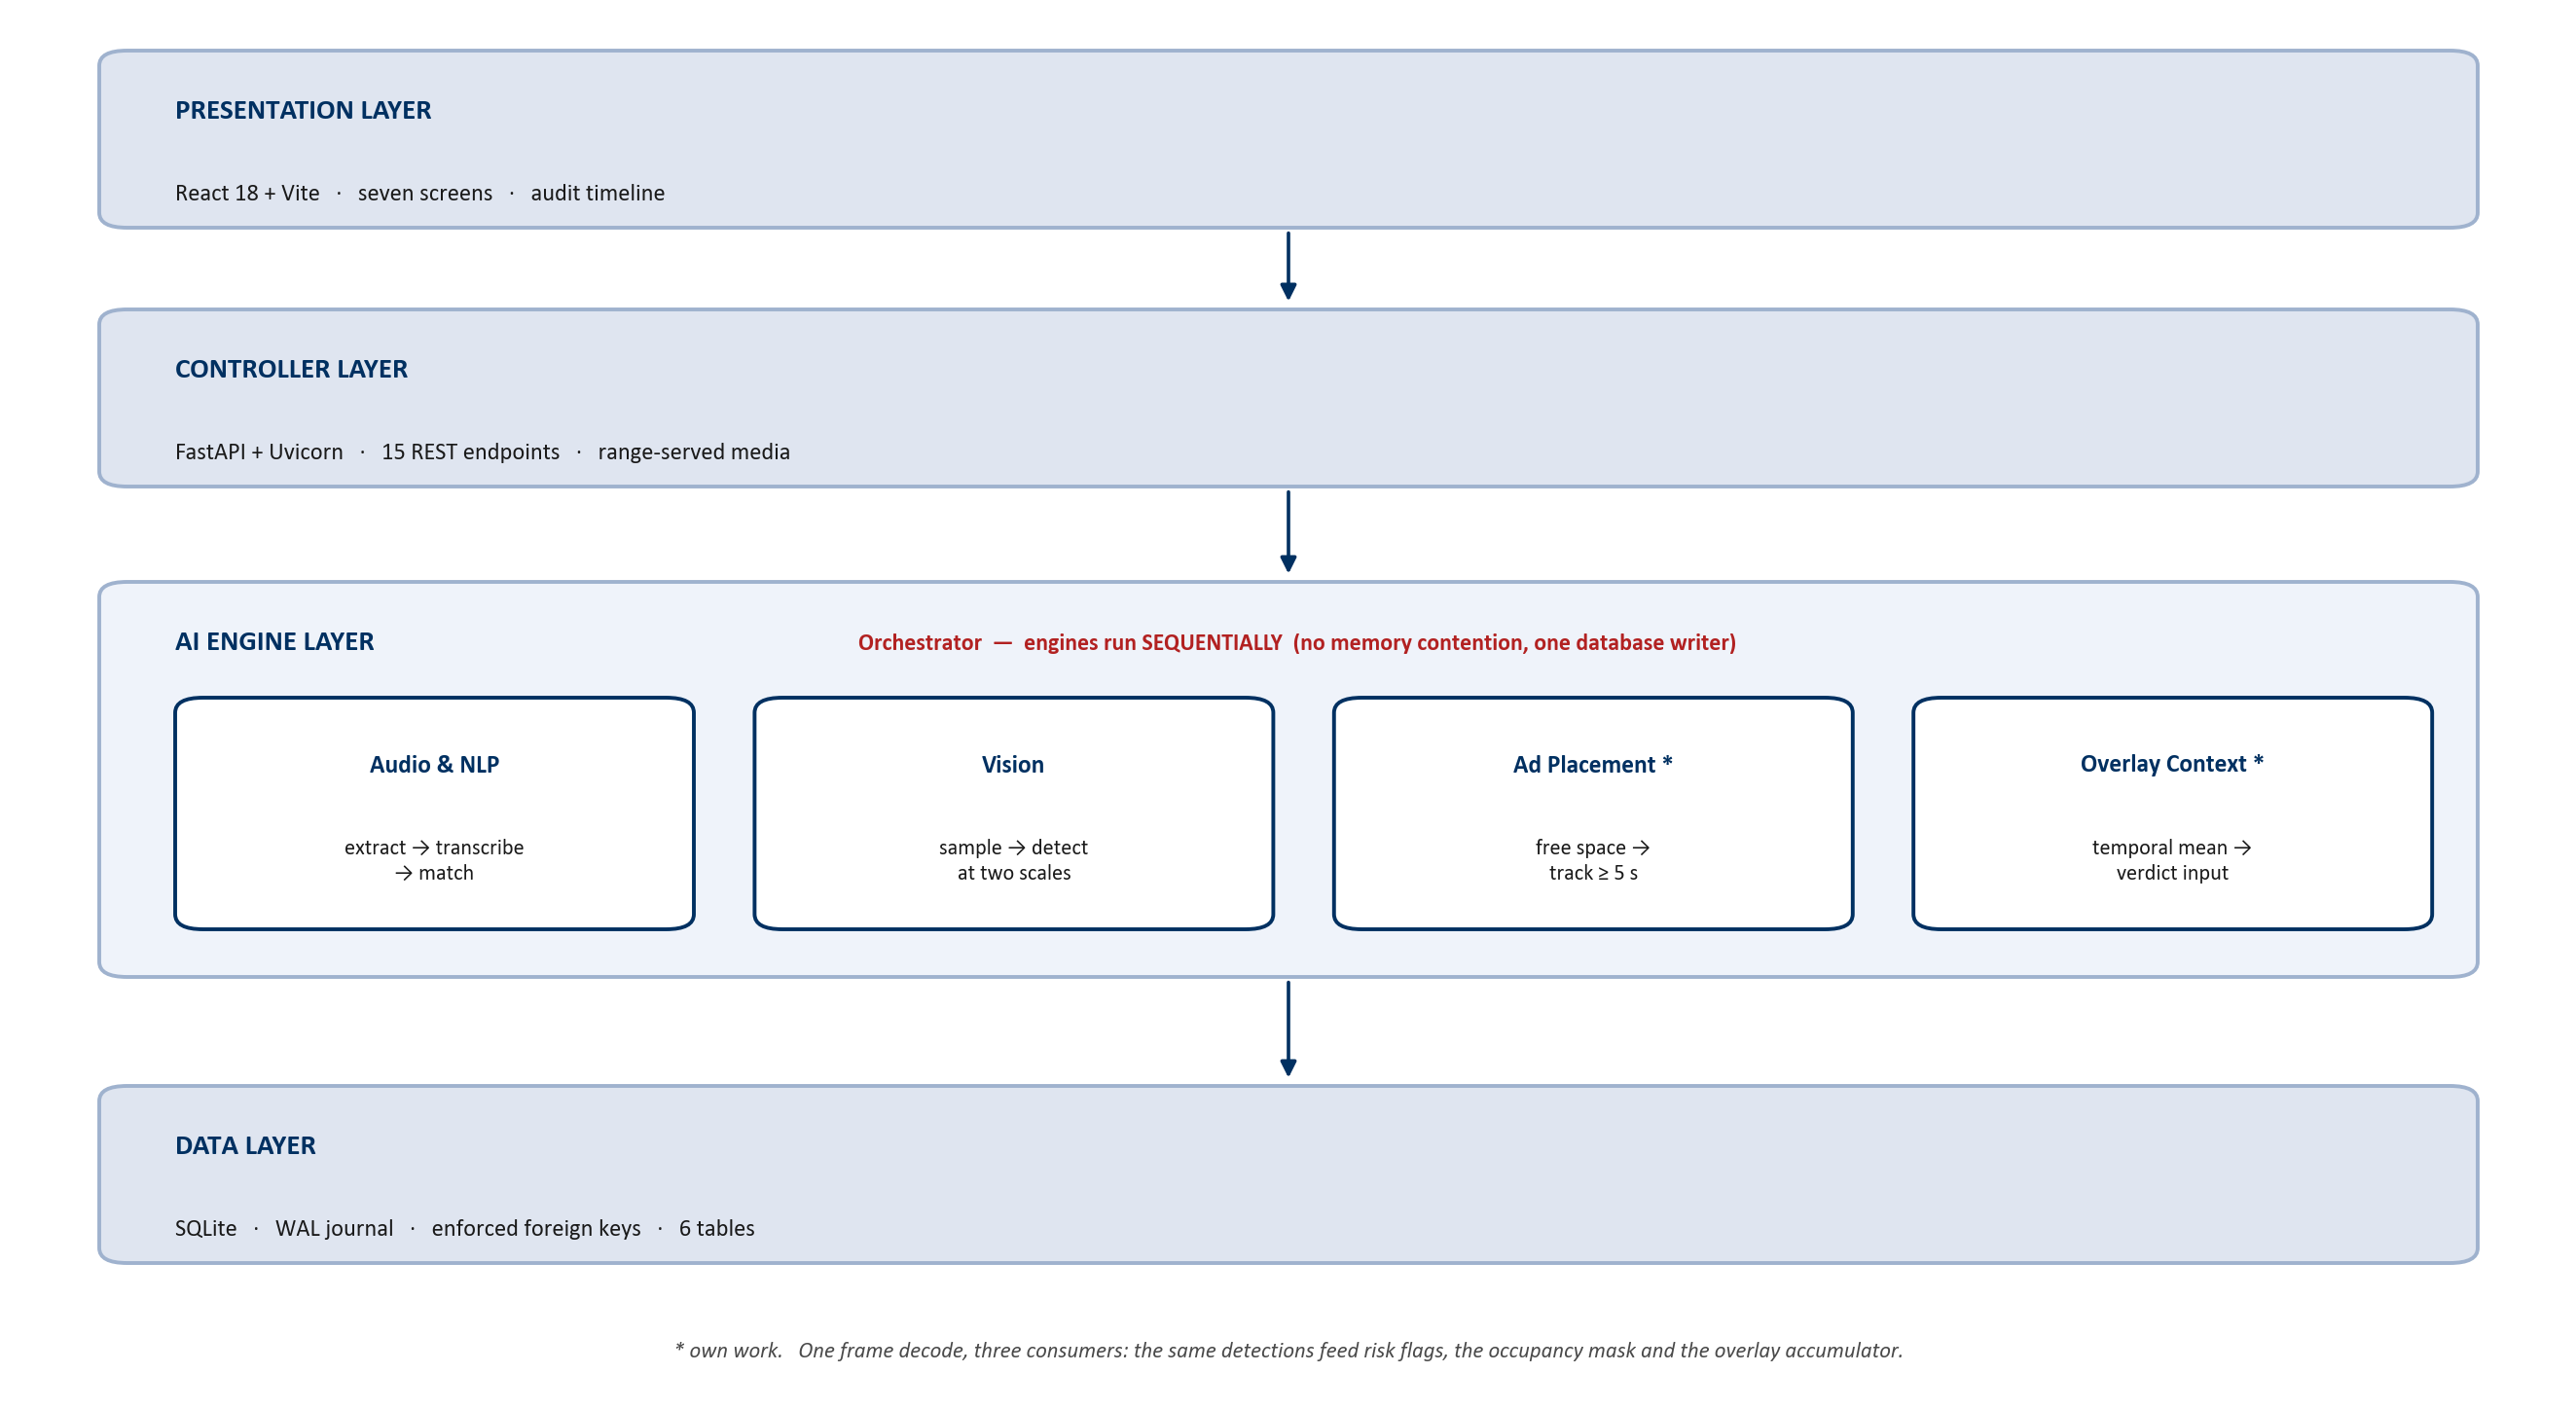
\includegraphics[width=0.95\textwidth]{Images/architecture.png}
\caption{System Architecture}
\end{figure}

The decisive property of this architecture is that \textbf{the engines run
sequentially, not in parallel}. Two documents produced earlier in the project
disagreed on this point; sequential execution is correct and is what was built,
for three reasons. Whisper and YOLO contend for the same memory. Python's global
interpreter lock limits true parallelism for this workload in any case. And
concurrent writers against SQLite produce lock errors. A single writer, running
one engine at a time, avoids all three.

\section{Modularization Details}

\begin{table}[H]
\centering
\begin{tabular}{|p{4cm}|p{9cm}|}
\hline
\textbf{Module} & \textbf{Responsibility} \\
\hline
\texttt{src/audio} & Audio extraction to WAV, transcription with word-level
timestamps, restricted-vocabulary matching and severity assignment \\
\hline
\texttt{src/vision} & Frame sampling, multi-scale object detection and merging,
persistent-overlay analysis, free-space surface detection, surface tracking \\
\hline
\texttt{src/pipeline} & Orchestration of the engines in sequence, progress
reporting, and computation of the compliance verdict \\
\hline
\texttt{src/db} & Connection management, schema creation, migrations, seeding
and all query access \\
\hline
\texttt{src/reports} & PDF, CSV and JSON export of audit findings \\
\hline
\texttt{src/benchmark} & Clip intake, labelling support, evaluation and coverage
gating \\
\hline
\texttt{backend} & FastAPI application, 15 REST endpoints, background task
scheduling, range-served media \\
\hline
\texttt{frontend} & React single-page application, seven screens, audit timeline
component \\
\hline
\end{tabular}
\caption{Module Description}
\end{table}

\section{Data Integrity and Constraints}

\subsection{Primary Key Constraints}

Every table has an integer surrogate primary key declared \texttt{INTEGER
PRIMARY KEY AUTOINCREMENT}, with the single exception of \texttt{SystemConfig},
whose primary key is the natural key \texttt{config\_key}.

\subsection{Foreign Key Constraints}

Each of \texttt{AudioFlags}, \texttt{VisualFlags}, \texttt{AdSpots} and
\texttt{AuditReports} holds \texttt{video\_id} as a foreign key referencing
\texttt{VideoMetadata}, declared \texttt{ON DELETE CASCADE}. Deleting a video
therefore removes all of its findings atomically. SQLite does not enforce
foreign keys unless asked; the connection layer issues \texttt{PRAGMA
foreign\_keys = ON} on every connection, which is a deliberate step rather than
a default \cite{Elmasri2017}.

\subsection{Unique Constraints}

\texttt{SystemConfig.config\_key} is unique by virtue of being the primary key.
No other natural uniqueness constraint applies: the same video file may
legitimately be ingested twice, and the same object may legitimately be detected
in many frames.

\subsection{Not Null Constraints}

All columns required for a finding to be meaningful are declared
\texttt{NOT NULL}: timestamps and the flagged word on \texttt{AudioFlags};
timestamp, detected object, bounding box and confidence on \texttt{VisualFlags};
both timestamps and the bounding box on \texttt{AdSpots}; filename, path, size,
duration and frame rate on \texttt{VideoMetadata}.

\subsection{Validation Constraints}

Check constraints restrict several columns to defined vocabularies:
\texttt{processed\_status} to \texttt{pending}, \texttt{processing},
\texttt{completed} or \texttt{failed}; \texttt{severity} to \texttt{Low},
\texttt{Medium} or \texttt{High}; \texttt{risk\_category} to \texttt{Weapon},
\texttt{Substance} or \texttt{Graphic}; and \texttt{report\_type} to
\texttt{PDF}, \texttt{CSV} or \texttt{JSON}. These are enforced by the database
rather than only by application code, so an invalid state cannot be written by
any path.

\section{Database Design}

The schema comprises six tables. \texttt{VideoMetadata} is the parent; four
child tables hold findings; \texttt{SystemConfig} is independent and holds
application settings.

\begin{table}[H]
\centering
\small
\begin{tabular}{|p{3.2cm}|p{3.2cm}|p{2.2cm}|p{4cm}|}
\hline
\textbf{Table} & \textbf{Primary key} & \textbf{Foreign key} &
\textbf{Notable constraints} \\
\hline
VideoMetadata & video\_id & --- & processed\_status in four states;
overlay\_context holds JSON evidence \\
\hline
AudioFlags & audio\_flag\_id & video\_id & severity in Low/Medium/High;
detection\_model records the engine \\
\hline
VisualFlags & visual\_flag\_id & video\_id & risk\_category in
Weapon/Substance/Graphic; detection\_model records the engine \\
\hline
AdSpots & spot\_id & video\_id & timestamps and bounding box not null \\
\hline
AuditReports & report\_id & video\_id & report\_type in PDF/CSV/JSON \\
\hline
SystemConfig & config\_key & --- & config\_type in string/int/float/json \\
\hline
\end{tabular}
\caption{Database Table Summary}
\end{table}

Two columns deserve specific mention because they were added in response to
problems found during development, and the schema carries migrations for both.

\texttt{VideoMetadata.overlay\_context} stores the evidence gathered by the
overlay detector as JSON. It exists because a weapon detection alone cannot
distinguish gameplay from real footage, and the verdict needs that context.

\texttt{VisualFlags.detection\_model} records which engine produced each visual
finding. Its absence was a genuine failure rather than an oversight:
demonstration-mode detections are invented at fixed fractions of the runtime and
appeared in the interface identically to measured ones, so a demonstration run
against a real news clip read as a serious misclassification by the model. The
column, and the interface element that surfaces it, were added in response.

\section{Object Oriented Design}

The design is object-oriented where state must be carried across calls and
procedural elsewhere \cite{Gamma1994}. The principal classes are the repository,
which
encapsulates all database access behind named methods so that no SQL appears
outside the data layer; the orchestrator, which sequences the engines; the
detector, which wraps the vision models and owns the multi-scale merge; the
overlay analyser, which accumulates streaming per-pixel statistics; and the spot
tracker, which maintains candidate advertisement surfaces across frames. The
class diagram in Chapter~5 shows their relationships.

\section{Procedural Design}

Stateless transformations are implemented as plain functions rather than
classes: the maximal-rectangle search, the intersection-over-union merge, the
display-label mapping and the verdict assessment are all pure functions of their
inputs. This makes them directly testable, and it is why the majority of the 175
automated tests require no fixtures.

\section{User Interface Design}

The interface is a single-page React application of seven screens, served by the
API on one port so that the whole product runs from a single command
\cite{ReactDocs}. It follows the conventions of existing creator tools
deliberately, so that navigation requires no learning \cite{Nielsen2012}.

\textbf{There is no login screen.} The application is a single-user local tool
and performs no authentication; the reasoning is set out in
Chapter~\ref{ch:security}. The template's Login Screen section has therefore
been replaced with the two screens that actually begin the workflow.

\subsection{Dashboard Screen}

\begin{figure}[H]
\centering
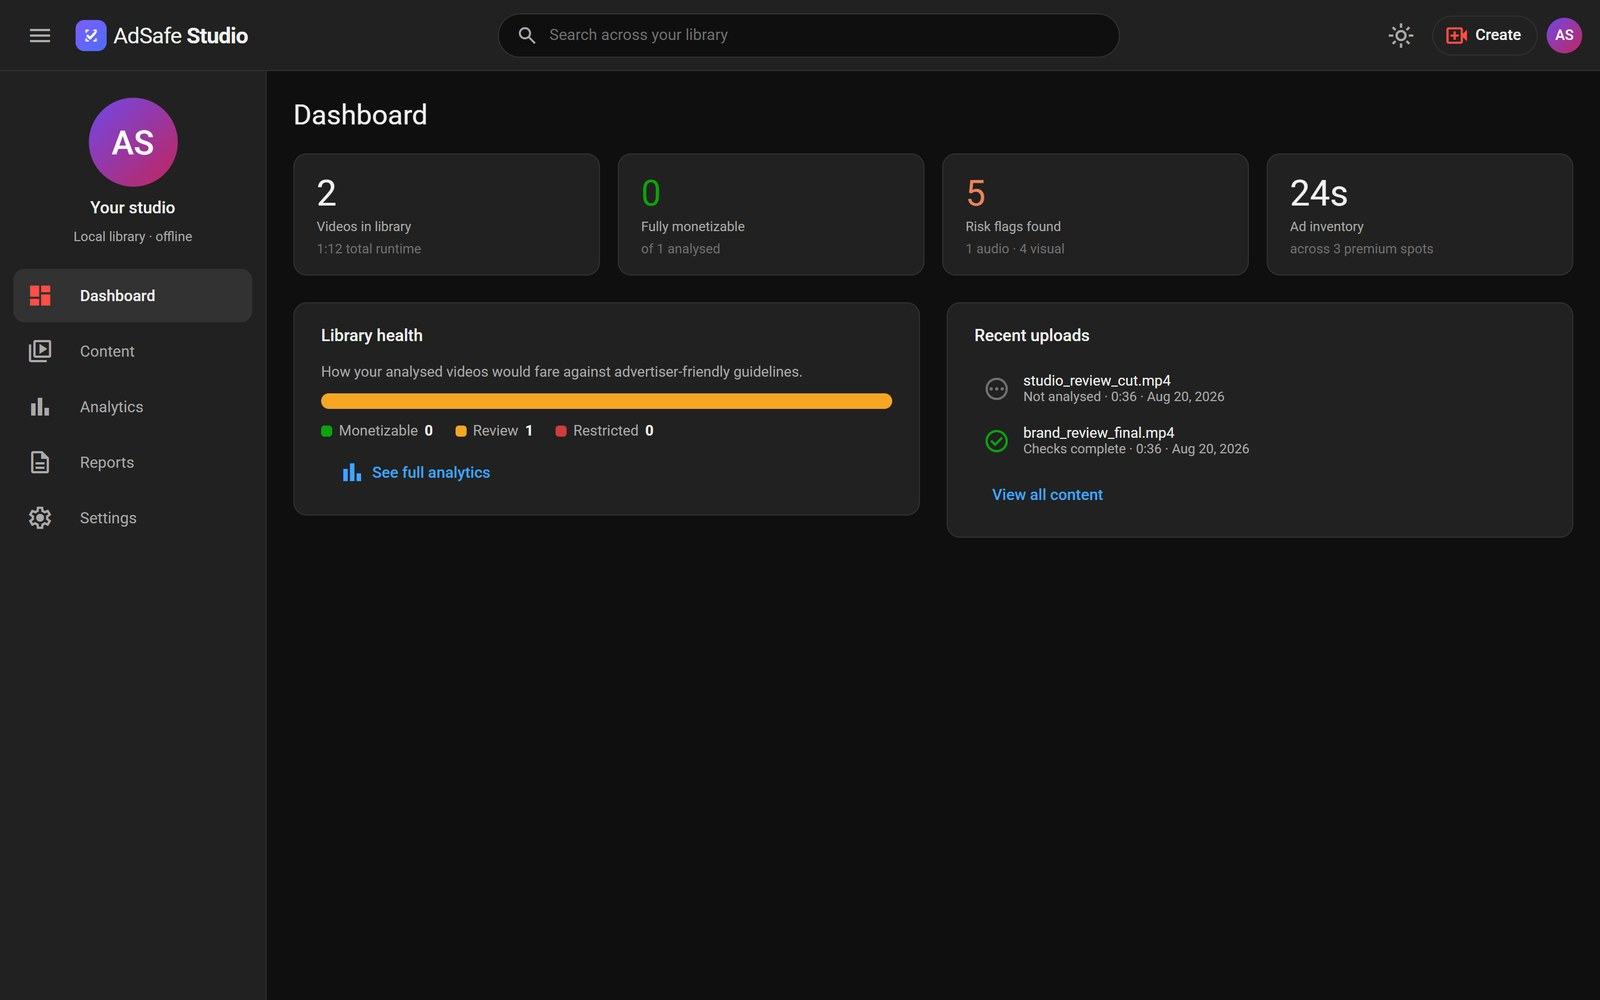
\includegraphics[width=0.95\textwidth]{Images/01-dashboard.jpg}
\caption{Dashboard Screen}
\end{figure}

The dashboard summarises the library: total videos, how many are fully
monetizable, the number of risk flags found, the total advertisement inventory
in seconds, a library-health split bar, and recent uploads with their status.

\subsection{Content Screen}

\begin{figure}[H]
\centering
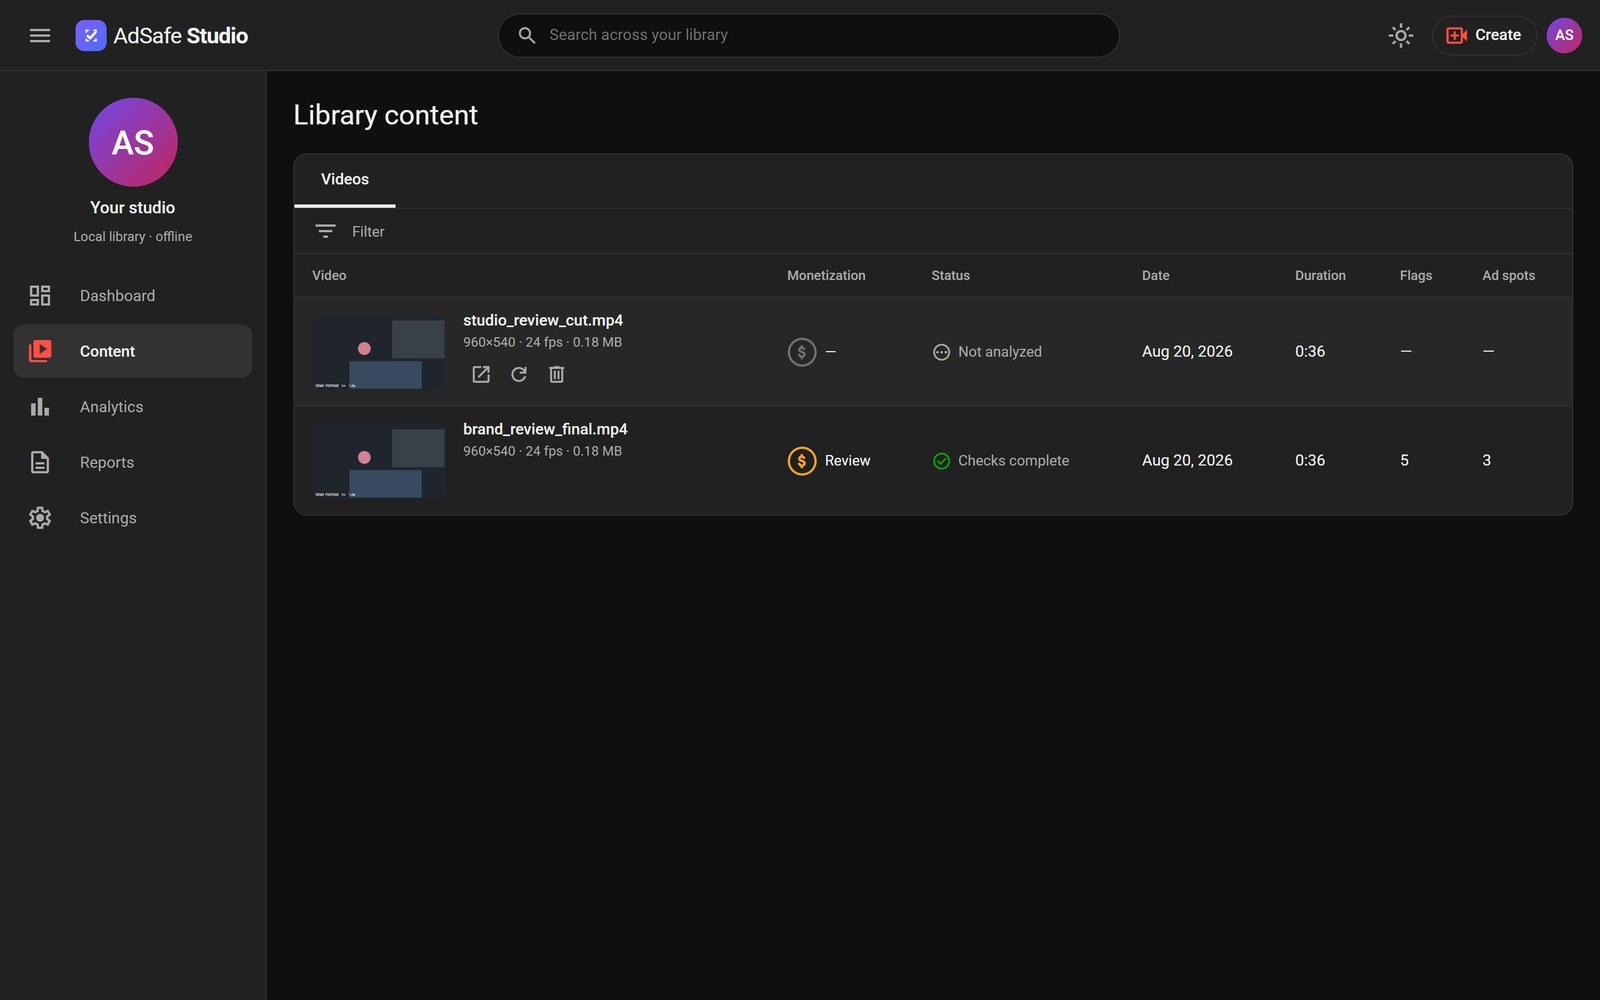
\includegraphics[width=0.95\textwidth]{Images/02-content.jpg}
\caption{Content Screen}
\end{figure}

The content table lists each video with its monetisation verdict, processing
status, duration, flag count and advertisement-spot count. Row actions appear on
hover.

\subsection{Video Detail Screen}

\begin{figure}[H]
\centering
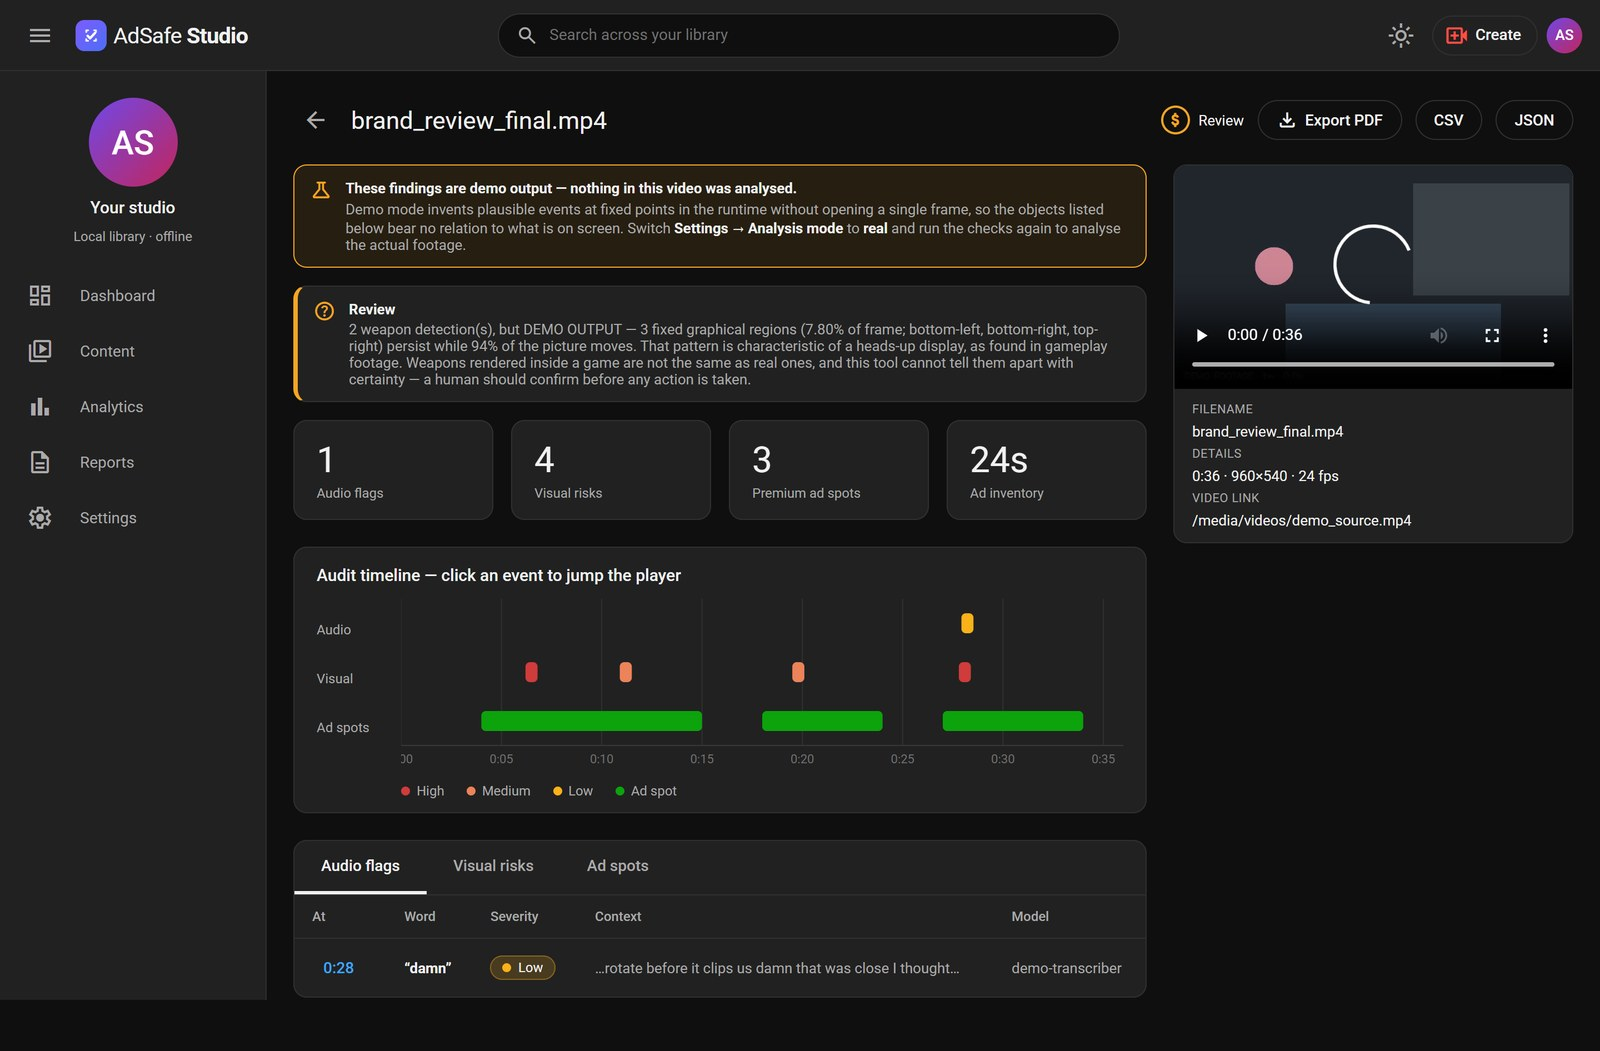
\includegraphics[width=0.95\textwidth]{Images/03-video-detail.jpg}
\caption{Video Detail Screen}
\end{figure}

This is the screen that carries the project's central idea. The verdict appears
with the reasoning that produced it; the audit timeline places every finding
against the runtime and seeks the player when clicked; and each finding records
the engine that produced it in a dedicated column.

\subsection{Responsive Design}

The interface is laid out for four widths: desktop at 1200\,px and above, laptop
from 900 to 1199\,px, tablet from 600 to 899\,px, and mobile below 600\,px. At
tablet width the navigation collapses to a drawer; at mobile width the content
table is re-rendered as a card list, because a seven-column table cannot be made
usable at that width.

\begin{figure}[H]
\centering
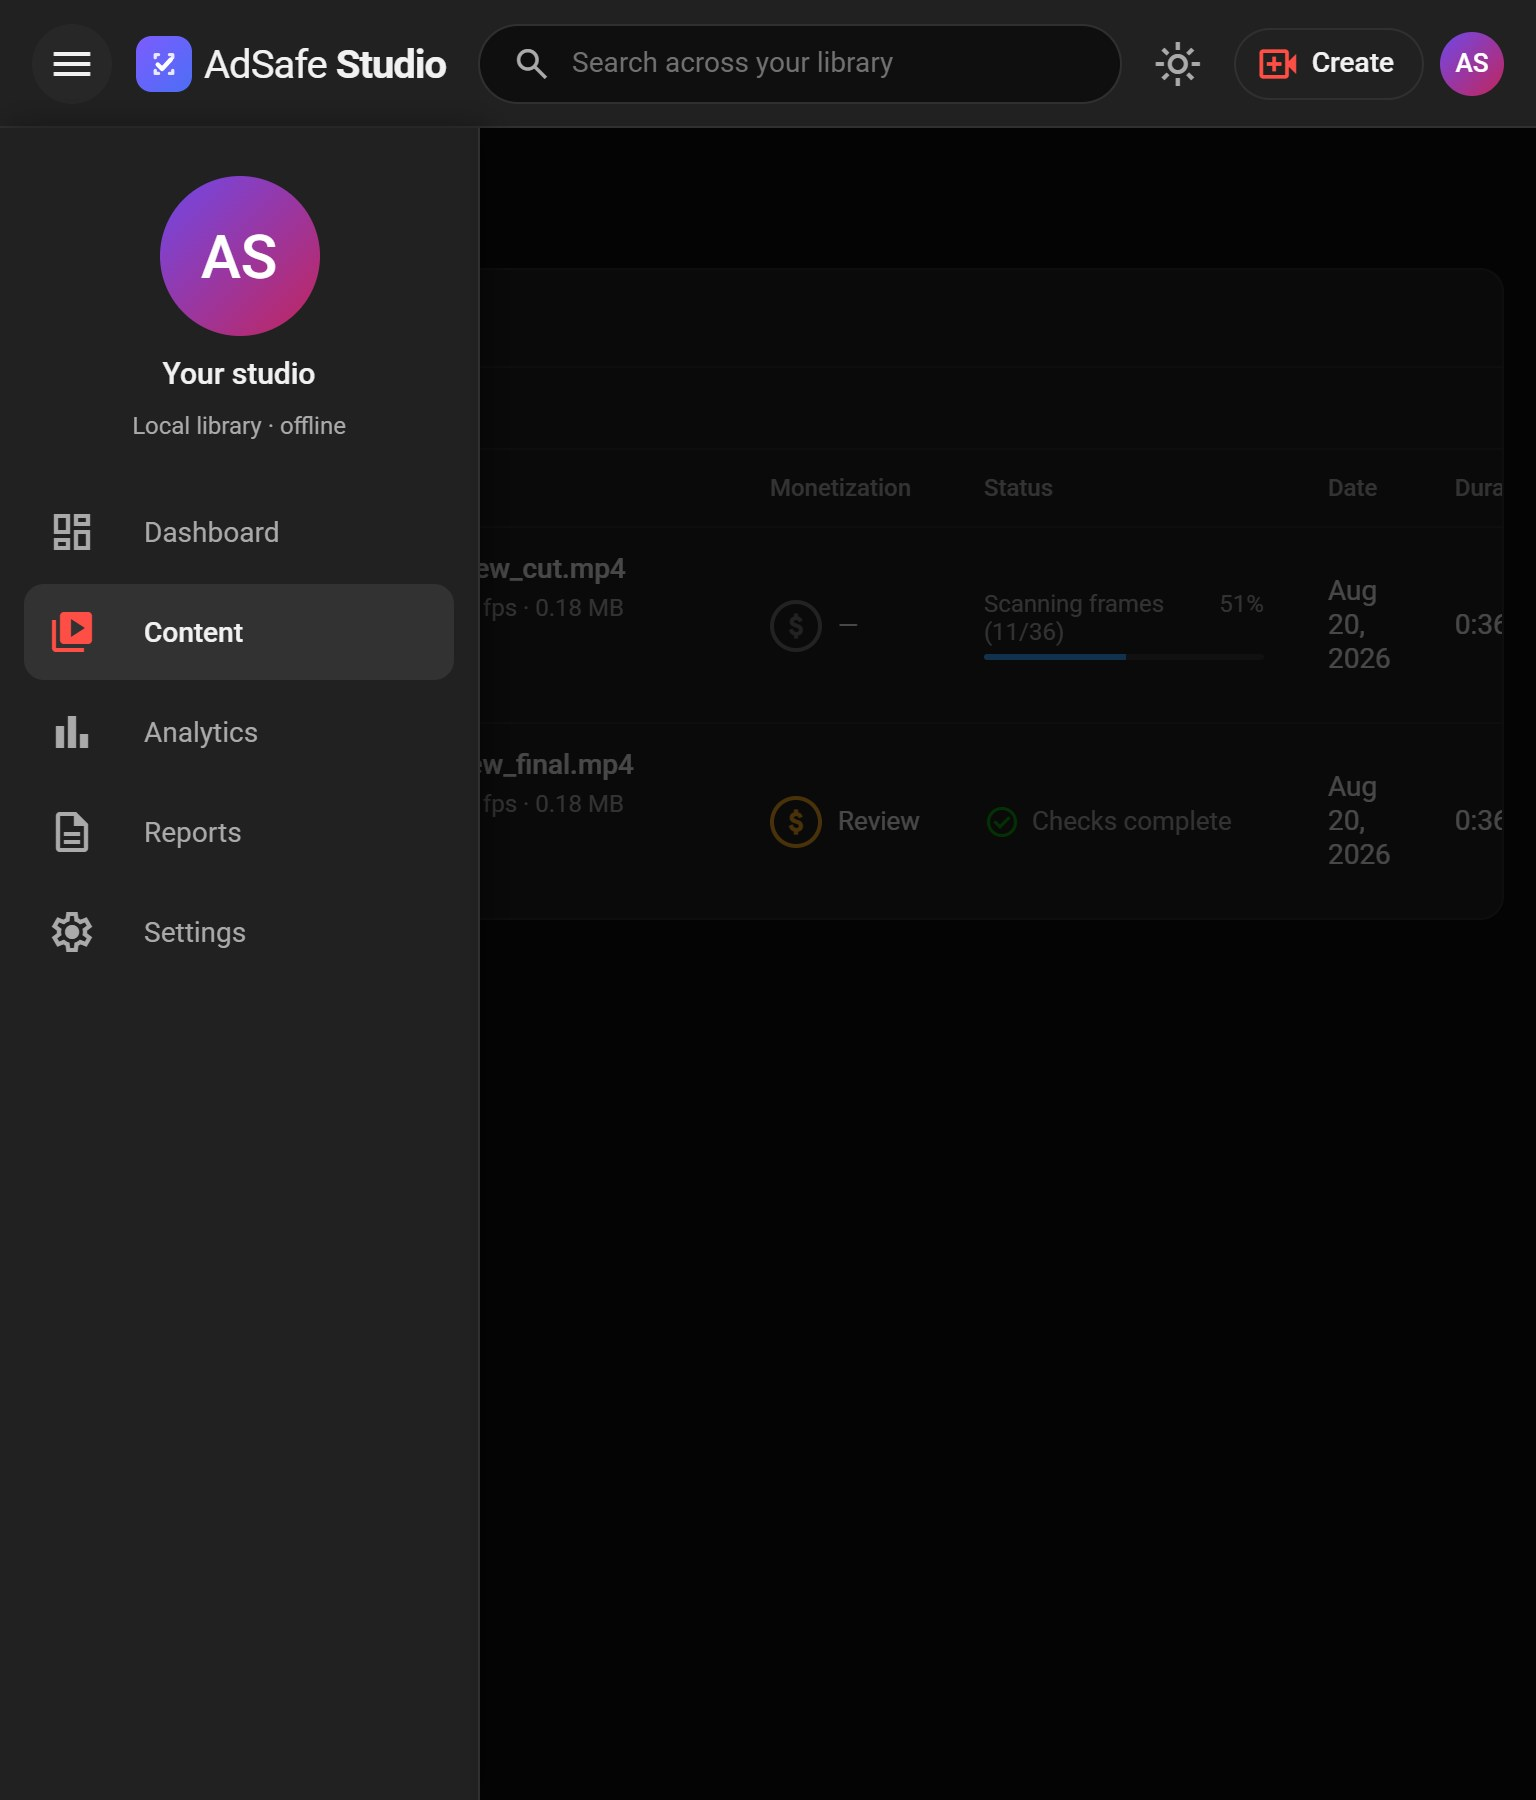
\includegraphics[width=0.42\textwidth]{Images/12-responsive-tablet.jpg}
\hspace{0.4cm}
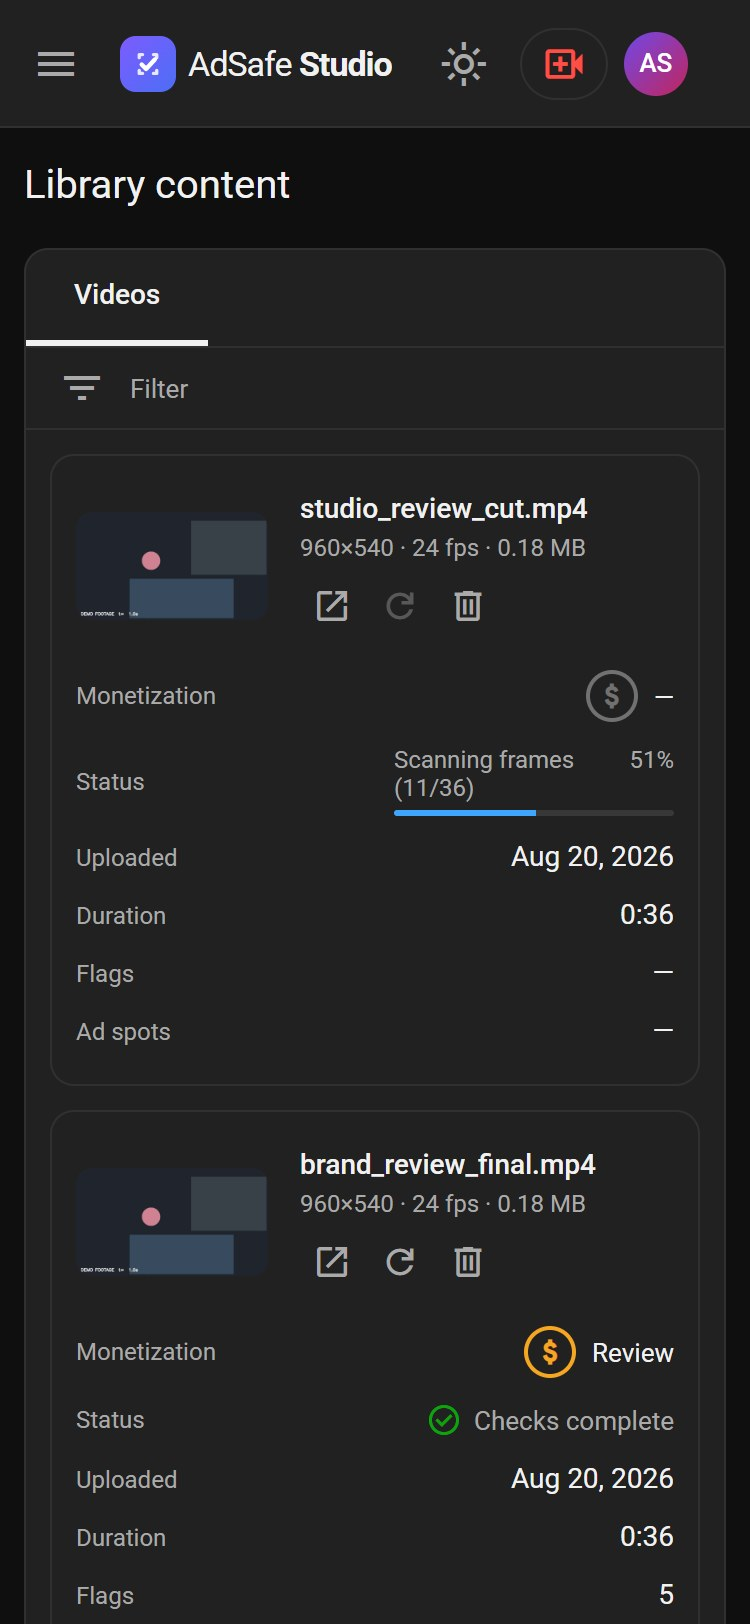
\includegraphics[width=0.24\textwidth]{Images/13-responsive-mobile.jpg}
\caption{Responsive layouts at tablet and mobile widths}
\end{figure}

An automated check verifies that no page scrolls horizontally at any of the
documented widths. It is run before every screenshot capture, and it found three
real layout defects when it was first introduced, described in Chapter~8.

%%%%%%%%%%%%%%%%%%%%%%%%%%%%%%%%%%%%%%%%%%%%%%%%%%
\chapter{Coding and Implementation}
%%%%%%%%%%%%%%%%%%%%%%%%%%%%%%%%%%%%%%%%%%%%%%%%%%

\section{Development Environment}

\begin{table}[H]
\centering
\begin{tabular}{|p{4.5cm}|p{8cm}|}
\hline
\textbf{Component} & \textbf{Selection} \\
\hline
Language and runtime & Python 3.12 \cite{PythonDocs}, Node.js 22,
JavaScript (ES2022) \\
\hline
Backend framework & FastAPI with Uvicorn \cite{FastAPI} \\
\hline
Database & SQLite 3 with write-ahead logging \cite{SQLiteWAL} \\
\hline
Speech recognition & faster-whisper (CTranslate2 backend),
\texttt{base.en} model \\
\hline
Object detection & Ultralytics YOLOv8 \cite{Jocher2023}; COCO weights plus a
project-trained risk model \\
\hline
Image processing & OpenCV, NumPy \cite{OpenCVDocs} \\
\hline
Frontend & React 18, Vite 5, react-router 6, hand-written CSS \\
\hline
Reporting & ReportLab (PDF), pandas (CSV), imageio-ffmpeg \\
\hline
Testing & pytest --- 175 tests \\
\hline
Tooling & Git, matplotlib (diagram generation), Playwright (interface checks) \\
\hline
\end{tabular}
\caption{Development Environment}
\end{table}

\section{Folder Structure}

\begin{lstlisting}[caption={Repository layout}]
specproj/
  backend/            FastAPI application
    main.py           app construction, static and media mounts
    progress.py       in-memory per-video progress state
    routes/           videos.py, system.py  (15 endpoints)
  src/
    audio/            extractor.py, transcriber.py, compliance.py
    vision/           sampler.py, detector.py, overlay.py,
                      adspots.py, tracker.py
    pipeline/         orchestrator.py
    db/               connection.py, repository.py
    reports/          pdf_report.py, exporter.py
    benchmark/        runner.py, evaluator.py
    config.py         paths, supported formats, defaults
  frontend/
    src/pages/        Dashboard, Content, VideoDetail, Analytics,
                      Reports, Settings
    src/components/   Sidebar, TopBar, Timeline, Charts,
                      Badges, UploadDialog
    public/fonts/     Roboto and Material Symbols, served locally
  tests/              12 modules, 175 tests
  benchmark/          clips, labels, intake and evaluation tooling
  training/           fine-tuning pipeline and recorded results
  models/             yolov8n.pt, risk_yolov8.pt
  docs/               diagrams, screenshots, reports, deck
\end{lstlisting}

\section{Module Description}

\subsection{Audio and Language Engine}

The extractor decodes the audio track to a mono WAV file at the sample rate the
recogniser expects. The output path embeds the process identifier, because two
analyses running from separate processes would otherwise collide on a shared
temporary filename. The transcriber runs faster-whisper with
\texttt{word\_timestamps=True}, which is required because the
\texttt{AudioFlags} schema stores per-word start and end times. The compliance
matcher normalises each transcribed word and tests it against the configured
vocabulary.

The vocabulary is built on an explicit severity contract: \textbf{High is
reserved for terms that are unambiguous in isolation}. This matters because a
single High finding is sufficient to restrict a video, so an ambiguous term
placed at High produces false restrictions. An earlier version of the dictionary
did not observe this rule and was rebuilt around it.

\subsection{Vision Engine}

The sampler decodes frames at a configured rate, one frame per second by
default. The detector runs YOLO over each sampled frame and merges the results.

The most consequential implementation detail here is \textbf{multi-scale
inference}. A single resolution cannot serve both a distant object and one
filling the frame: running at 640\,px shrank a real firearm below the resolvable
size and it was missed entirely, while raising the resolution to fix that case
broke a close-up clip that had previously worked. The engine therefore runs each
frame at 640\,px \emph{and} at its native width up to a configurable cap, and
merges the two result sets by intersection over union.

Findings are presented by grouped term. A detection of class \texttt{Handgun},
\texttt{Rifle}, \texttt{Shotgun}, \texttt{Knife}, \texttt{Dagger} or
\texttt{Sword} is reported as \textbf{``Handheld weapon''}, with the model's own
class retained beside it. This is an honesty measure, not a cosmetic one: the
measured per-class results in Chapter~8 show the category is reliable in a way
the specific class is not.

\subsection{The Risk Taxonomy and Why a Model Had to Be Trained}
\label{sec:taxonomy}

The requirements call for the detection of weapons, smoking, alcohol and illicit
substances. Stock YOLOv8 is trained on the COCO 80 classes \cite{Lin2014}, which
contain \textbf{no firearm, no cigarette and no narcotic}. The only adjacent
classes are \texttt{knife}, \texttt{scissors}, \texttt{baseball bat},
\texttt{bottle} and \texttt{wine glass}. A pretrained detector therefore covers
approximately none of the stated taxonomy, and this was confirmed by inspection
before any training was attempted.

The project trained its own detector on a subset of Open Images V7
\cite{Kuznetsova2020}. The available classes were checked against the full Open
Images label set of 601 classes before selection; the shipped model covers ten.

\begin{table}[H]
\centering
\begin{tabular}{|p{3.2cm}|p{3.4cm}|c|c|}
\hline
\textbf{Risk category} & \textbf{Class} & \textbf{Train instances} &
\textbf{mAP@50} \\
\hline
\multirow{6}{*}{Weapon}
 & Knife    & 233  & 0.766 \\
 & Rifle    & 404  & 0.749 \\
 & Handgun  & 84   & 0.487 \\
 & Dagger   & 160  & 0.484 \\
 & Sword    & 123  & 0.420 \\
 & Shotgun  & 169  & 0.339 \\
\hline
\multirow{4}{*}{Substance}
 & Cocktail   & 616  & 0.856 \\
 & Beer       & 365  & 0.723 \\
 & Wine glass & 421  & 0.586 \\
 & Wine       & 1{,}175 & 0.250 \\
\hline
\end{tabular}
\caption{Shipped risk taxonomy and measured per-class performance}
\end{table}

Two consequences follow directly from this table and are reflected in the
system's behaviour.

\textbf{Smoking and narcotics are not detected visually at all}, because Open
Images supplies no usable class for either. They are covered in the audio
vocabulary instead, and the settings screen states this rather than leaving the
user to infer coverage from an absence of findings.

\textbf{Individual weapon classes are unreliable while the category is not.}
\texttt{Shotgun} at 0.339 and \texttt{Sword} at 0.420 are not figures on which
to report a specific object to a user. The category ``weapon'', taken across all
six classes, is considerably more dependable than any one of them. This is
precisely why findings are surfaced as ``Handheld weapon'' with the model's own
class retained beside it, and it is a measurement-driven interface decision
rather than a stylistic one.

\subsection{Overlay Context Engine}
\label{sec:overlay}

This engine answers the question a frame-level detector cannot: is what we are
looking at filmed, or rendered? It accumulates per-pixel temporal statistics in
a streaming pass and identifies regions that stay still while the rest of the
picture moves, and edges that survive in the temporal mean.

The threshold is the part that had to change. An absolute variance gate failed
on real gameplay, because a real heads-up display is translucent and its
contents change --- ammunition counts tick down, health bars move. The gate is
therefore \textbf{relative}: a percentile of the variance distribution within
the frame itself, so a display that is merely much more stable than its
surroundings is detected even when it is not absolutely stable.

\subsection{Advertisement Placement Engine}

Advertisement placement is not an object-detection problem. A blank wall is the
\emph{absence} of objects, and a detector cannot be trained to detect nothing.
The engine builds a binary occupancy matrix per frame from the detected objects
and salient edges, then finds the largest all-clear rectangle within it using a
maximal-rectangle scan. The tracker retains a candidate surface across
consecutive frames and emits it as an advertisement spot only if it persists for
at least five seconds.

\subsection{Orchestration and Verdict}

The orchestrator runs the engines in sequence, reporting progress after each
stage, and finally computes the verdict. The assessment is three-state ---
Monetizable, Review, Restricted --- and returns the reasoning alongside the
label.

\section{Coding Standards}

Python follows PEP 8 with a 88-character soft limit. Modules are organised by
responsibility rather than by type, so that a change to the vision engine
touches one directory. Comments explain \emph{why} rather than \emph{what}, and
in this codebase are used most heavily to record defects that a future change
could silently reintroduce --- for example, the note in the diagram generator
recording that box heights must be computed before layout, and the note in the
stylesheet recording that \texttt{min-width: 0} on a flex item is load-bearing.

JavaScript follows the same principle. Component files are single-purpose, state
is lifted only as far as it needs to go, and the CSS uses a token system with
theme-swapped custom properties rather than hard-coded colours.

\section{Code Efficiency}

Several deliberate efficiency measures were taken.

\textbf{Frames are sampled, not decoded exhaustively.} At one frame per second a
ten-minute video yields 600 frames rather than 15{,}000, which is the difference
between an analysis that finishes during a demonstration and one that does not.

\textbf{Overlay statistics are accumulated in a streaming pass.} Computing
per-pixel variance by retaining every frame would require memory proportional to
the video length; the engine maintains running sums instead, so memory is
constant in the number of frames.

\textbf{Detection resolution is capped and configurable.} The cap is exposed in
the settings screen, with the trade-off stated in the interface itself: raising
it finds smaller objects and costs proportionally more time.

\textbf{The database uses write-ahead logging} \cite{SQLiteWAL}, so that reads
from the interface do not block the single writer performing the analysis.

\section{Parameter Passing}

Engine functions take explicit parameters and return plain data structures
rather than mutating shared state. Configuration is read once at the start of an
analysis and passed down, so a settings change mid-run cannot alter the
behaviour of an analysis already in progress. Progress reporting is passed as a
callback, which keeps the engines free of any dependency on the web layer --- an
engine can therefore be run from a test, or from a script, with no server
present.

\section{Validation Checks}

Validation is applied at three levels.

\textbf{At the boundary.} Uploads are checked against a whitelist of supported
extensions and rejected with a clear message otherwise. The destination filename
is reduced to its final path component before use; the reason is a defect
described in Chapter~\ref{ch:security}.

\textbf{In the application.} The configuration endpoint clamps the detection
resolution into a sensible range rather than rejecting it, because the useful
range is bounded by what the network can resolve at one end and by patience at
the other, and a typo would otherwise make every analysis mysteriously slow or
blind. Analysis mode is restricted to \texttt{demo} or \texttt{real}.

\textbf{In the interface.} The settings screen validates the restricted
vocabulary as it is edited: an empty row or a duplicate term is reported inline
and blocks saving until corrected.

\begin{figure}[H]
\centering
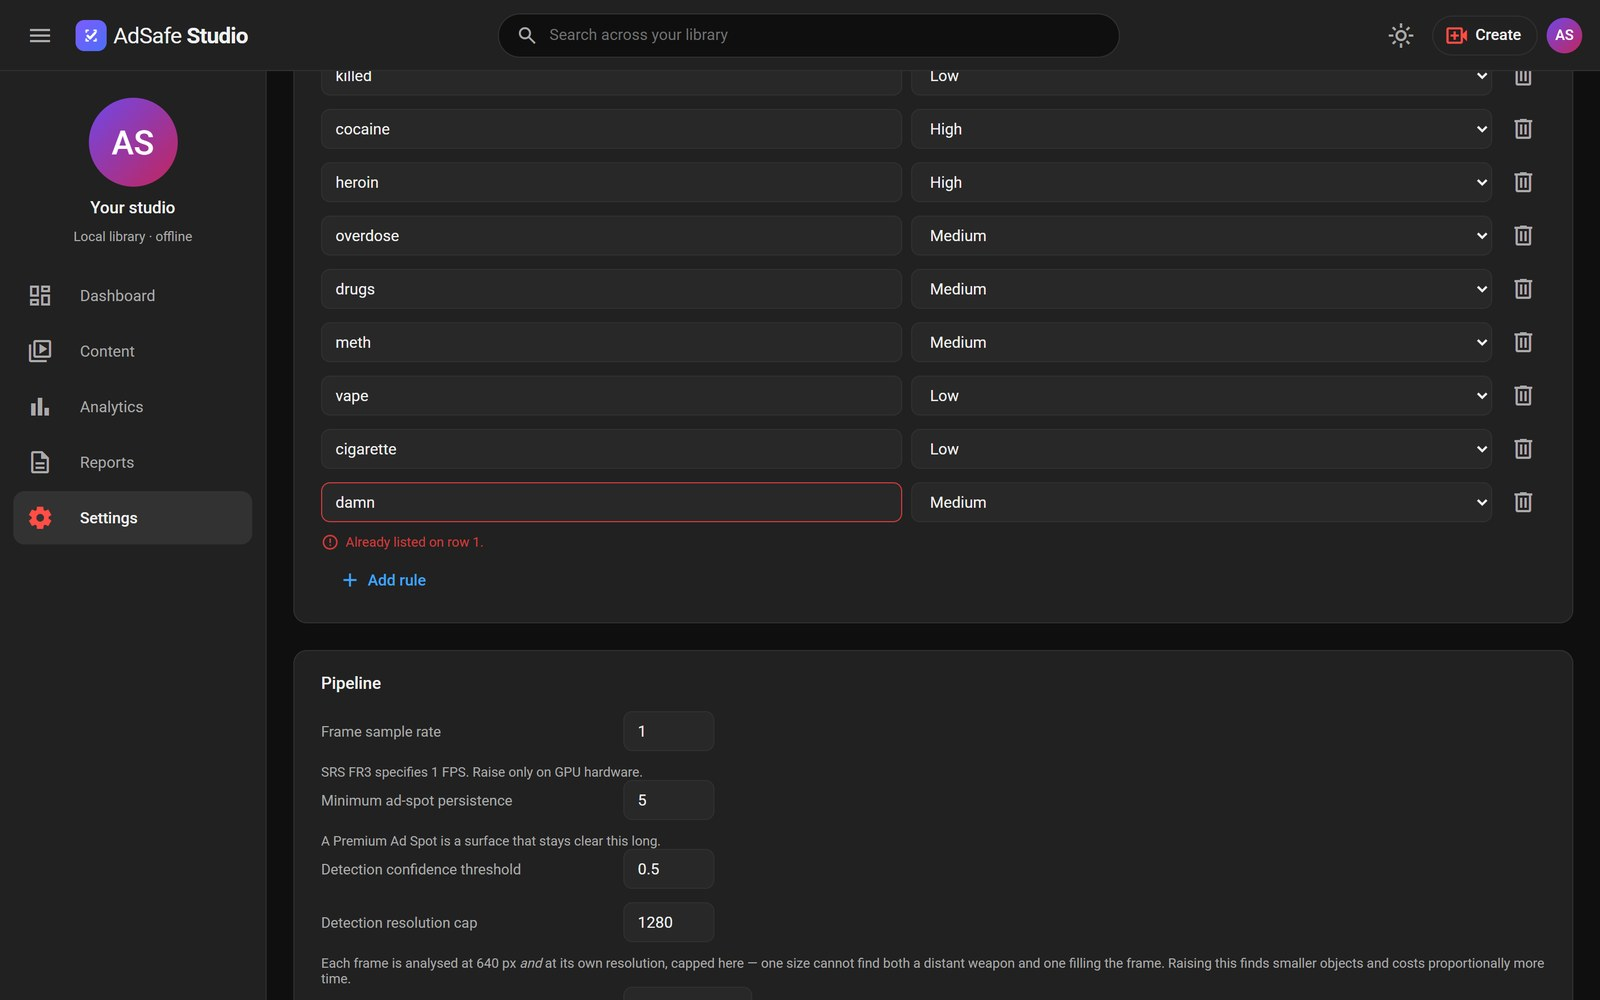
\includegraphics[width=0.95\textwidth]{Images/09-validation.jpg}
\caption{Inline field validation on the settings screen}
\end{figure}

\section{Error Handling}

Unreadable or corrupt media raises a domain error that the API converts into a
400 response with an explanatory message, and the partially written file is
removed. A request to analyse a video already being analysed returns 409 rather
than starting a second run. A request for a video that does not exist returns
404.

Two error-handling decisions are worth recording because they were the result of
failures rather than foresight.

\textbf{The demonstration reset refuses to delete anything if the database is
locked.} It previously deleted files depth-first and then failed partway through
when it reached the locked database, leaving the library in a half-erased state.
It now checks that it can open the database exclusively \emph{before} it removes
anything.

\textbf{The application is smoke-tested at the API level.} A missing import in a
route module once prevented the entire application from starting while all
automated tests passed, because nothing in the suite imported the FastAPI
application. A smoke test that constructs the app now exists precisely to catch
that class of failure.

\section{Important Code Segments}

\begin{lstlisting}[language=Python, caption={Multi-scale inference. One
resolution cannot serve both a distant object and one filling the frame.}]
def inference_scales(frame_width, max_imgsz):
    """640 always; the native width too when it is meaningfully larger."""
    native = min(int(frame_width), int(max_imgsz))
    native = max(MIN_IMGSZ, int(round(native / 32) * 32))
    return (MIN_IMGSZ,) if native <= MIN_IMGSZ else (MIN_IMGSZ, native)


def merge_scale_detections(detections, iou_threshold=0.55):
    """Keep the highest-confidence detection among overlapping duplicates."""
    kept = []
    for det in sorted(detections, key=lambda d: -d["confidence"]):
        if not any(_iou(det["box"], k["box"]) > iou_threshold for k in kept):
            kept.append(det)
    return kept
\end{lstlisting}

\begin{lstlisting}[language=Python, caption={Relative overlay stability. An
absolute gate missed real heads-up displays, which are translucent and change
their contents.}]
def _stability_threshold(self, std):
    # A percentile of the frame's own variance distribution, floored by an
    # absolute value. A HUD only has to be much stiller than its surroundings,
    # not absolutely still.
    return max(float(self.p.stable_std_max),
               float(np.percentile(std, self.p.stable_percentile)))
\end{lstlisting}

\begin{lstlisting}[language=Python, caption={Grouped display labels. The
measured per-class results show the category is reliable where the specific
class is not.}]
WEAPON_CLASSES = {"Handgun", "Rifle", "Shotgun", "Knife", "Dagger", "Sword"}

def display_label(raw_label):
    if raw_label in WEAPON_CLASSES:
        return "Handheld weapon"
    ...
\end{lstlisting}

%%%%%%%%%%%%%%%%%%%%%%%%%%%%%%%%%%%%%%%%%%%%%%%%%%
\chapter{Testing}
%%%%%%%%%%%%%%%%%%%%%%%%%%%%%%%%%%%%%%%%%%%%%%%%%%

\section{Testing Objectives}

Testing had three objectives: to confirm that each component behaves as
specified in isolation; to confirm that the assembled pipeline produces correct
results end to end; and --- the objective that mattered most in practice --- to
determine whether the system behaves correctly on \emph{real} video rather than
on synthetic or held-out data.

The third objective is separated deliberately, because this project produced
direct evidence that the first two are not sufficient.

\section{Testing Techniques Used}

\begin{itemize}[itemsep=3pt]
\item \textbf{Unit testing} of pure functions: the maximal-rectangle search, the
IoU merge, severity assignment, verdict computation and label mapping.
\item \textbf{Integration testing} of the repository against a temporary
database, including cascade behaviour and migrations.
\item \textbf{API smoke testing}, which constructs the FastAPI application and
exercises the endpoints.
\item \textbf{Security testing} of the upload path against directory traversal.
\item \textbf{Automated interface testing} with a headless browser, covering
layout overflow at five widths across six pages, and offline rendering.
\item \textbf{Manual evaluation on real video}, which is where the significant
defects were found.
\end{itemize}

\section{Testing Strategy}

Unit tests run against every commit and must all pass. Interface checks run
before every screenshot capture, so that a layout regression cannot silently
reach the documentation. Model changes are gated on real-video behaviour and not
on validation metrics --- a rule adopted after the evidence in
Section~\ref{sec:runtwo}.

\section{Testing Plan}

\begin{table}[H]
\centering
\begin{tabular}{|p{4.6cm}|c|p{6cm}|}
\hline
\textbf{Area} & \textbf{Tests} & \textbf{Focus} \\
\hline
Vision engine & 36 & Scale selection, merging, label mapping, coverage \\
\hline
Advertisement spots & 27 & Maximal rectangle, scoring, edge cases \\
\hline
Benchmark harness & 18 & Scoring, gating, refusal to publish \\
\hline
Overlay detection & 16 & Stability thresholds, region reporting \\
\hline
Reports & 13 & PDF, CSV and JSON export \\
\hline
Repository & 12 & CRUD, cascade delete, migrations \\
\hline
Verdict determination & 12 & Three-state logic and reasoning text \\
\hline
Audio engine & 7 & Extraction, matching, severity \\
\hline
API smoke & 7 & Application construction and endpoints \\
\hline
Upload security & 6 & Directory traversal, extension whitelist \\
\hline
Spot tracker & 5 & Persistence across frames \\
\hline
Compliance & 4 & Aggregation \\
\hline
\textbf{Total} & \textbf{175} & \\
\hline
\end{tabular}
\caption{Test Distribution by Area}
\end{table}

\section{Unit Test Cases}

\begin{table}[H]
\centering
\small
\begin{tabular}{|c|p{3cm}|p{3.4cm}|p{3.4cm}|c|}
\hline
\textbf{TC ID} & \textbf{Input} & \textbf{Expected Output} &
\textbf{Actual Output} & \textbf{Status} \\
\hline
TC01 & Frame width 1920, cap 1280 & Scales (640, 1280) & (640, 1280) & Pass \\
\hline
TC02 & Frame width 640, cap 1280 & Single scale (640,) & (640,) & Pass \\
\hline
TC03 & Two boxes, IoU 0.8 & Higher confidence kept, one result & One result &
Pass \\
\hline
TC04 & Occupancy matrix, clear 40\% region & Largest rectangle returned &
Correct rectangle & Pass \\
\hline
TC05 & Surface present 3\,s & Not emitted (below 5\,s) & Not emitted & Pass \\
\hline
TC06 & Surface present 7\,s & Emitted as ad spot & Emitted & Pass \\
\hline
TC07 & Class ``Handgun'' & Display label ``Handheld weapon'' & ``Handheld
weapon'' & Pass \\
\hline
TC08 & One High-severity term & Verdict Restricted & Restricted & Pass \\
\hline
TC09 & Weapon plus overlay evidence & Verdict Review, reasoning cites overlay &
Review with reasoning & Pass \\
\hline
TC10 & Delete parent video & All child rows cascade & All removed & Pass \\
\hline
\end{tabular}
\caption{Unit Test Cases}
\end{table}

\section{System Test Cases}

\begin{table}[H]
\centering
\small
\begin{tabular}{|c|p{3cm}|p{3.4cm}|p{3.4cm}|c|}
\hline
\textbf{TC ID} & \textbf{Input} & \textbf{Expected Output} &
\textbf{Actual Output} & \textbf{Status} \\
\hline
ST01 & Upload valid MP4 & 201, metadata stored, thumbnail generated & As
expected & Pass \\
\hline
ST02 & Upload \texttt{.exe} & 400, format rejected & 400 with message & Pass \\
\hline
ST03 & Upload named \texttt{a/../../../../evil.mp4} & Stored inside the video
directory & Stored safely & Pass \\
\hline
ST04 & Analyse a video & Findings written, verdict computed, status completed &
As expected & Pass \\
\hline
ST05 & Analyse an already-running video & 409 conflict & 409 & Pass \\
\hline
ST06 & Poll status mid-analysis & Stage and percentage reported & ``Scanning
frames (1/36)'', 41\% & Pass \\
\hline
ST07 & Export PDF, CSV, JSON & Three files written and downloadable & As
expected & Pass \\
\hline
ST08 & Load all six pages at five widths & No horizontal overflow & 30/30 clean
& Pass \\
\hline
ST09 & Load interface with all external traffic blocked & All icons render &
118/118 rendered & Pass \\
\hline
\end{tabular}
\caption{System Test Cases}
\end{table}

\section{Test Reports}

\subsection{Automated Suite}

The suite reports \textbf{175 passed} with no failures.

\subsection{Results on Real Video}

Four real clips were analysed during development. \textbf{Each one exposed a
defect that synthetic testing had not.} This is the single most useful result in
the project's testing history and is reported in full.

\begin{table}[H]
\centering
\small
\begin{tabular}{|p{3.4cm}|p{4.4cm}|p{5cm}|}
\hline
\textbf{Clip} & \textbf{Observed failure} & \textbf{Change made} \\
\hline
News footage, firearm at a distance & Firearm not detected at all & Multi-scale
inference: 640\,px alone shrank it below the resolvable size \\
\hline
Firearm in close-up & Detected, but raising resolution to fix the previous case
broke this one & Merge results from both scales rather than choosing one \\
\hline
Counter-Strike gameplay & Heads-up display not detected as an overlay &
Percentile-based stability threshold instead of an absolute one \\
\hline
Demonstration-mode run on a real clip & Invented findings indistinguishable from
measured ones & Per-finding engine provenance recorded and displayed \\
\hline
\end{tabular}
\caption{Defects found only by testing on real video}
\end{table}

\subsection{Model Evaluation}
\label{sec:runtwo}

Two fine-tuning runs were performed. Run~1 is the shipped model.

\begin{table}[H]
\centering
\begin{tabular}{|p{4cm}|c|c|}
\hline
\textbf{Metric} & \textbf{Run 1 (shipped)} & \textbf{Run 2 (rejected)} \\
\hline
Precision & 0.569 & higher \\
\hline
Recall & 0.548 & higher \\
\hline
mAP@50 & 0.566 & \textbf{0.591} \\
\hline
mAP@50--95 & \textbf{0.432} & 0.396 \\
\hline
Handgun mAP@50 & 0.487 & \textbf{0.546} \\
\hline
\textbf{Detections of a real firearm} & \textbf{13} & \textbf{0} \\
\hline
\end{tabular}
\caption{Fine-tuning run comparison}
\end{table}

\textbf{Run~2 improved almost every headline metric and was rejected.} On the
test clip containing a real pistol, run~1 produced thirteen detections and run~2
produced none. A validation set drawn from the training distribution did not
predict behaviour on video --- and this was demonstrated twice, since run~1 had
itself scored only 0.487 on Handgun and still detected the weapon that run~2
missed entirely.

The per-class results carry a second finding worth recording. \texttt{Wine} had
the most training data of any class, 1{,}175 instances, and scored the worst at
0.250. \texttt{Handgun} had the least, 84 instances, and scored 0.487. More data
did not mean better performance; at the extremes the relationship was inverted.
The cause is class definition rather than volume: in the source dataset ``Wine''
is applied to bottles, to filled glasses and to the liquid itself, overlapping
two other classes, so the model cannot draw a boundary that the labels do not.

\subsection{Accuracy on Creator Footage}
\label{sec:accuracy}

\textbf{No precision or recall figure is claimed on real creator footage.}

The benchmark harness required to establish one is implemented, along with clip
intake and a labelling interface. Its coverage gates require at least ten real
clips, at least thirty labelled events and some clean clips to detect false
positives. \textbf{At the time of writing, zero of the twenty planned clips have
been labelled}, so none of these gates is met, and the harness refuses by design
to publish a figure from insufficient evidence.

This is stated plainly rather than omitted. An earlier requirements document
asserted a precision above 85\%; that figure was never measured and is withdrawn
here. Completing the labelled corpus is the first item of future work in
Chapter~12.

\subsection{Offline Verification}
\label{sec:offlinecheck}

An automated check aborts every network request that is not to localhost and
then loads all six pages. It reports \textbf{zero external requests attempted}
and confirms that all 118 icon elements render as glyphs.

The check was written because the interface previously loaded its fonts from a
content delivery network while the product claimed to run entirely offline. With
no network, every icon fell back to its own ligature name, the navigation read
as plain text and the application appeared broken. The fonts are now served by
the application itself.

The check is also verified to be capable of failing: with the local font
deliberately blocked, it correctly reports all twenty icons on the content page
as text.

\section{Debugging and Code Improvement}

Several defects were found and fixed during the final testing phase. Three are
recorded here because each was invisible to the automated suite and was found
only by attempting to automate something else.

\textbf{The progress bar usually never appeared.} The analyse endpoint returns
202 as soon as the job is queued, before the background task writes the
processing status. The interface refetched immediately, won the race, received
``pending'', and therefore never started the poll that drives the progress bar.
In demonstration mode this is invisible because an analysis completes in about
two tenths of a second; in real mode the interface appears to do nothing for the
whole run. The interface now marks the row as processing from the response it
already received.

\textbf{The video detail page scrolled sideways at 1440\,px.} A flex item
defaults to \texttt{min-width: auto} and so refuses to shrink below its content;
the findings table pushed the main column 150\,px past its container. The same
cause applied one level down, where a bare \texttt{1fr} grid track floors at
min-content.

\textbf{The content table had no scroll container}, so it widened the page at
1024 and 768\,px. Correcting that revealed that the mobile card rows were
\texttt{width: 100\%} plus 12\,px side margins --- 24\,px wider than the space
available --- which had been clipping the right edge of every card.

After these fixes, all thirty page-and-width combinations are clean.

%%%%%%%%%%%%%%%%%%%%%%%%%%%%%%%%%%%%%%%%%%%%%%%%%%
\chapter{System Security Measures}
\label{ch:security}
%%%%%%%%%%%%%%%%%%%%%%%%%%%%%%%%%%%%%%%%%%%%%%%%%%

\section{Introduction}

Security for this system must be assessed against what it actually is: a
single-user desktop application that runs on the creator's own machine, binds to
localhost, and is not exposed to a network. Applying a multi-user web threat
model to it would produce a chapter describing controls that do not exist and
would misrepresent the system.

This chapter therefore states the threat model plainly, describes the controls
that are implemented, and identifies explicitly what is \emph{not} protected and
why.

\section{Threat Model}

\textbf{Assets.} Unpublished video files, the findings derived from them, and
the local database.

\textbf{Trusted.} The machine, its operating-system user account and its
filesystem permissions.

\textbf{In scope.} Malformed or hostile input reaching the API --- a crafted
upload, an out-of-range configuration value, a malicious filename. Accidental
data loss. Unintended transmission of user content off the machine.

\textbf{Out of scope.} An attacker with an interactive session on the machine
already has the video files; the application cannot defend against that. Network
attackers are out of scope because the application binds to localhost and makes
no outbound connections.

\section{Authentication Mechanism}

\textbf{The system implements no authentication, and this is a deliberate scope
decision rather than an omission.} The application is single-user and local;
there are no accounts, and the operating system's own login is the authentication
boundary. Adding a password to a locally bound single-user tool would add an
obstacle without adding protection, since anyone able to reach the port already
has the user's session and can read the video files directly.

The consequence is stated honestly: \textbf{if the server were bound to a
public interface, it would be completely unprotected.} It binds to localhost,
and Section~\ref{sec:netsec} states what would be required before that could
safely change.

\section{Authorization Mechanism}

There is a single implicit role --- the local user --- with full access to every
function. No role-based access control is implemented, for the same reason as
above. Were the system extended to multiple users, the roles below would be the
minimum required; they are documented as design intent, not as implemented
functionality.

\begin{table}[H]
\centering
\begin{tabular}{|p{3cm}|p{4.5cm}|p{4.5cm}|}
\hline
\textbf{Role} & \textbf{Would be permitted} & \textbf{Would be denied} \\
\hline
Creator & Upload, analyse, read own findings, export & Access to other users'
videos; configuration changes \\
\hline
Reviewer & Read findings, export & Upload, delete, configuration changes \\
\hline
Administrator & All of the above, plus vocabulary and pipeline configuration &
--- \\
\hline
\end{tabular}
\caption{Role-Based Access Control (design intent, not implemented)}
\end{table}

\section{User Profiles and Access Rights}

The application stores no user profile of any kind: no name, no email address,
no credentials, no telemetry identifier. The only persisted state is the video
library, the findings derived from it, and the pipeline configuration. This is a
direct consequence of the local single-user model and is one of the system's
stronger privacy properties.

\section{Database Security}

\textbf{Injection.} All query parameters are bound rather than interpolated. One
statement in the data layer composes SQL with an f-string, and it interpolates a
fixed module-level constant --- never a request value --- so no user input can
reach the query text \cite{OWASPTop10}.

\textbf{Referential integrity.} \texttt{PRAGMA foreign\_keys = ON} is issued on
every connection, and all child relationships are \texttt{ON DELETE CASCADE}, so
deleting a video cannot leave orphaned findings.

\textbf{Constraint enforcement.} Check constraints on status, severity, risk
category and report type mean an invalid value cannot be written by any code
path, including a future one.

\textbf{Concurrency.} Write-ahead logging is enabled and there is exactly one
writer, so an interrupted analysis cannot corrupt the database
\cite{SQLiteWAL}.

\section{Data Security}

\textbf{Uploads are restricted by extension} to MP4, MOV and AVI, checked
against a whitelist rather than a blacklist.

\textbf{Directory traversal in the upload path was found and fixed during this
phase, and is reported here rather than quietly corrected.} The handler
interpolated the client-supplied filename directly into the destination path. A
crafted multipart request with the filename
\texttt{a/../../../../evil.mp4} normalised to a location outside the repository
entirely, and the extension check did not catch it because only the final path
component is inspected --- the suffix was still \texttt{.mp4}. Ordinary browsers
do not send path components, but the endpoint is reachable directly by any HTTP
client. The handler now reduces the supplied name to its final component before
using it, and six regression tests cover the traversal patterns. Those tests were
themselves verified against the vulnerable code to confirm they fail when the
defect is present.

\textbf{Deletion is complete.} Removing a video deletes the stored file, its
thumbnail, its progress state and, by cascade, every finding derived from it.

\textbf{A known gap: uploads are not size-limited.} A very large file can
exhaust local disk. For a single-user local tool the impact is limited to the
user's own machine, so this is recorded as a limitation rather than treated as a
vulnerability, and it is listed in Chapter~12.

\section{Network Security}
\label{sec:netsec}

The application binds to localhost and is not exposed to a network. More
significantly, \textbf{it makes no outbound connection either}. This is verified
automatically rather than asserted: the offline check described in
Section~\ref{sec:offlinecheck} severs every non-localhost request and confirms
the interface still functions, reporting zero external requests attempted.

This property was not free. The interface previously loaded fonts from a content
delivery network, which both broke the offline claim and left the application
looking broken on a machine without internet access. Both fonts are now served
by the application itself.

Before the server could safely be bound to a non-local interface, the following
would be required: authentication and session management; transport encryption;
per-user authorisation on every endpoint; upload size limits and rate limiting;
and a cross-origin policy. None of these is implemented, and the system should
not be exposed to a network until they are.

\section{Security Best Practices}

\begin{itemize}[itemsep=3pt]
\item Input validated at the boundary against whitelists.
\item Parameterised queries throughout.
\item Constraints enforced by the database, not only by application code.
\item Least privilege by construction: no accounts, no credentials, no stored
personal data.
\item No outbound network access, verified by an automated check.
\item Dependencies pinned in \texttt{requirements.txt}, following an incident in
which an unpinned NumPy 2 upgrade broke binary compatibility with two packages
at startup.
\item Security defects documented rather than silently patched, so that the
reasoning survives.
\end{itemize}

\section{Licensing}
\label{sec:licensing}

Ultralytics YOLOv8 is distributed under AGPL-3.0 \cite{Jocher2023}. This is
recorded explicitly because the licence extends to models trained with the
software, not merely to the source code, and therefore covers the fine-tuned
weights produced by this project. The project is academic and non-distributed,
which is compatible with those terms; any future distribution would need to
comply with AGPL-3.0 or obtain a commercial licence.

%%%%%%%%%%%%%%%%%%%%%%%%%%%%%%%%%%%%%%%%%%%%%%%%%%
\chapter{Cost Estimation}
%%%%%%%%%%%%%%%%%%%%%%%%%%%%%%%%%%%%%%%%%%%%%%%%%%

\section{Introduction}

Cost estimation determines the resources required to complete a project
\cite{Boehm1981}. Two figures are given here and should not be confused. The
\textbf{actual cost incurred} is what the project really spent, which for an
academic project using open-source software on existing hardware is
approximately zero. The \textbf{notional cost} is what the same work would cost
if commissioned commercially, derived below using COCOMO; it is an academic
exercise, not money spent.

\section{Development Cost}

\begin{table}[H]
\centering
\begin{tabular}{|p{6cm}|p{2.6cm}|p{3.4cm}|}
\hline
\textbf{Item} & \textbf{Actual (INR)} & \textbf{Notional (INR)} \\
\hline
Development effort & 0 & 8{,}68{,}000 \\
\hline
Testing effort & 0 & 1{,}45{,}000 \\
\hline
Documentation effort & 0 & 87{,}000 \\
\hline
\textbf{Total} & \textbf{0} & \textbf{11{,}00{,}000} \\
\hline
\end{tabular}
\caption{Development Cost Estimation}
\end{table}

Actual cost is zero because the work was performed by the project team as part
of the academic programme. The notional column applies the COCOMO effort of
Section~\ref{sec:cocomo} at an indicative rate of INR 50{,}000 per
person-month.

\section{Hardware Cost}

\begin{table}[H]
\centering
\begin{tabular}{|p{6cm}|p{2.6cm}|p{3.4cm}|}
\hline
\textbf{Hardware Component} & \textbf{Actual (INR)} & \textbf{Note} \\
\hline
Development laptops (4, already owned) & 0 & Intel Core i5 class, 8--16\,GB RAM
\\
\hline
Storage (approx. 5\,GB) & 0 & Existing local storage \\
\hline
GPU for model training & 0 & Google Colab free tier, one T4 session \\
\hline
Networking equipment & 0 & Not required; the system runs offline \\
\hline
\textbf{Total} & \textbf{0} & \\
\hline
\end{tabular}
\caption{Hardware Cost}
\end{table}

The zero in the networking row is a genuine architectural consequence rather
than an accounting convenience: the system performs no network communication, so
no server, bandwidth or hosting cost arises at any point in its lifetime.

\section{Software Cost}

\begin{table}[H]
\centering
\begin{tabular}{|p{5cm}|p{2.4cm}|p{4.6cm}|}
\hline
\textbf{Software} & \textbf{Cost (INR)} & \textbf{Licence} \\
\hline
Python 3.12 & 0 & PSF \\
\hline
FastAPI, Uvicorn & 0 & MIT \\
\hline
SQLite 3 & 0 & Public domain \\
\hline
React, Vite & 0 & MIT \\
\hline
faster-whisper, CTranslate2 & 0 & MIT \\
\hline
Ultralytics YOLOv8 & 0 & \textbf{AGPL-3.0} (see
Section~\ref{sec:licensing}) \\
\hline
OpenCV, NumPy, pandas, ReportLab & 0 & BSD / Apache / BSD \\
\hline
Open Images V7 subset & 0 & CC BY 4.0 \\
\hline
\textbf{Total} & \textbf{0} & \\
\hline
\end{tabular}
\caption{Software Cost}
\end{table}

\section{Maintenance Cost}

Maintenance for a locally installed tool with no server component is limited to
dependency updates, model refreshes and defect correction. Estimated at 15\% of
notional development effort per year, this is approximately INR 1{,}65{,}000
annually in notional terms, or roughly 3.3 person-months. The absence of hosting
means there is no recurring infrastructure cost at all --- the dominant ongoing
expense for a comparable cloud service.

\section{Cost Estimation Model}

Basic COCOMO is used \cite{Boehm1981}. The project is classified as
\textbf{organic}: a small team, working in a familiar problem domain, with
requirements that were flexible rather than externally fixed. Intermediate
COCOMO was not applied because reliable cost-driver ratings are not available
for a student project of this size, and applying them would give the estimate a
false appearance of precision.

\section{COCOMO Estimation}
\label{sec:cocomo}

\subsection{Formula}

\[
E = a(\mathrm{KLOC})^{b}
\qquad
D = c(E)^{d}
\]

For organic projects $a = 2.4$, $b = 1.05$, $c = 2.5$ and $d = 0.38$.

\subsection{Size}

\begin{table}[H]
\centering
\begin{tabular}{|p{6cm}|c|}
\hline
\textbf{Component} & \textbf{Lines of code} \\
\hline
Python (backend, engines, data layer) & 3{,}683 \\
\hline
JavaScript, JSX and CSS (interface) & 2{,}437 \\
\hline
\textbf{Delivered source subtotal} & \textbf{6{,}120} \\
\hline
Automated tests (excluded from KLOC) & 1{,}754 \\
\hline
\end{tabular}
\caption{Source size}
\end{table}

Test code is excluded from the size input, since COCOMO's coefficients already
account for testing effort; including it would double-count.

\subsection{Calculation}

With $\mathrm{KLOC} = 6.120$:

\[
E = 2.4 \times (6.120)^{1.05} \approx 2.4 \times 6.79 \approx
\mathbf{16.3\ \text{person-months}}
\]

\[
D = 2.5 \times (16.3)^{0.38} \approx 2.5 \times 2.86 \approx
\mathbf{7.2\ \text{months}}
\]

\[
\text{Average staffing} = E / D \approx 16.3 / 7.2 \approx
\mathbf{2.3\ \text{persons}}
\]

\subsection{Comparison with Actual Effort}

The model estimates 16.3 person-months over 7.2 months with 2.3 staff. The
project was delivered by four people over roughly 14 weeks, which is
approximately 3.2 calendar months and therefore substantially faster than the
model predicts.

The discrepancy is worth stating rather than hiding. Three factors account for
it. First, a large proportion of the functionality is supplied by mature
libraries; the delivered line count reflects integration and orchestration
rather than algorithms written from first principles. Second, COCOMO's organic
coefficients were calibrated on projects with far more requirements
formalisation and process overhead than an academic project carries. Third, and
most significantly, AI assistance was used throughout development, as disclosed
in the project's AI usage declaration; COCOMO predates such tooling entirely and
cannot account for it. The estimate should therefore be read as an academic
exercise in applying the model, not as a claim about how long this work would
have taken under the conditions COCOMO assumes.

\section{Cost Summary}

\begin{table}[H]
\centering
\begin{tabular}{|p{6cm}|p{2.8cm}|p{3.2cm}|}
\hline
\textbf{Category} & \textbf{Actual (INR)} & \textbf{Notional (INR)} \\
\hline
Development, testing, documentation & 0 & 11{,}00{,}000 \\
\hline
Hardware & 0 & 0 \\
\hline
Software licences & 0 & 0 \\
\hline
Infrastructure and hosting & 0 & 0 \\
\hline
\textbf{Total} & \textbf{0} & \textbf{11{,}00{,}000} \\
\hline
\end{tabular}
\caption{Cost Summary}
\end{table}

%%%%%%%%%%%%%%%%%%%%%%%%%%%%%%%%%%%%%%%%%%%%%%%%%%
\chapter{Reports and Outputs}
%%%%%%%%%%%%%%%%%%%%%%%%%%%%%%%%%%%%%%%%%%%%%%%%%%

\section{Introduction}

This chapter presents the reports the system generates and the screens through
which its outputs are read.

\section{Dashboard Report}

\begin{figure}[H]
\centering
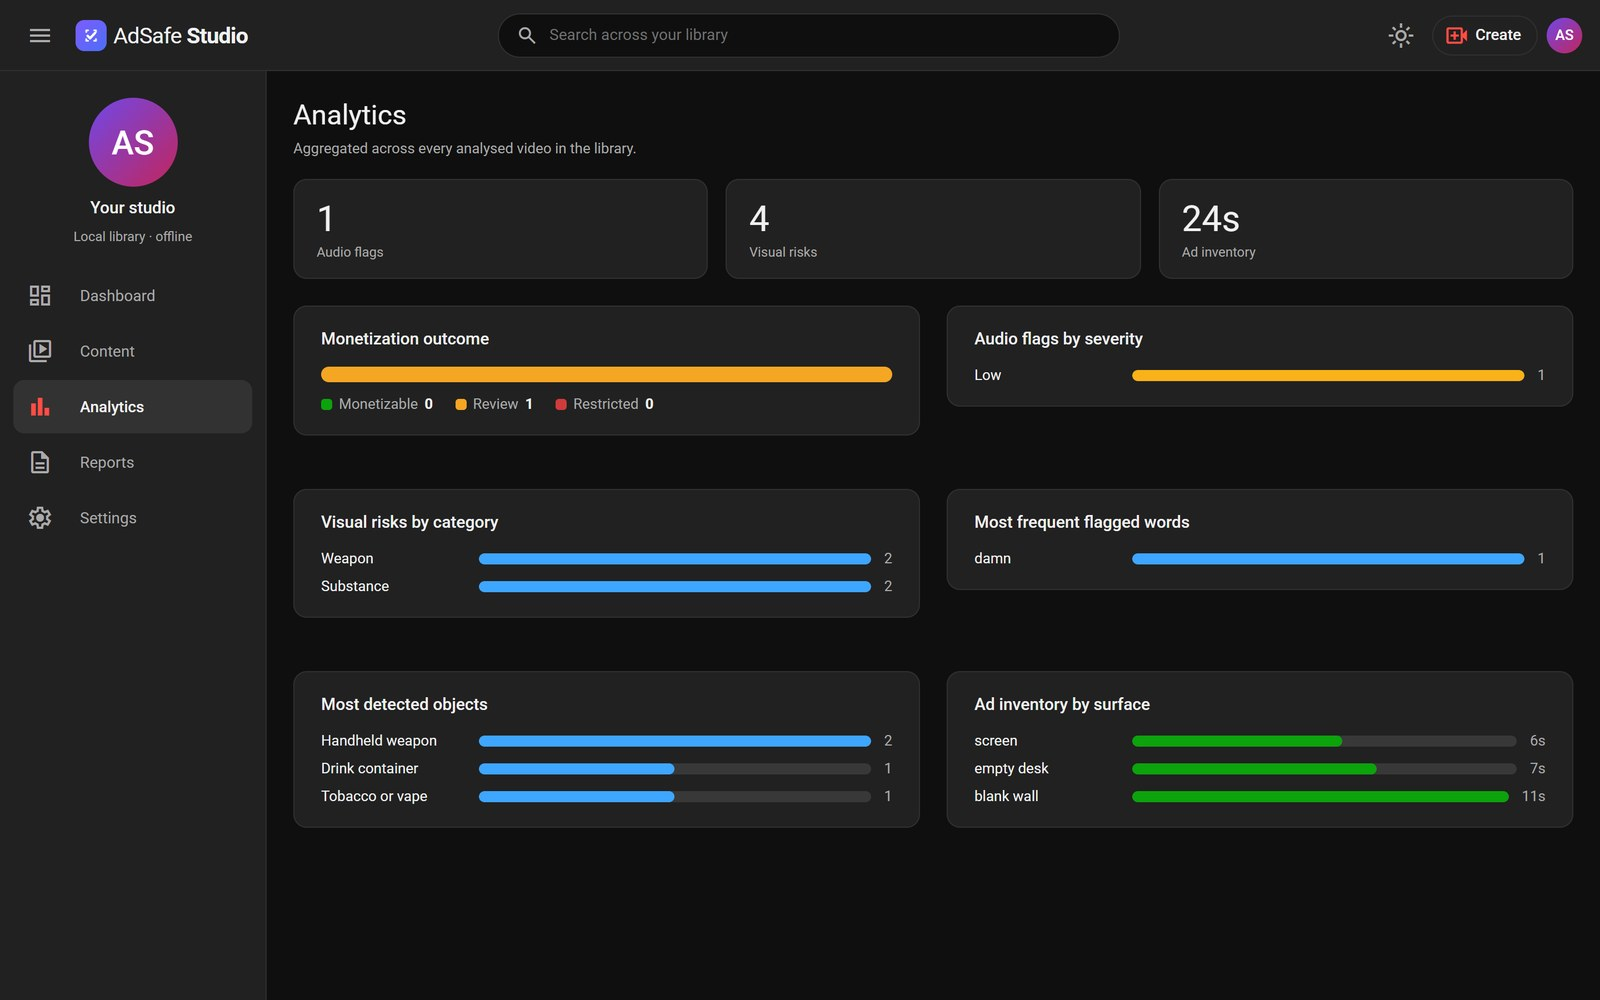
\includegraphics[width=0.95\textwidth]{Images/04-analytics.jpg}
\caption{Analytics: aggregate reporting across the library}
\end{figure}

The analytics view aggregates findings across every analysed video: the
monetisation outcome split, audio flags by severity, visual risks by category,
the most frequently flagged words, the most frequently detected objects, and
advertisement inventory by surface type. Objects are reported by their grouped
display label, so ``Handheld weapon'' appears rather than the individual model
classes.

\section{Operational Reports}

Three report types are produced per video, each recorded in the
\texttt{AuditReports} table with its type, path, finding counts and the
compliance status at the time of generation.

\begin{itemize}[itemsep=3pt]
\item \textbf{PDF} --- a formatted audit document for circulation, containing the
verdict, its reasoning, and the full finding tables.
\item \textbf{CSV} --- a flat export of findings for spreadsheet analysis.
\item \textbf{JSON} --- the complete structured result, including bounding boxes
and confidence scores, for programmatic use.
\end{itemize}

\section{Sample Report Layout}

\begin{figure}[H]
\centering
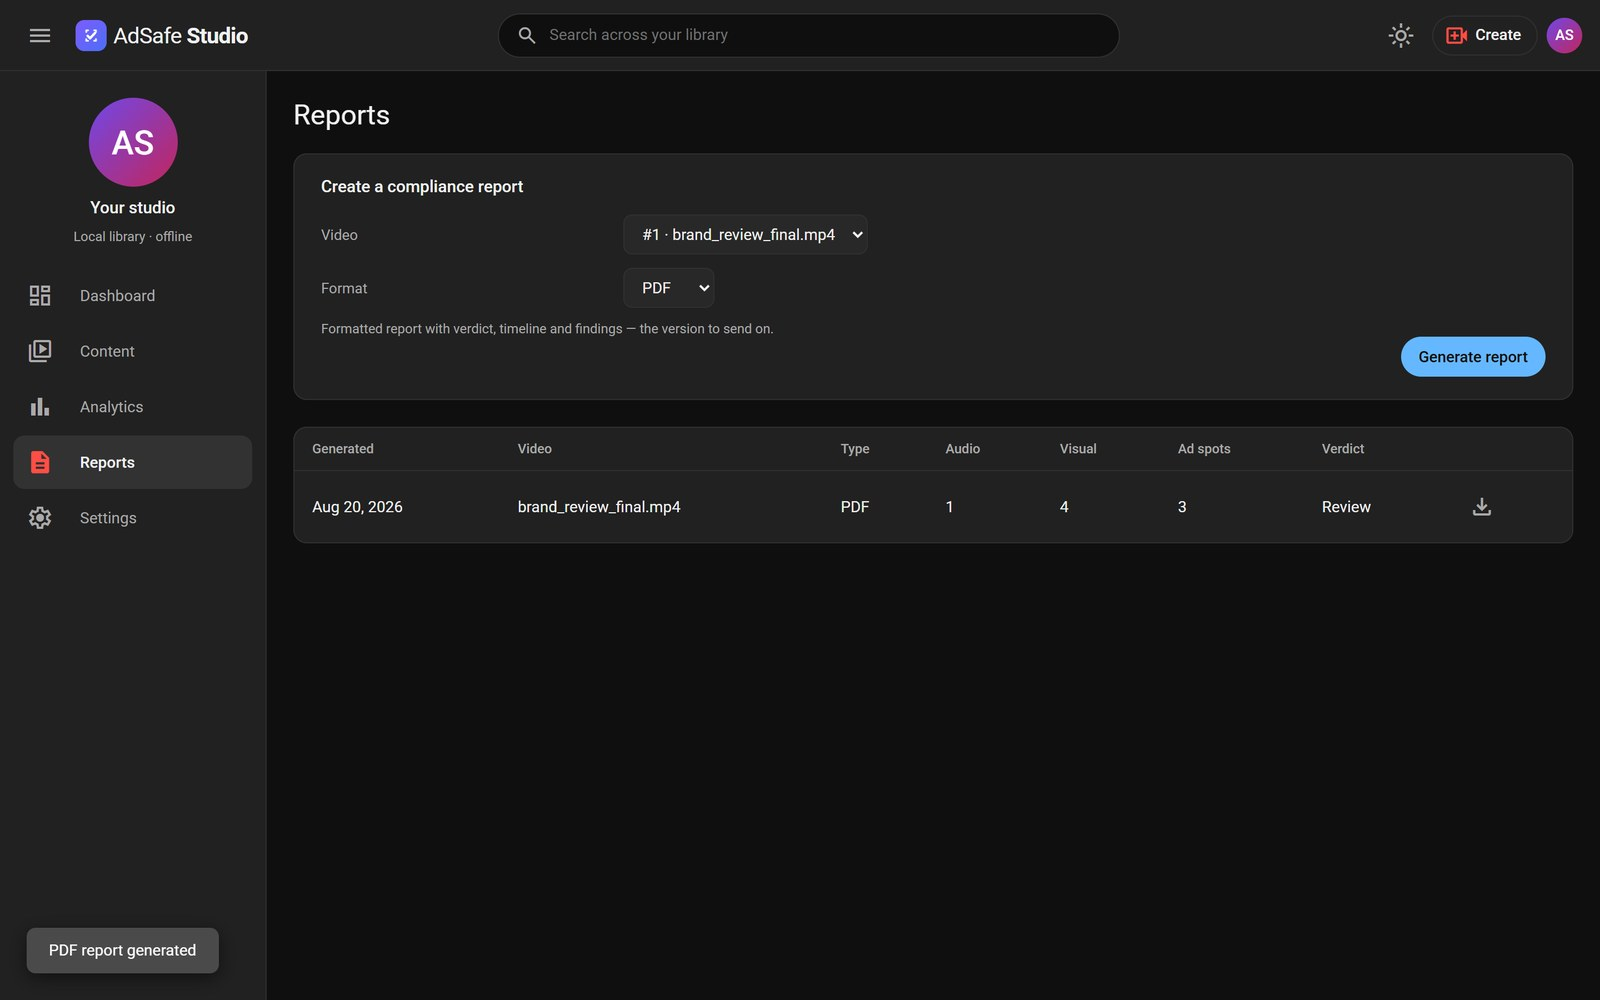
\includegraphics[width=0.95\textwidth]{Images/05-reports.jpg}
\caption{Reports screen with generation history}
\end{figure}

A generated report records the video and its metadata; the compliance verdict
with the reasoning that produced it; audio findings with timestamp, term,
severity, transcript context and producing engine; visual findings with
timestamp, grouped label, model class, confidence and producing engine;
advertisement surfaces with time range, bounding box and suitability score; and
the overlay-context evidence where present.

\section{Export Formats}

\begin{table}[H]
\centering
\begin{tabular}{|c|p{4.4cm}|p{5.6cm}|}
\hline
\textbf{Format} & \textbf{Produced with} & \textbf{Intended use} \\
\hline
PDF & ReportLab & Circulation, submission, archival record \\
\hline
CSV & pandas & Spreadsheet analysis, filtering, sorting \\
\hline
JSON & Standard library & Programmatic use; retains boxes and confidences \\
\hline
\end{tabular}
\caption{Export Formats}
\end{table}

\section{Output Screens}

\subsection{Video Detail and Audit Timeline}

\begin{figure}[H]
\centering
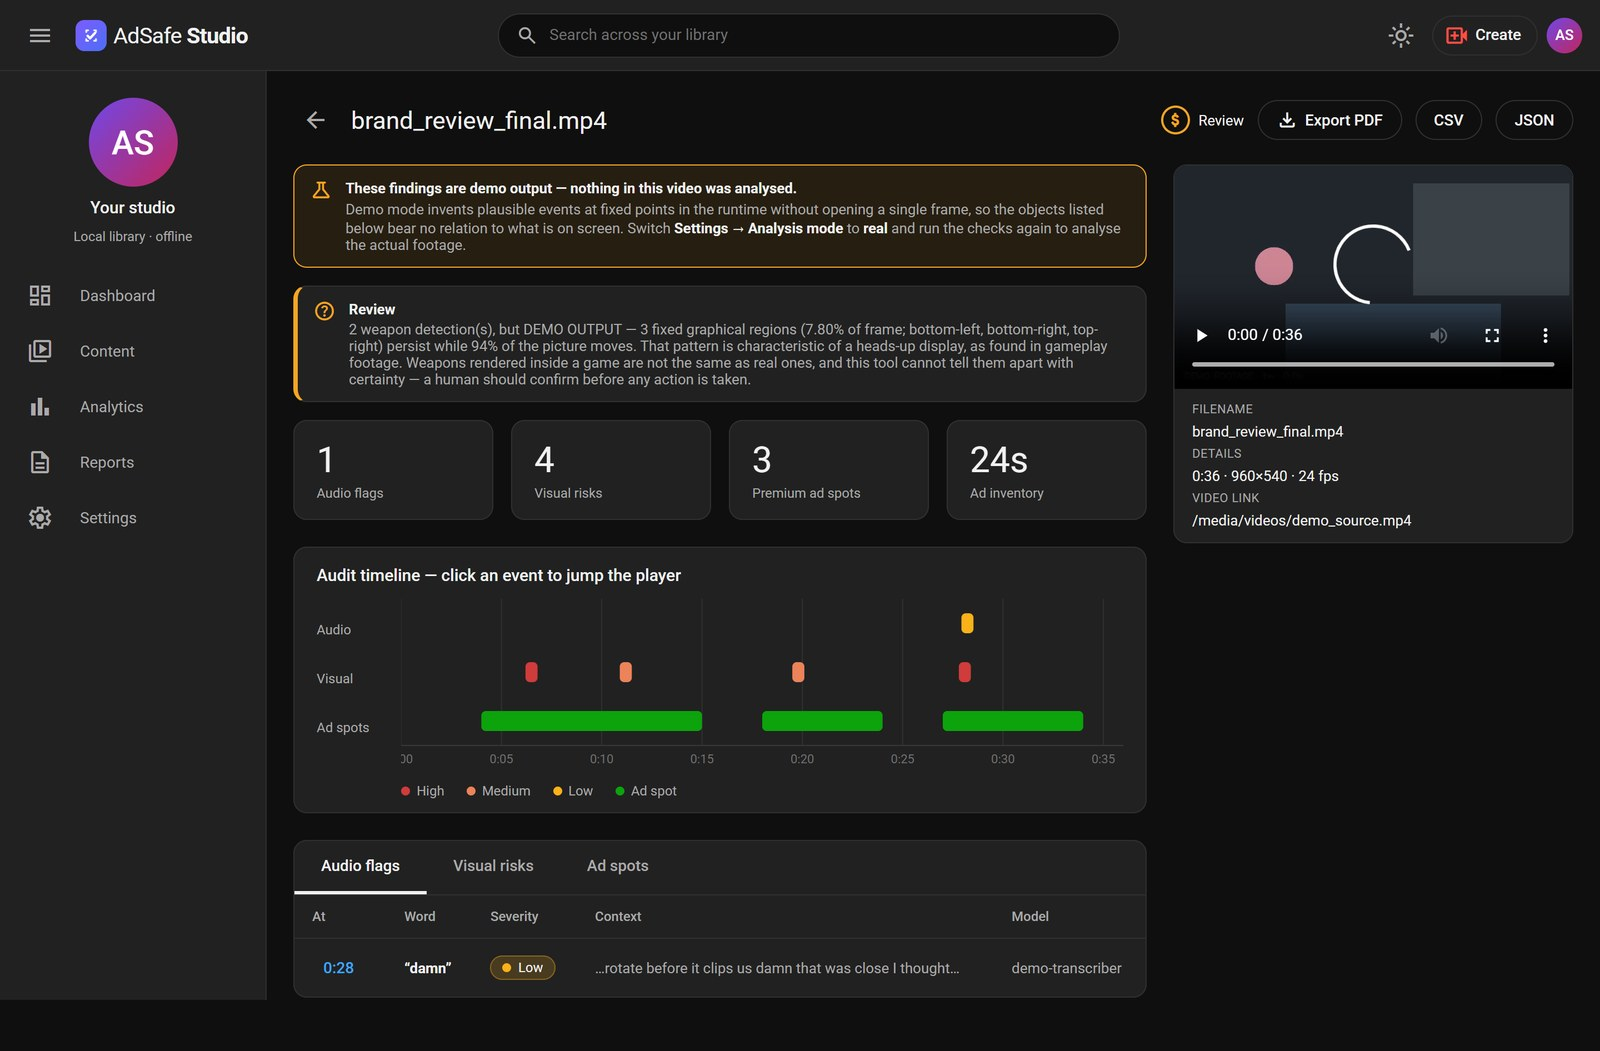
\includegraphics[width=0.95\textwidth]{Images/03-video-detail.jpg}
\caption{Video detail: verdict, reasoning, timeline and per-finding provenance}
\end{figure}

\subsection{Analysis in Progress}

\begin{figure}[H]
\centering
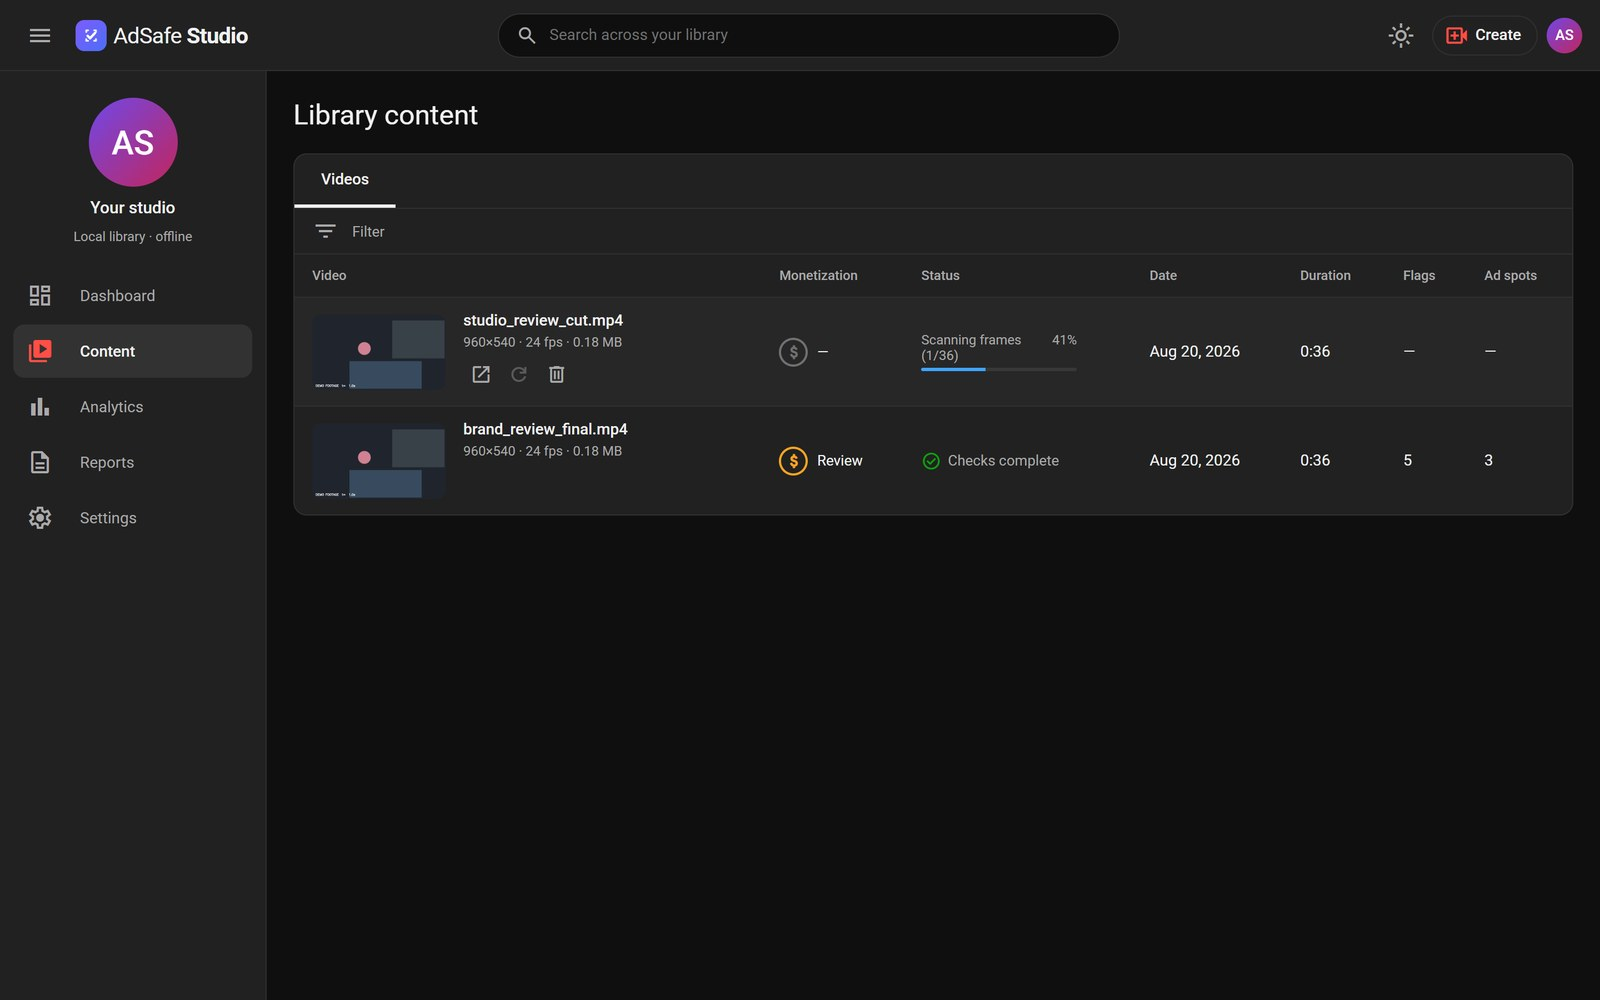
\includegraphics[width=0.95\textwidth]{Images/08-progress.jpg}
\caption{Inline progress during a real-mode analysis}
\end{figure}

\subsection{Settings and Detection Coverage}

\begin{figure}[H]
\centering
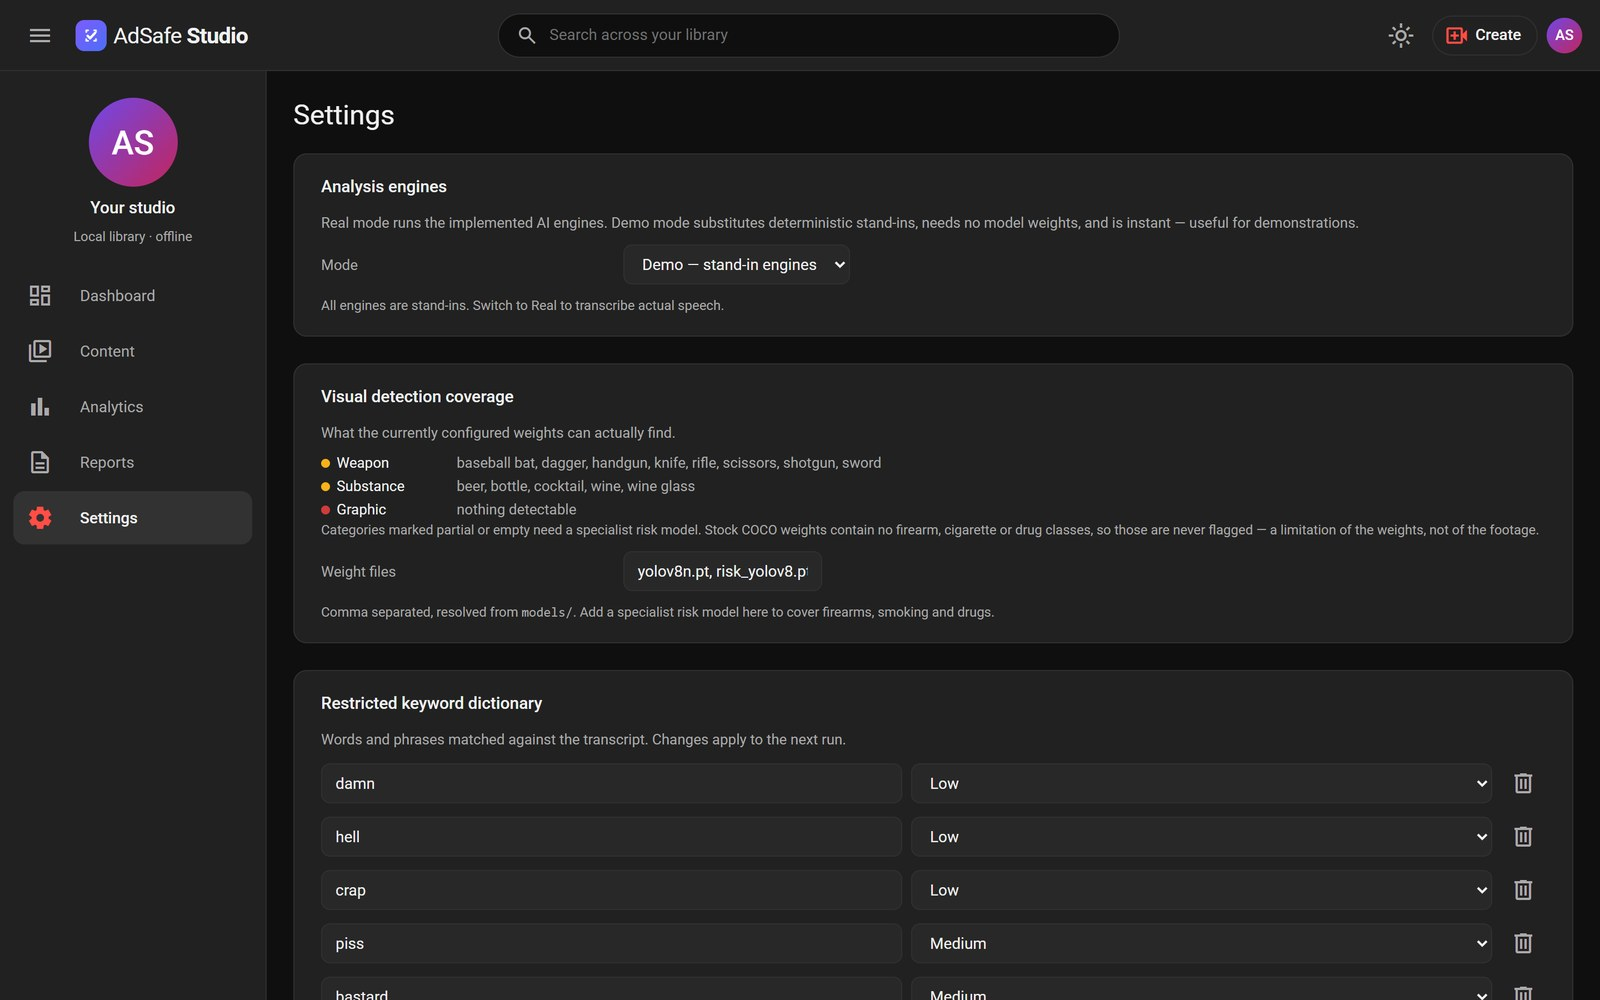
\includegraphics[width=0.95\textwidth]{Images/06-settings.jpg}
\caption{Settings: restricted vocabulary and pipeline configuration}
\end{figure}

The settings screen states what the loaded weights can and cannot detect, rather
than leaving the user to infer coverage from absence of findings. Categories the
models cannot detect are marked as such explicitly.

\subsection{Upload and Empty State}

\begin{figure}[H]
\centering
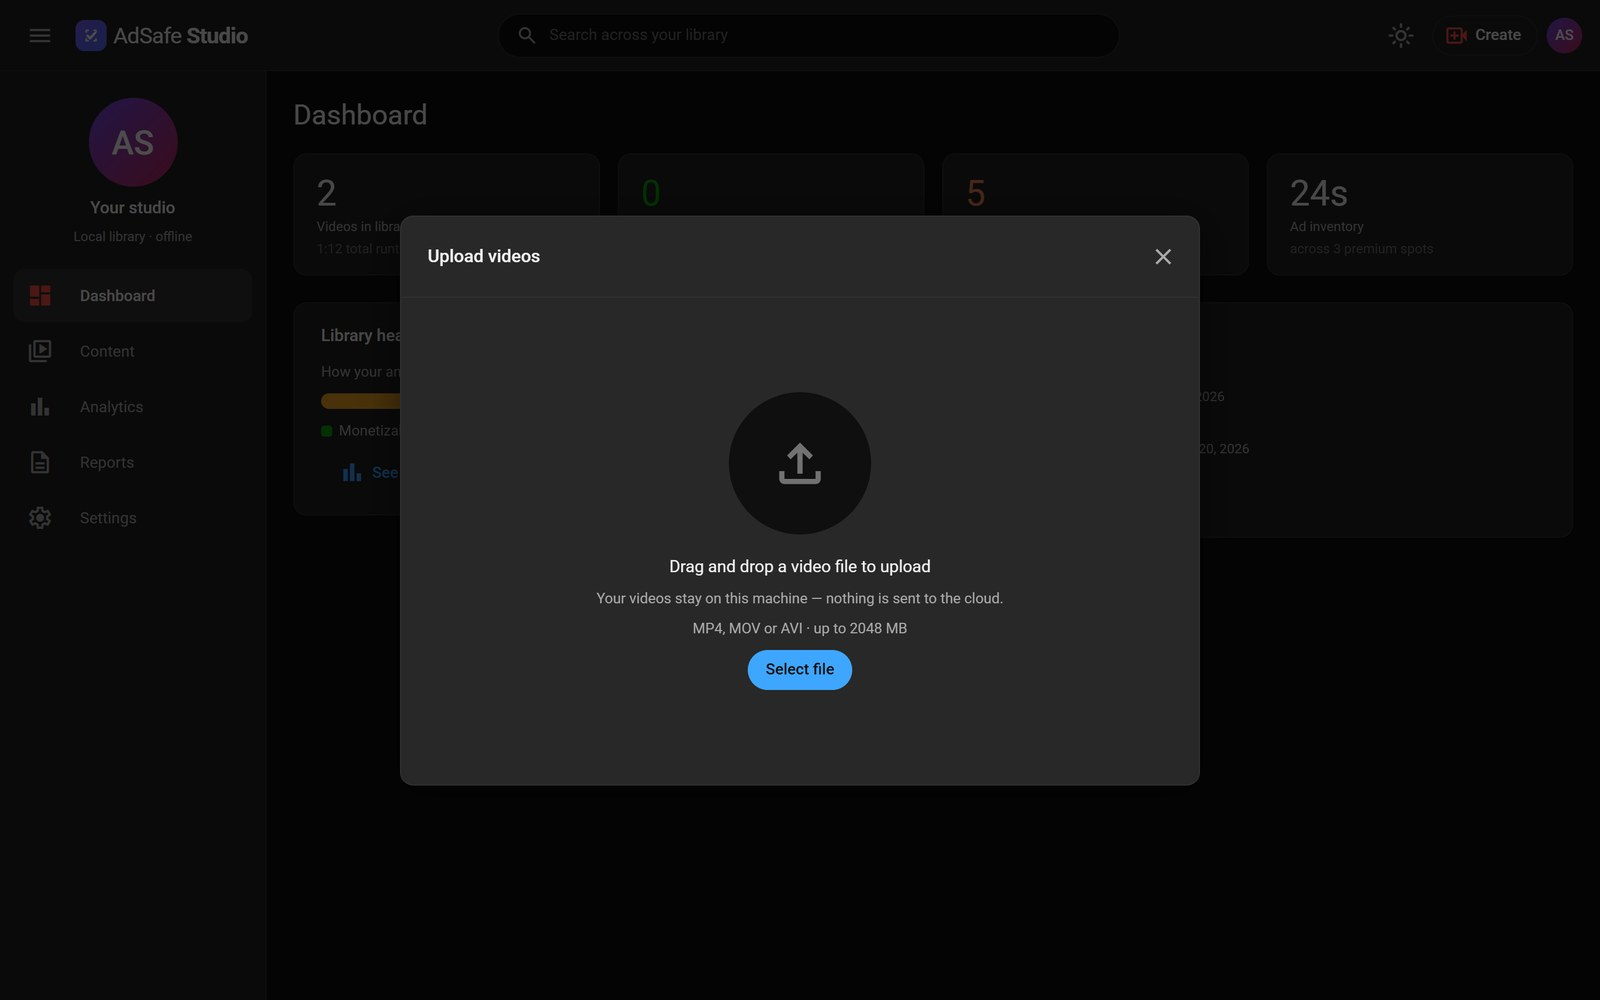
\includegraphics[width=0.47\textwidth]{Images/07-upload-dialog.jpg}
\hspace{0.2cm}
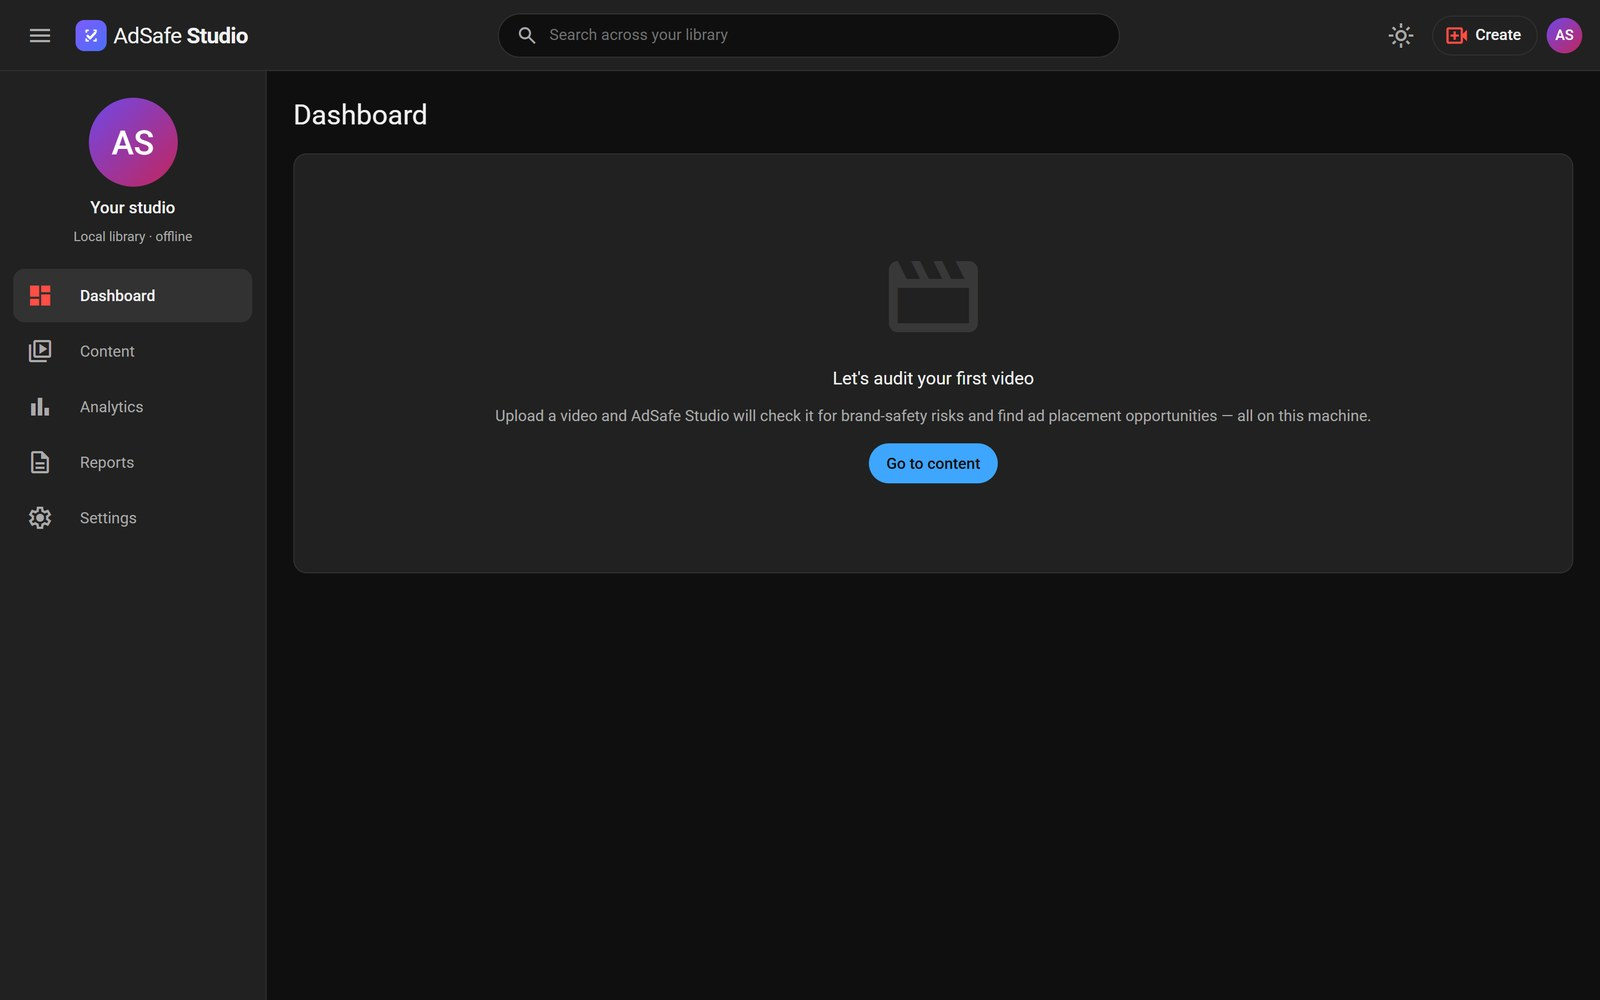
\includegraphics[width=0.47\textwidth]{Images/10-empty-state.jpg}
\caption{Upload dialog and first-run empty state}
\end{figure}

%%%%%%%%%%%%%%%%%%%%%%%%%%%%%%%%%%%%%%%%%%%%%%%%%%
\chapter{Conclusion and Future Scope}
%%%%%%%%%%%%%%%%%%%%%%%%%%%%%%%%%%%%%%%%%%%%%%%%%%

\section{Conclusion}

The project set out to build a pre-publication advertiser-suitability check that
runs on a creator's own machine and explains its findings. That system exists
and works.

All eight stated objectives were met. A video can be ingested and its metadata
stored; its speech is transcribed with word-level timestamps and matched against
a configurable vocabulary; its frames are scanned by a detection model trained
specifically for this project's risk taxonomy; unoccupied regions of the frame
are located and reported as advertisement inventory; persistent overlays are
detected so that rendered content is weighed differently from filmed content; a
three-state verdict is produced with its reasoning attached; findings are
presented on a navigable timeline and exported in three formats; and the entire
analysis runs locally, with the absence of any external network request verified
automatically rather than asserted.

Three results are worth carrying forward beyond this report.

\textbf{Validation metrics did not predict behaviour on video, and this was
demonstrated twice.} A fine-tuning run that improved almost every headline
metric detected a real firearm zero times where its predecessor detected it
thirteen times. Any model change in work of this kind must be gated on the
target medium, not on a held-out split of the training distribution.

\textbf{Class definition mattered more than class volume.} The class with the
most training data scored worst and the class with the least scored
substantially better, because the labels in the source dataset overlapped in the
first case and were clean in the second.

\textbf{Real footage found defects that synthetic testing could not.} Four real
clips produced four distinct failures, each of which had passed every automated
test in place at the time.

\section{Limitations}

\begin{enumerate}[itemsep=3pt]
\item \textbf{No accuracy figure is claimed on creator footage.} The benchmark
corpus is unlabelled, so precision and recall on real video are unmeasured.
\item \textbf{Detection is limited to the trained taxonomy.} Smoking and
narcotics are not detected visually, because the source dataset supplies no
usable classes for them; they are covered in the audio vocabulary only.
\item \textbf{The specific weapon class is unreliable} even though the category
is not, which is why findings are reported as grouped terms.
\item \textbf{The overlay detector detects overlays, not games.} A watermark or
a lower-third will also be detected; region count and coverage are reported so
that a single corner region reads as a watermark rather than a heads-up display.
\item \textbf{No authentication, and no upload size limit.} Both follow from the
single-user local model, and both would need to be addressed before any network
exposure.
\item \textbf{The system does not predict any specific platform's decision.} It
is an advisory tool, and deliberately does not claim to replicate a proprietary
classifier.
\end{enumerate}

\section{Future Scope}

\begin{enumerate}[itemsep=3pt]
\item \textbf{Complete the labelled benchmark corpus.} Twenty real clips with
labelled events would allow a measured precision figure to replace the withdrawn
claim. This is the single highest-value remaining task.
\item \textbf{Suppress advertisement surfaces inside detected overlay regions.}
A heads-up display is stable and uncluttered, so it scores well as an
advertisement surface while being the worst possible place to put one.
\item \textbf{Extend the risk taxonomy} to smoking and narcotics using a dataset
that supplies usable classes for them.
\item \textbf{A third fine-tuning run} with a single controlled change,
evaluated on video rather than on validation metrics.
\end{enumerate}

\section{Further Enhancements}

\begin{enumerate}[itemsep=3pt]
\item Batch analysis across an entire library rather than one video at a time.
\item Export of the audit timeline as an image for inclusion in reports.
\item Per-video content-type declaration --- Gaming, Education, News --- to
complement the overlay heuristic, mirroring how platforms allow creators to
self-certify.
\item Upload size limits and configurable storage quotas.
\item GPU acceleration where a compatible device is present, with automatic
fallback to CPU.
\end{enumerate}

%%%%%%%%%%%%%%%%%%%%%%%%%%%%%%%%%%%%%%%%%%%%%%%%%%
% APPENDICES
%%%%%%%%%%%%%%%%%%%%%%%%%%%%%%%%%%%%%%%%%%%%%%%%%%

\appendix

\chapter{Source Code}

Selected modules are reproduced here. The complete source is in the project
repository.

\section{Compliance Verdict Determination}

\begin{lstlisting}[language=Python, caption={Three-state verdict with reasoning
(src/pipeline/orchestrator.py, abridged)}]
def assess_compliance(video_id):
    """Return the verdict AND the reasoning that produced it.

    A verdict the interface cannot explain is no more accountable than the
    binary label it was built to replace.
    """
    audio = repo.get_audio_flags(video_id)
    visual = repo.get_visual_flags(video_id)
    overlay = repo.get_overlay_context(video_id)

    reasons = []
    high = [a for a in audio if a["severity"] == "High"]
    weapons = [v for v in visual if v["risk_category"] == "Weapon"]

    if high:
        reasons.append(f"{len(high)} unambiguous restricted term(s).")
        verdict = "Restricted"
    elif weapons and overlay and overlay["is_overlay"]:
        # Rendered, not filmed: report it, but do not restrict on it.
        reasons.append(
            f"{len(weapons)} weapon detection(s), but {overlay['regions']} "
            f"fixed graphical regions persist while the picture moves. "
            "That pattern is characteristic of a heads-up display.")
        verdict = "Review"
    elif weapons:
        reasons.append(f"{len(weapons)} weapon detection(s) in filmed content.")
        verdict = "Restricted"
    ...
    return {"verdict": verdict, "reasoning": " ".join(reasons)}
\end{lstlisting}

\section{Free-Space Advertisement Surface Detection}

\begin{lstlisting}[language=Python, caption={Largest all-clear rectangle
(src/vision/adspots.py, abridged)}]
def largest_clear_rectangle(occupancy):
    """Maximal rectangle of zeros in a binary matrix, in O(rows x cols).

    A blank wall is the ABSENCE of objects, so this cannot be learned by a
    detector -- it is a classical scan over the occupancy matrix instead.
    """
    rows, cols = occupancy.shape
    heights = [0] * cols
    best = (0, None)
    for r in range(rows):
        for c in range(cols):
            heights[c] = 0 if occupancy[r][c] else heights[c] + 1
        area, box = _largest_in_histogram(heights, r)
        if area > best[0]:
            best = (area, box)
    return best
\end{lstlisting}

\section{Upload Path Safety}

\begin{lstlisting}[language=Python, caption={Directory-traversal fix
(backend/routes/videos.py)}]
# .name strips any directory part the client sent. Interpolating the raw
# filename let it escape VIDEO_DIR: "a/../../../../evil.mp4" normalises to a
# path outside the repository, and the suffix check still saw ".mp4" because
# only the last component is inspected.
original = Path(file.filename or "upload.mp4").name
suffix = Path(original).suffix.lower()
if suffix not in config.SUPPORTED_EXTENSIONS:
    raise HTTPException(400, f"Unsupported format {suffix}.")
dest = config.VIDEO_DIR / f"{stamp}_{original}"
\end{lstlisting}

\chapter{User Manual}

\section{Installation}

\begin{lstlisting}[caption={One-time setup}]
git clone <repository-url>
cd specproj
pip install -r requirements.txt
npm install --prefix frontend
npm run build --prefix frontend
\end{lstlisting}

\section{Running the Application}

On Windows, double-click \texttt{RUN\_DEMO.bat}. It builds the interface if
required, refuses to start a second server on an occupied port, starts the
application and opens a browser at \texttt{http://localhost:8000}.

Equivalently, from a terminal:

\begin{lstlisting}
python -m uvicorn backend.main:app --port 8000
\end{lstlisting}

\section{Analysing a Video}

\begin{enumerate}[itemsep=3pt]
\item Click \textbf{Create} and choose a file, or drag it onto the drop zone.
MP4, MOV and AVI are accepted.
\item On the \textbf{Content} screen, hover the row and click \textbf{Run
checks}. Progress is reported inline with the current stage.
\item When the run completes, click the video title to open its detail screen.
\item Read the verdict and its reasoning at the top of the page. Click any
marker on the audit timeline to seek the player to that moment.
\item Use the \textbf{Audio flags}, \textbf{Visual risks} and \textbf{Ad spots}
tabs to review findings in detail. The \textbf{Model} column records which
engine produced each finding.
\item Export with \textbf{Export PDF}, \textbf{CSV} or \textbf{JSON}.
\end{enumerate}

\section{Demonstration and Real Modes}

The application ships in \textbf{demonstration mode}, which produces plausible
findings instantly without opening a single frame. It exists so the interface
can be shown without waiting for a real analysis.

\textbf{Demonstration output is not measurement}, and the application says so in
several places: an amber banner on any video analysed in demonstration mode, and
the producing engine recorded against every individual finding. To analyse real
footage, set \textbf{Settings $\rightarrow$ Analysis mode} to \textbf{real} and
run the checks again.

\section{Configuration}

The settings screen exposes the restricted vocabulary with per-term severity,
the frame sample rate, the minimum advertisement-spot duration, the detection
confidence threshold and the detection resolution cap. Each field states its
trade-off in the interface.

\chapter{Database Scripts}

\begin{lstlisting}[language=SQL, caption={Schema}]
PRAGMA journal_mode = WAL;
PRAGMA foreign_keys = ON;

CREATE TABLE VideoMetadata (
    video_id            INTEGER PRIMARY KEY AUTOINCREMENT,
    filename            TEXT NOT NULL,
    filepath            TEXT NOT NULL,
    file_size_mb        REAL NOT NULL,
    duration_sec        REAL NOT NULL,
    fps                 REAL NOT NULL,
    resolution_width    INTEGER,
    resolution_height   INTEGER,
    upload_timestamp    TEXT DEFAULT CURRENT_TIMESTAMP,
    processed_status    TEXT DEFAULT 'pending'
                        CHECK (processed_status IN
                              ('pending','processing','completed','failed')),
    overlay_context     TEXT
);

CREATE TABLE AudioFlags (
    audio_flag_id       INTEGER PRIMARY KEY AUTOINCREMENT,
    video_id            INTEGER NOT NULL
                        REFERENCES VideoMetadata(video_id) ON DELETE CASCADE,
    timestamp_start     REAL NOT NULL,
    timestamp_end       REAL NOT NULL,
    word_flagged        TEXT NOT NULL,
    transcript_context  TEXT,
    severity            TEXT CHECK (severity IN ('Low','Medium','High')),
    detection_model     TEXT DEFAULT 'faster-whisper-base.en'
);

CREATE TABLE VisualFlags (
    visual_flag_id      INTEGER PRIMARY KEY AUTOINCREMENT,
    video_id            INTEGER NOT NULL
                        REFERENCES VideoMetadata(video_id) ON DELETE CASCADE,
    frame_timestamp     REAL NOT NULL,
    object_detected     TEXT NOT NULL,
    bounding_box_json   TEXT NOT NULL,
    confidence_score    REAL NOT NULL,
    risk_category       TEXT CHECK (risk_category IN
                                   ('Weapon','Substance','Graphic')),
    detection_model     TEXT
);

CREATE TABLE AdSpots (
    spot_id             INTEGER PRIMARY KEY AUTOINCREMENT,
    video_id            INTEGER NOT NULL
                        REFERENCES VideoMetadata(video_id) ON DELETE CASCADE,
    timestamp_start     REAL NOT NULL,
    timestamp_end       REAL NOT NULL,
    spot_type           TEXT,
    bounding_box_json   TEXT NOT NULL,
    area_pixels         REAL,
    suitability_score   REAL
);

CREATE TABLE AuditReports (
    report_id             INTEGER PRIMARY KEY AUTOINCREMENT,
    video_id              INTEGER NOT NULL
                          REFERENCES VideoMetadata(video_id) ON DELETE CASCADE,
    generation_timestamp  TEXT DEFAULT CURRENT_TIMESTAMP,
    report_type           TEXT CHECK (report_type IN ('PDF','CSV','JSON')),
    file_path             TEXT,
    total_audio_risks     INTEGER,
    total_visual_risks    INTEGER,
    total_ad_spots        INTEGER,
    compliance_status     TEXT
);

CREATE TABLE SystemConfig (
    config_key      TEXT PRIMARY KEY,
    config_value    TEXT NOT NULL,
    config_type     TEXT CHECK (config_type IN
                               ('string','int','float','json')),
    description     TEXT,
    last_updated    TEXT DEFAULT CURRENT_TIMESTAMP
);
\end{lstlisting}

\chapter{Additional Screenshots}

\begin{figure}[H]
\centering
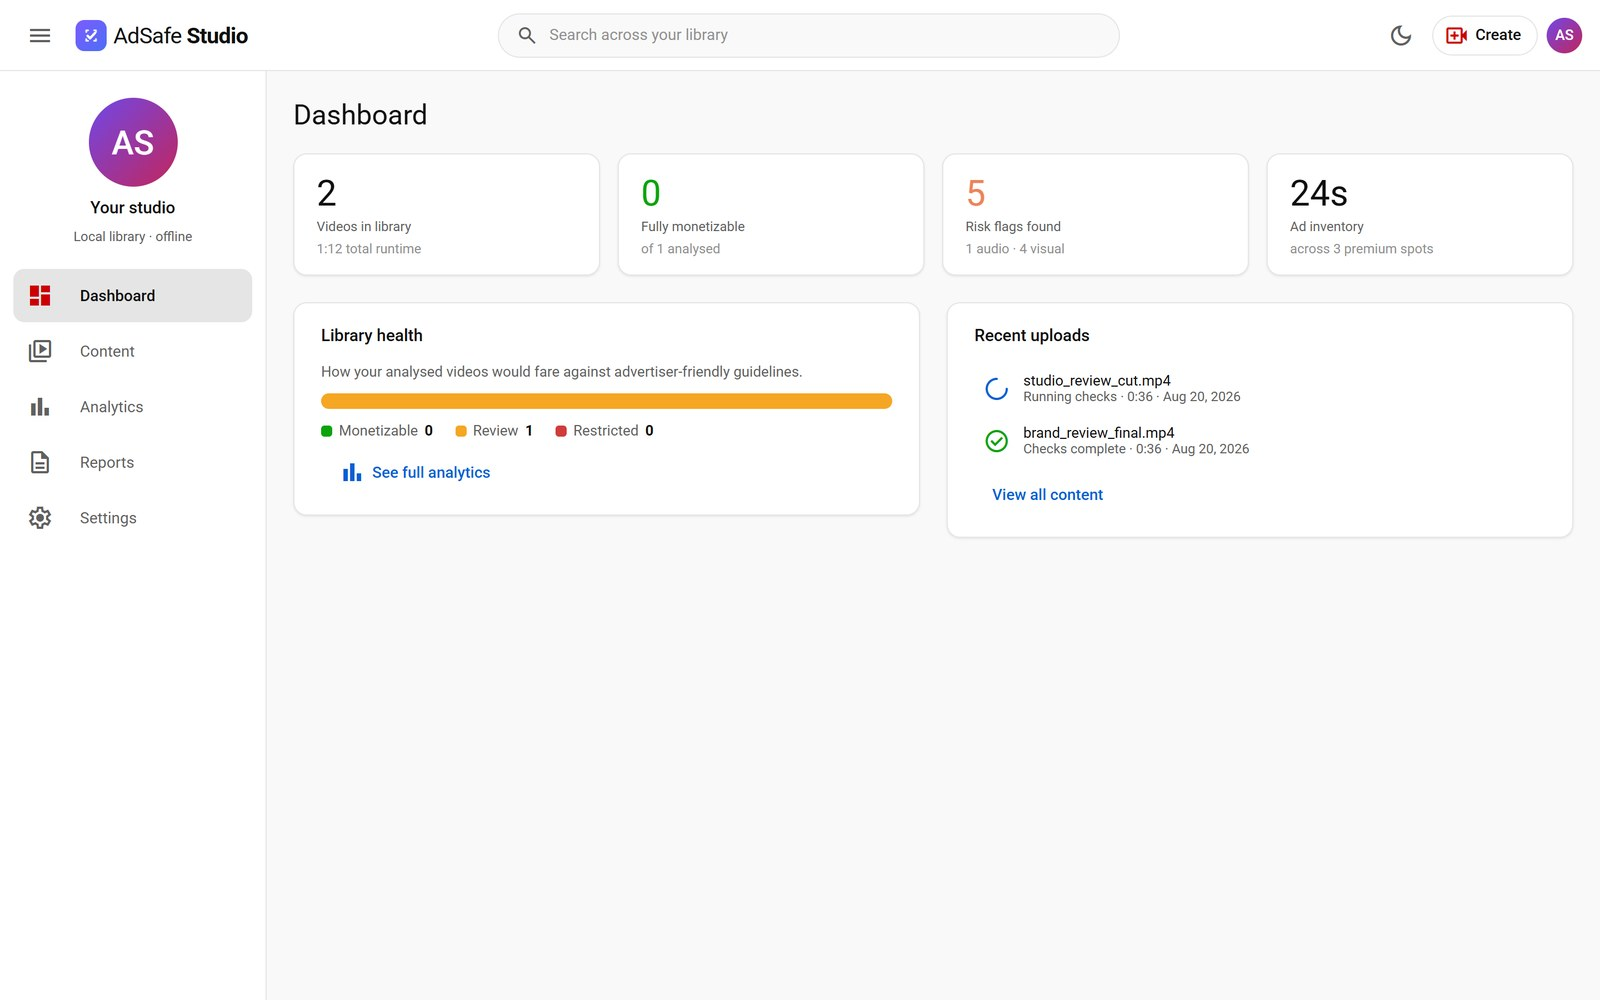
\includegraphics[width=0.95\textwidth]{Images/14-theme-light.jpg}
\caption{Light theme, demonstrating the design token system}
\end{figure}

\begin{figure}[H]
\centering
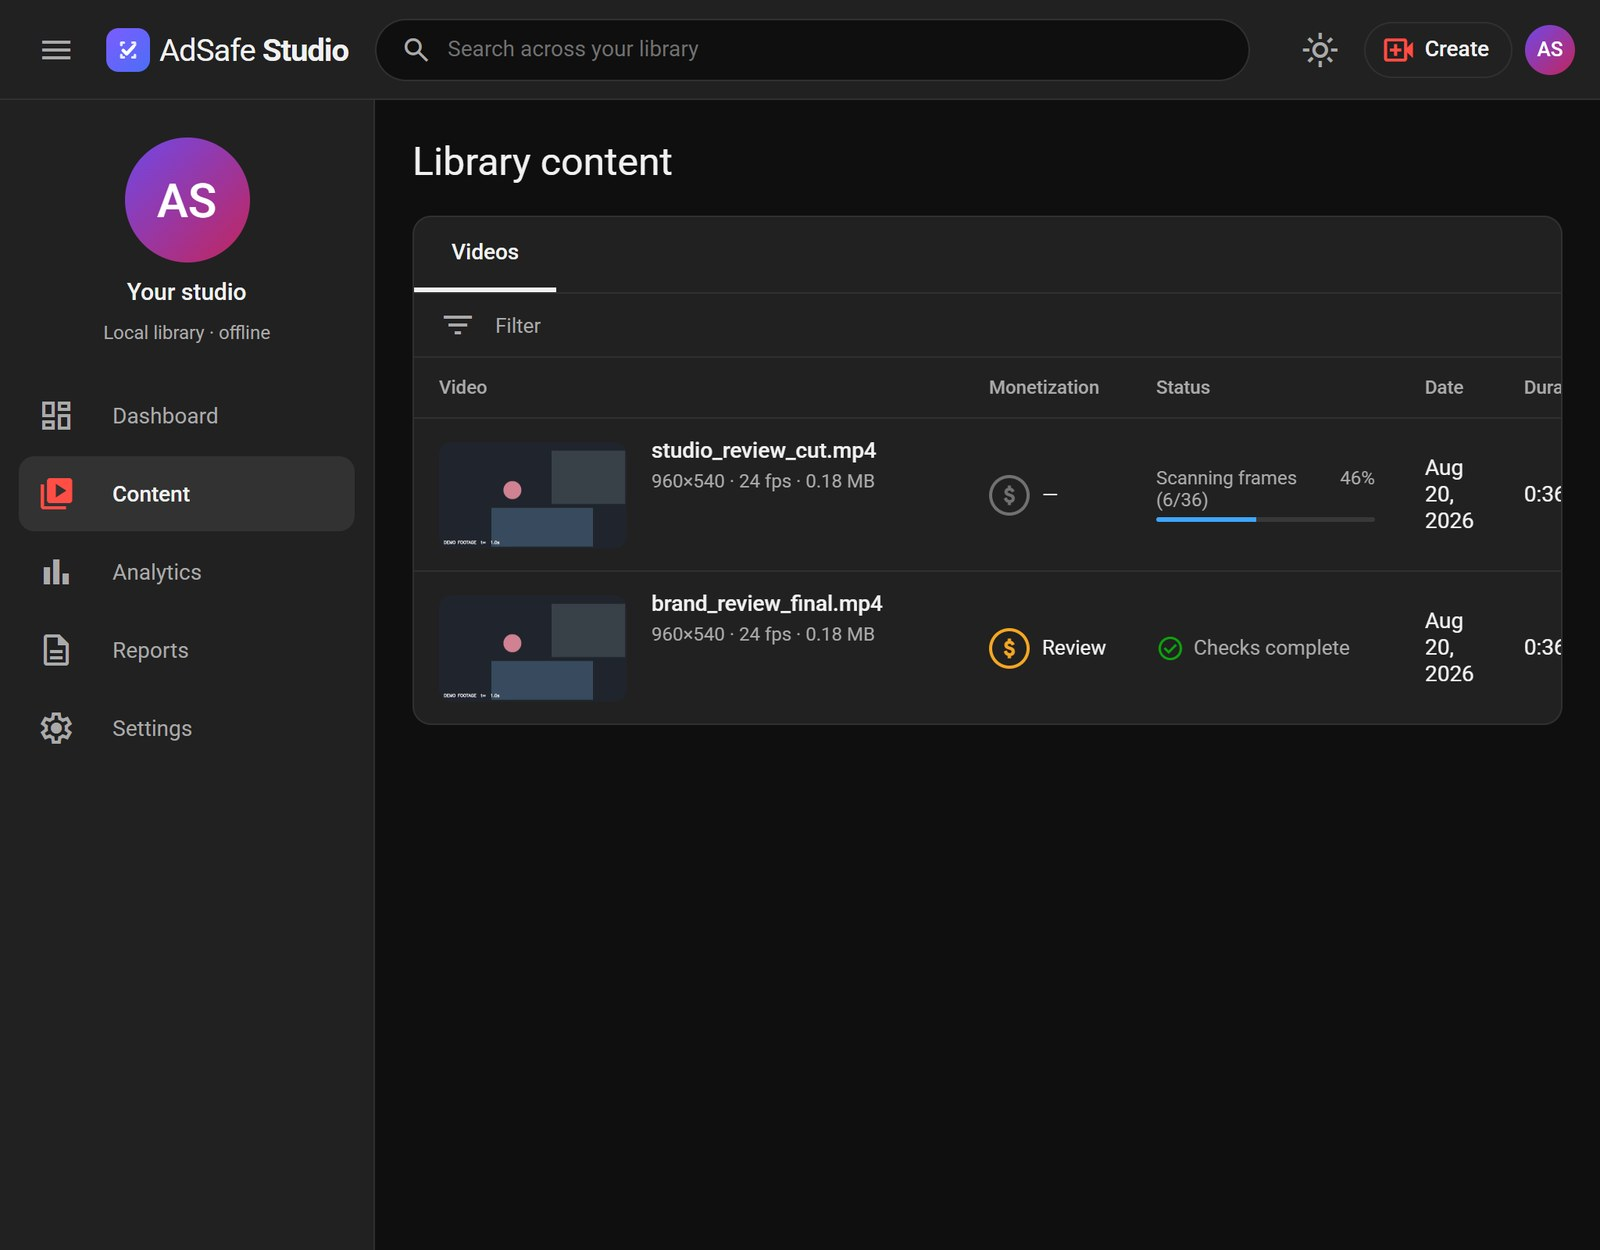
\includegraphics[width=0.95\textwidth]{Images/11-responsive-laptop.jpg}
\caption{Laptop width, 1024\,px: navigation collapsed to an icon rail}
\end{figure}

\chapter{Project Artefacts}

\section{Data Flow Diagram Level 1}

\begin{figure}[H]
\centering
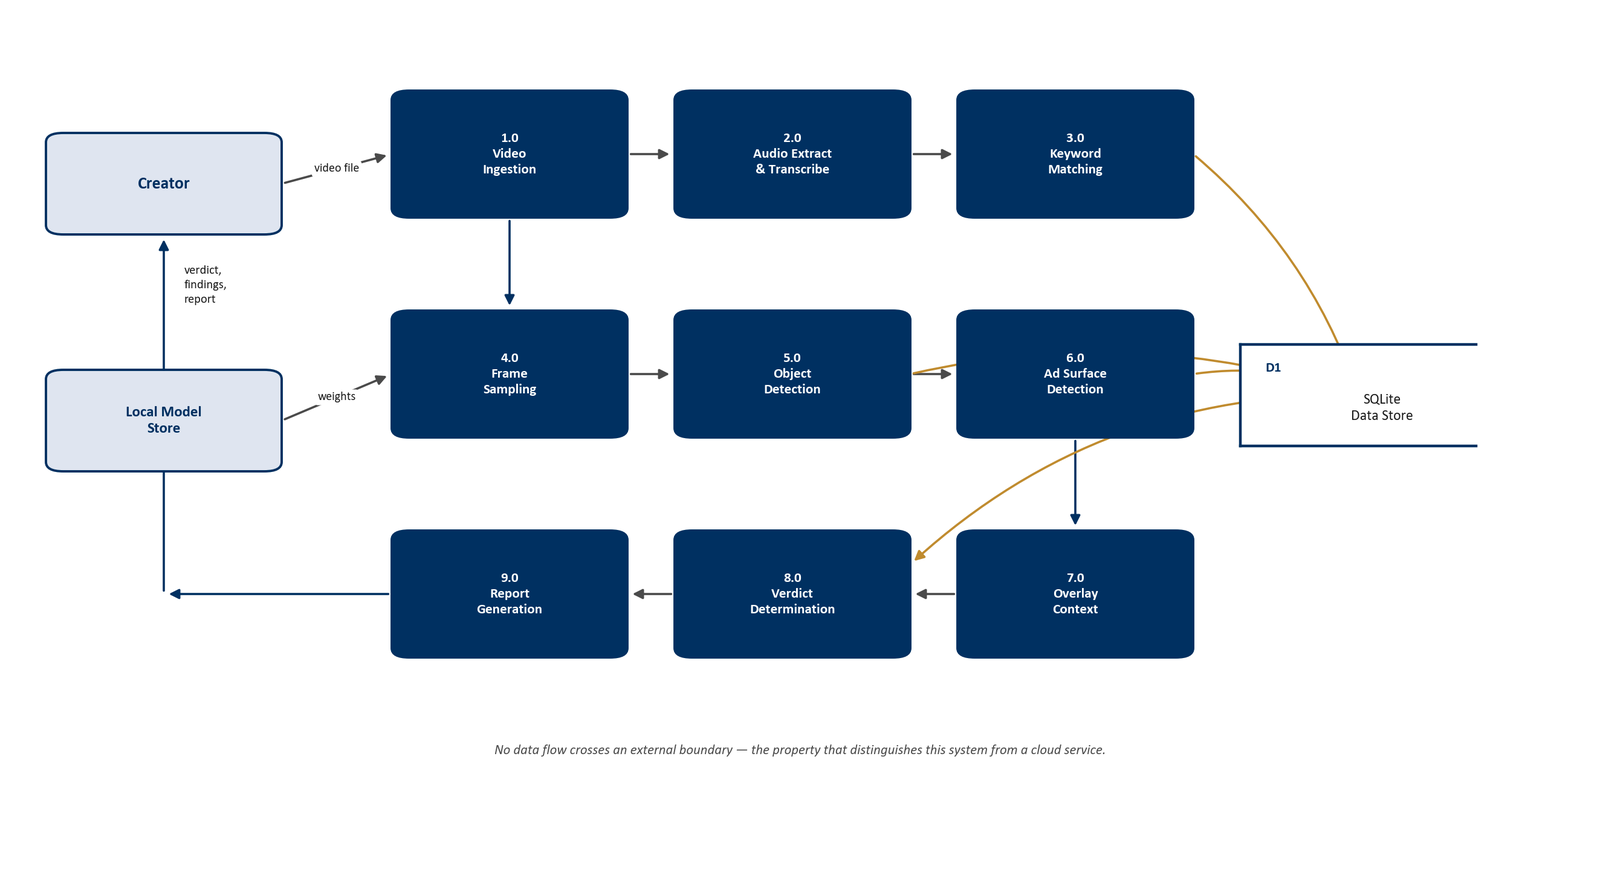
\includegraphics[width=0.95\textwidth]{Images/dfd_level1.png}
\caption{Level 1 data flow, reproduced for reference}
\end{figure}

\section{Repository and Engineering Record}

Every change is recorded as a separate commit whose message states what changed
and why, including the defects described in Chapter~8 and
Chapter~\ref{ch:security}. The repository therefore serves as the detailed
engineering record supporting this report.

\section{Supporting Tooling}

\begin{table}[H]
\centering
\begin{tabular}{|p{5.4cm}|p{7.4cm}|}
\hline
\textbf{Tool} & \textbf{Purpose} \\
\hline
\texttt{docs/diagrams/make\_diagrams.py} & Generates all fourteen diagrams in
this report from code, so they cannot drift from the system \\
\hline
\texttt{docs/capture\_screens.py} & Captures every interface screenshot and
checks all six pages at five widths for layout overflow \\
\hline
\texttt{docs/check\_offline.py} & Severs all non-local traffic and verifies the
interface still renders \\
\hline
\texttt{benchmark/status.py} & Reports benchmark coverage against its gates and
refuses to publish an unsupported figure \\
\hline
\texttt{demo\_setup.py} & Resets the demonstration library, refusing to delete
anything if the database is locked \\
\hline
\end{tabular}
\caption{Supporting tooling}
\end{table}

%%%%%%%%%%%%%%%%%%%%%%%%%%%%%%%%%%%%%%%%%%%%%%%%%%
% GLOSSARY
%%%%%%%%%%%%%%%%%%%%%%%%%%%%%%%%%%%%%%%%%%%%%%%%%%

\chapter*{Glossary}
\addcontentsline{toc}{chapter}{Glossary}

\begin{longtable}{p{4cm}p{9cm}}
Ad spot &
A region of the frame that stays unoccupied long enough to carry an overlay
advertisement \\

Bounding box &
The rectangle describing where a detected object sits within a frame \\

COCOMO &
Constructive Cost Model, an algorithmic software cost estimation model \\

Demonstration mode &
A mode that produces plausible findings instantly without analysing frames,
used only for demonstration and labelled as such throughout the interface \\

Fine-tuning &
Further training of a pretrained model on a task-specific dataset \\

HUD &
Heads-up display; the persistent on-screen graphics of a video game \\

IoU &
Intersection over Union; the overlap measure used to merge duplicate detections
\\

mAP@50 &
Mean average precision at an IoU threshold of 0.50 \\

Maximal rectangle &
The largest all-clear rectangle within a binary occupancy matrix \\

Overlay context &
Evidence that part of the frame is rendered rather than filmed, derived from
per-pixel temporal variance \\

Persistence threshold &
The minimum duration a clear surface must last to be reported as an ad spot \\

Verdict &
The three-state advertiser-suitability outcome: Monetizable, Review or
Restricted \\

WAL &
Write-Ahead Logging; a SQLite journal mode allowing reads concurrent with a
writer \\
\end{longtable}

%%%%%%%%%%%%%%%%%%%%%%%%%%%%%%%%%%%%%%%%%%%%%%%%%%
% SUBMISSION CHECKLIST
%%%%%%%%%%%%%%%%%%%%%%%%%%%%%%%%%%%%%%%%%%%%%%%%%%

\chapter*{Submission Checklist}
\addcontentsline{toc}{chapter}{Submission Checklist}

\begin{table}[H]
\centering
\begin{tabular}{|p{10cm}|c|}
\hline
\textbf{Item} & \textbf{Completed} \\
\hline
Title Page & Yes \\
\hline
Certificate & Yes \\
\hline
Declaration & Yes \\
\hline
Abstract & Yes \\
\hline
SRS (requirements, Chapters 1--2) & Yes \\
\hline
System Modeling (nine diagrams, Chapter 5) & Yes \\
\hline
Database Design (Chapter 6, Appendix C) & Yes \\
\hline
UI Design (Chapter 6) & Yes \\
\hline
Coding (Chapter 7, Appendix A) & Yes \\
\hline
Testing (Chapter 8, 175 tests) & Yes \\
\hline
Security Measures (Chapter 9) & Yes \\
\hline
Cost Estimation (Chapter 10) & Yes \\
\hline
Reports (Chapter 11) & Yes \\
\hline
References & Yes \\
\hline
Appendices (A--E) & Yes \\
\hline
Measured accuracy on labelled creator footage & \textbf{No --- see
Section~\ref{sec:accuracy}} \\
\hline
\end{tabular}
\caption{Project Submission Checklist}
\end{table}

%%%%%%%%%%%%%%%%%%%%%%%%%%%%%%%%%%%%%%%%%%%%%%%%%%
% REFERENCES
%%%%%%%%%%%%%%%%%%%%%%%%%%%%%%%%%%%%%%%%%%%%%%%%%%
% NOTE: the supplied template placed its bibliography AFTER \end{document} and
% never called \printbibliography, so no reference would ever have appeared.
% Keys match the \cite commands in the text and the entries in references.bib.

\addcontentsline{toc}{chapter}{References}
\begin{thebibliography}{99}

\bibitem{Sommerville2016}
I. Sommerville, \textit{Software Engineering}, 10th ed. Pearson Education,
2016.

\bibitem{Pressman2015}
R. S. Pressman, \textit{Software Engineering: A Practitioner's Approach},
8th ed. McGraw Hill, 2015.

\bibitem{Elmasri2017}
R. Elmasri and S. Navathe, \textit{Fundamentals of Database Systems}, 7th ed.
Pearson Education, 2017.

\bibitem{Gamma1994}
E. Gamma, R. Helm, R. Johnson, and J. Vlissides, \textit{Design Patterns:
Elements of Reusable Object-Oriented Software}. Addison-Wesley, 1994.

\bibitem{Martin2017}
R. C. Martin, \textit{Clean Architecture: A Craftsman's Guide to Software
Structure and Design}. Prentice Hall, 2017.

\bibitem{Nielsen2012}
J. Nielsen, \textit{Usability Engineering}. Morgan Kaufmann, 2012.

\bibitem{Boehm1981}
B. W. Boehm, \textit{Software Engineering Economics}. Prentice Hall, 1981.

\bibitem{Radford2023}
A. Radford, J. W. Kim, T. Xu, G. Brockman, C. McLeavey, and I. Sutskever,
``Robust speech recognition via large-scale weak supervision,'' in
\textit{Proc. 40th Int. Conf. Machine Learning}, 2023, pp. 28492--28518.

\bibitem{Kuznetsova2020}
A. Kuznetsova, H. Rom, N. Alldrin, J. Uijlings, I. Krasin, J. Pont-Tuset,
\textit{et al.}, ``The Open Images Dataset V4: Unified image classification,
object detection, and visual relationship detection at scale,''
\textit{International Journal of Computer Vision}, vol. 128, no. 7,
pp. 1956--1981, 2020.

\bibitem{Redmon2016}
J. Redmon, S. Divvala, R. Girshick, and A. Farhadi, ``You only look once:
Unified, real-time object detection,'' in \textit{Proc. IEEE Conf. Computer
Vision and Pattern Recognition (CVPR)}, 2016, pp. 779--788.

\bibitem{Lin2014}
T.-Y. Lin, M. Maire, S. Belongie, \textit{et al.}, ``Microsoft COCO: Common
objects in context,'' in \textit{Proc. European Conf. Computer Vision (ECCV)},
2014, pp. 740--755.

\bibitem{Jocher2023}
G. Jocher, A. Chaurasia, and J. Qiu, ``Ultralytics YOLOv8,'' 2023,
AGPL-3.0 licensed. [Online]. Available:
\url{https://github.com/ultralytics/ultralytics}

\bibitem{CTranslate2}
OpenNMT, ``CTranslate2: Fast inference engine for Transformer models,'' 2024.
[Online]. Available: \url{https://github.com/OpenNMT/CTranslate2}

\bibitem{FastAPI}
S. Ram\'{i}rez, ``FastAPI documentation,'' 2026. [Online]. Available:
\url{https://fastapi.tiangolo.com}

\bibitem{SQLiteWAL}
SQLite Consortium, ``Write-ahead logging,'' 2026. [Online]. Available:
\url{https://www.sqlite.org/wal.html}

\bibitem{PythonDocs}
Python Software Foundation, ``Python 3.12 documentation,'' 2026. [Online].
Available: \url{https://docs.python.org/3/}

\bibitem{OpenCVDocs}
OpenCV Team, ``OpenCV documentation,'' 2026. [Online]. Available:
\url{https://docs.opencv.org}

\bibitem{ReactDocs}
Meta Open Source, ``React documentation,'' 2026. [Online]. Available:
\url{https://react.dev}

\bibitem{YouTubeAdFriendly}
Google LLC, ``Advertiser-friendly content guidelines,'' YouTube Help, 2026.
[Online]. Available: \url{https://support.google.com/youtube/answer/6162278}

\bibitem{OWASPTop10}
OWASP Foundation, ``OWASP Top 10 web application security risks,'' 2021.
[Online]. Available: \url{https://owasp.org/www-project-top-ten/}

\end{thebibliography}

\end{document}
